%%%%%%%%%%%%%%%%%%%%%%%%%%%%%%%%%%%%%%%%%%%%%%%%%%%%%%%%%%%%%%%%%%%%%%%%%%%%
%                                                                          %
% Copyright (c) 2018 eBay Inc.                                             %
%                                                                          %
% Licensed under the Apache License, Version 2.0 (the "License");          %
% you may not use this file except in compliance with the License.         %
% You may obtain a copy of the License at                                  %
%                                                                          %
%  http://www.apache.org/licenses/LICENSE-2.0                              %
%                                                                          %
% Unless required by applicable law or agreed to in writing, software      %
% distributed under the License is distributed on an "AS IS" BASIS,        %
% WITHOUT WARRANTIES OR CONDITIONS OF ANY KIND, either express or implied. %
% See the License for the specific language governing permissions and      %
% limitations under the License.                                           %
%                                                                          %
%%%%%%%%%%%%%%%%%%%%%%%%%%%%%%%%%%%%%%%%%%%%%%%%%%%%%%%%%%%%%%%%%%%%%%%%%%%%


%%%%%%%%%%%%%%%%%%%%%%%%%%%%%%%%%%%%%%%%%%%%%%%%%%%%%%%%%%%%%%%%%%%%%%%%%%%%
% HOW TO BUILD                                                             %
% needs "apt-get cm-super" on debian to embed pdf fonts correctly          %
% needs "apt-get transfig" on debian to build image postscripts            %
%%%%%%%%%%%%%%%%%%%%%%%%%%%%%%%%%%%%%%%%%%%%%%%%%%%%%%%%%%%%%%%%%%%%%%%%%%%%

\documentclass[a4paper]{report}
\usepackage{graphicx}
\usepackage{color}
\usepackage[T1]{fontenc}

\setlength{\textwidth}{140mm}
\setlength{\oddsidemargin}{0mm}
\setlength{\evensidemargin}{0mm}
\setlength{\textheight}{250mm}
\setlength{\voffset}{-20mm}
%\usepackage{showframe}

\usepackage{xspace}
\usepackage{fancybox}
\usepackage{framed}

\usepackage{booktabs}

\usepackage{amsmath} % want \text{}

% watermark
\usepackage{draftwatermark}
\SetWatermarkText{DRAFT}
\SetWatermarkScale{4}
\SetWatermarkLightness{0.95}

% comment macro
\definecolor{readercomment}{rgb}{1.0,0.0,0.0}
\newcommand{\comment}[1]{\emph{\textcolor{readercomment}{\fbox{#1}}}}

%%%  Various reserved words  %%%
\newcommand{\joblist}{\texttt{JobList}\xspace}
\newcommand{\jobs}{\texttt{jobs}\xspace}
\newcommand{\datasets}{\texttt{datasets}\xspace}
\newcommand{\options}{\texttt{options}\xspace}
\newcommand{\prepare}{\texttt{prepare()}\xspace}
\newcommand{\analysis}{\texttt{analysis()}\xspace}
\newcommand{\synthesis}{\texttt{synthesis()}\xspace}
\newcommand{\analysisres}{\texttt{analysis\_res}\xspace}
\newcommand{\prepareres}{\texttt{prepare\_res}\xspace}
\newcommand{\params}{\texttt{params}\xspace}

% minted Python
\usepackage{mdframed}
\usepackage{minted, xcolor}

\usemintedstyle{lovelace}
%\usemintedstyle{friendly}

\definecolor{tablecol1}{rgb}{0.95,0.95,0.95}
\definecolor{tablecol2}{rgb}{0.93,0.96,0.99}

\definecolor{bg}{rgb}{0.95,0.95,0.95}
\definecolor{bg_shell}{rgb}{0.95,0.95,1.00}
\definecolor{hl}{rgb}{1.00,1.00,0.80}

\BeforeBeginEnvironment{minted}{\begin{mdframed}[backgroundcolor=bg,hidealllines=true,innerleftmargin=0pt,innerrightmargin=0pt,innertopmargin=3pt,innerbottommargin=3pt]}
\AfterEndEnvironment{minted}{\end{mdframed}}

\newminted[python]{python}{escapeinside=||}

% Common Python tokens
\newcommand{\pyNone}{\mintinline{python}/None/\xspace}
\newcommand{\pyTrue}{\mintinline{python}/True/\xspace}
\newcommand{\pyFalse}{\mintinline{python}/False/\xspace}

% minted Shell
\newminted[shell]{bash}{}

% minted json
\newminted[json]{json}{}

\usepackage{makeidx}
%\makeindex


\newlength{\onechartt}
\settowidth{\onechartt}{\texttt{0}}
\newcommand\inputfile[1]{% could be prettier, indeed!
    \InputIfFileExists{#1}{}{\typeout{No file #1.}}\hspace{-\onechartt}%
}
\usepackage{longtable}


% Table macros
% table with three columns

\renewcommand{\arraystretch}{1.2}
\definecolor{shadecolor}{rgb}{0.96 0.96 0.96}

\def\starttable{%
  \definecolor{shadecolor}{rgb}{0.96 0.96 0.96}
  \begin{snugshade}\vspace{-3ex}
    \begin{longtable}{@{}p{3.2cm}p{1.8cm}p{8cm}}\toprule
      \textbf{name} & \textbf{default} & \textbf{description}\\
      \midrule[0.5pt]}
\def\starttablenoheader{%
  \begin{snugshade}\vspace{-3ex}
    \begin{longtable}{@{}p{3.2cm}p{1.8cm}p{8cm}}\hline\toprule}
\def\stoptable{\bottomrule\end{longtable}\end{snugshade}}
\def\RP #1&#2&#3{ #1&#2&#3}

% table with two columns
\def\starttabletwo{%
  \begin{snugshade}\vspace{-3ex}
    \begin{longtable}{@{}p{5.0cm}p{8cm}}\toprule
      \textbf{name} & \textbf{description}\\
      \midrule[0.5pt]}
\def\stoptabletwo{\bottomrule\end{longtable}\end{snugshade}}
\def\RPtwo #1&#2{ #1&#2}

\def\starttabletwonoheader{%
  \definecolor{shadecolor}{rgb}{0.96,0.96,0.96}
  \begin{snugshade}
    \noindent\begin{tabular}{@{}p{5.0cm}p{8cm}}\hline\\[-1ex]}


\def\starttablenotitle{%
  \definecolor{shadecolor}{rgb}{0.93,0.96,0.99}
  \begin{snugshade}
    \noindent\begin{tabular}{@{}p{3.2cm}p{2.0cm}p{7.8cm}}}
\def\stoptablenotitle{\end{tabular}\end{snugshade}}
\def\RPnotitle #1&#2&#3{\hspace*{2ex}#1&#2&#3}


%\includeonly{classes}


\begin{document}

\begin{center}
  \vspace*{1.0cm}
  {\Huge ExAx:  The Accelerator}\\[0.7cm]
  {\Large User's Reference}\\[0.5cm]
  {\large 2019-10-12, \textbf{draft}}
  \vspace{1.3cm}
  \begin{figure}[h]
    \centering
    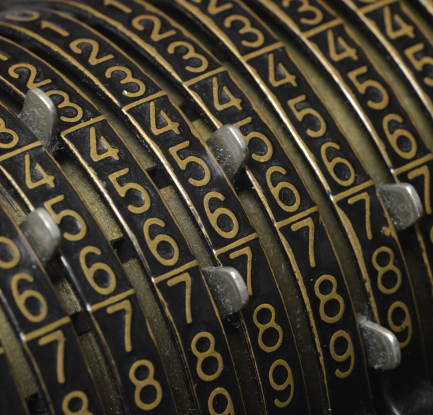
\includegraphics[width=11cm]{odhner_square_100dpi.jpg}
  \end{figure}

  {\Large --- Fast and Reproducible Data Processing ---}

  \vfill
  { Anders Berkeman, Carl Drougge, and Sofia H\"orberg}\\
  {\tiny{version: \inputfile{gitrevision}}}
\end{center}
\thispagestyle{empty}


\newpage
\thispagestyle{empty}
\section*{Document History}

\begin{tabular}{rrp{8cm}}
 date       & git hash          & description\\[0.75ex]
 2018-04-23 & \texttt{772990f4} & First open version.\\
 2018-05-28 & \texttt{a6d6750b} & Updated parts of Urd chapters.\\
 2019-06-11 & \texttt{24b4b6c2} & Major makeover.\\
 2019-06-24 & \texttt{db47cc19} & More on \texttt{depend\_extra}, valid column names, appeding columns in
  synthesis, and some formatting.\\
 2020-01-22 & \texttt{04fb2389} &  New class based interface.\\
 2020-02-14 & \texttt{562e8d10} & PyPI dev release.\\

 2020-04-22 & \texttt{54031595} & PyPI dev release.
 Relative paths in configfile, \texttt{link\_result()} in build
 scripts, \texttt{Job.files()}, s/daemon/server/g.\\

 2020-10-12 & \texttt{\inputfile{gitrevision}} & PyPI dev release,
 updated chapters 3 -- 8.  Missing in this version: \texttt{board} and
 latest class additions.\\
\end{tabular}


\newpage
\tableofcontents

\chapter{Introduction}
%%%%%%%%%%%%%%%%%%%%%%%%%%%%%%%%%%%%%%%%%%%%%%%%%%%%%%%%%%%%%%%%%%%%%%%%%%%%
%                                                                          %
% Copyright (c) 2018 eBay Inc.                                             %
%                                                                          %
% Licensed under the Apache License, Version 2.0 (the "License");          %
% you may not use this file except in compliance with the License.         %
% You may obtain a copy of the License at                                  %
%                                                                          %
%  http://www.apache.org/licenses/LICENSE-2.0                              %
%                                                                          %
% Unless required by applicable law or agreed to in writing, software      %
% distributed under the License is distributed on an "AS IS" BASIS,        %
% WITHOUT WARRANTIES OR CONDITIONS OF ANY KIND, either express or implied. %
% See the License for the specific language governing permissions and      %
% limitations under the License.                                           %
%                                                                          %
%%%%%%%%%%%%%%%%%%%%%%%%%%%%%%%%%%%%%%%%%%%%%%%%%%%%%%%%%%%%%%%%%%%%%%%%%%%%

The Accelerator is a tool for fast reproducible data processing,
capable of working at high speed with terabytes of data with billions
of rows on a single computer.  The speed in combination with its
unique capabilites to ensure reproducibility makes the Accelerator a
good choice for tasks where it is important to keep track of how data
and results are connected.  Typical applications include all kinds of
data analysis work as well as live production systems for tasks such
as recommender systems, and more.  The Accelerator has a small
footprint, few dependencies, and runs on laptops as well as rack
servers.

The Accelerator was first used in 2012, and has been continuously developed and
improved since.  It has been in use in projects for companies like
\textsl{Safeway}, \textsl{Starbucks}, \textsl{eBay}, \textsl{Ericsson},
and \textsl{Vodafone}.  Most project have been related to data
analysis, some to optimisation, and some projects have been
recommendation systems running live for years.  The Accelerator has
been the core of these projects.  In 2016, the Accelerator was
acquired by Ebay, who contributed it to the open source community
early 2018.

Data set sizes in these projects range from a few hundred lines up to
several tens of billions rows and many columns.  The number of
items in a dataset used in a live system was well above $10^{11}$, and
this was handled with ease on a \emph{single} 32 core computer.

The authors are Anders Berkeman, Carl Drougge, and Sofia H\"orberg.
More than 1600 commits have been removed to clean up the open version
of the code base, and about 1000 new commits have been created since
the Accelerator was open sourced.  Extensive testing has been done by
Stefan H{\aa}konsson.  The Accelerator is written in Python, with the
exception of some critical parts that are written in the C programming
language.



\section{Main Design Goals}
The Accelerator is designed to process log-files in ``CSV''-like
formats\footnote{CSV is short for Comma Separated Values, but any
separator character can be used.  CSV files store data into rows and
columns of text.  Classical ``databases'' could be generated from, and
dumped to, CSV-files.}.  Log files bring determinism (i.e.\
reproducibility) and transparency, and most data can be represented in
this format.  The Accelerator is developed bottom up for high
performance and simplicity, and the main design goals are:
\begin{itemize}

\item[] \textsl{Parallel processing} should be made simple.  Modern computers
  come with several cores, it should be straightforward to make use of
  them.

\item[] Data rates should be as fast as possible, i.e.\ close to the hardware
bounds.  It should be possible to process \textsl{large datasets},
  even on commodity hardware.

\item[] Any processing step should be \textsl{reproducible}.
The Accelerator maps any output result to its corresponding input data and
processing source code.

\item[] Never recompute old results, always ``recycle'' old jobs, when
  possible.  Also, \textsl{sharing results} between multiple users should be
  effortless.

\item[] \textsl{Organise} and keep track of all jobs, files, and results in
  order to work with projects having 100.000s of input files and lots
  of programs and scripts processing them.
  
\end{itemize}
In addition, the Accelerator is originally designed to be used at all
levels of a project, including data analysis, algorithm development,
as well as production.  Nevertheless, it still excels as a pure data
analysis or data processing tool.


\chapter{Overview}
%%%%%%%%%%%%%%%%%%%%%%%%%%%%%%%%%%%%%%%%%%%%%%%%%%%%%%%%%%%%%%%%%%%%%%%%%%%%
%                                                                          %
% Copyright (c) 2018 eBay Inc.                                             %
% Modifications copyright (c) 2019-2021 Anders Berkeman                    %
%                                                                          %
% Licensed under the Apache License, Version 2.0 (the "License");          %
% you may not use this file except in compliance with the License.         %
% You may obtain a copy of the License at                                  %
%                                                                          %
%  http://www.apache.org/licenses/LICENSE-2.0                              %
%                                                                          %
% Unless required by applicable law or agreed to in writing, software      %
% distributed under the License is distributed on an "AS IS" BASIS,        %
% WITHOUT WARRANTIES OR CONDITIONS OF ANY KIND, either express or implied. %
% See the License for the specific language governing permissions and      %
% limitations under the License.                                           %
%                                                                          %
%%%%%%%%%%%%%%%%%%%%%%%%%%%%%%%%%%%%%%%%%%%%%%%%%%%%%%%%%%%%%%%%%%%%%%%%%%%%


This chapter presents an overview of the Accelerator's features in a
rather non-formal way.  It is based on an article published on the
eBay Tech Blog website.



\section{High Level View}
The Accelerator is a client-server based application, and from a high
level, it can be visualised like in figure~\ref{fig:overview}.

\begin{figure}[h!]
  \begin{center}
    %%%%%%%%%%%%%%%%%%%%%%%%%%%%%%%%%%%%%%%%%%%%%%%%%%%%%%%%%%%%%%%%%%%%%%%%%%%%
%                                                                          %
% Copyright (c) 2018 eBay Inc.                                             %
% Modifications copyright (c) 2019-2021 Anders Berkeman                    %
%                                                                          %
% Licensed under the Apache License, Version 2.0 (the "License");          %
% you may not use this file except in compliance with the License.         %
% You may obtain a copy of the License at                                  %
%                                                                          %
%  http://www.apache.org/licenses/LICENSE-2.0                              %
%                                                                          %
% Unless required by applicable law or agreed to in writing, software      %
% distributed under the License is distributed on an "AS IS" BASIS,        %
% WITHOUT WARRANTIES OR CONDITIONS OF ANY KIND, either express or implied. %
% See the License for the specific language governing permissions and      %
% limitations under the License.                                           %
%                                                                          %
%%%%%%%%%%%%%%%%%%%%%%%%%%%%%%%%%%%%%%%%%%%%%%%%%%%%%%%%%%%%%%%%%%%%%%%%%%%%


This chapter presents an overview of the Accelerator's features in a
rather non-formal way.  It is based on an article published on the
eBay Tech Blog website.



\section{High Level View}
The Accelerator is a client-server based application, and from a high
level, it can be visualised like in figure~\ref{fig:overview}.

\begin{figure}[h!]
  \begin{center}
    %%%%%%%%%%%%%%%%%%%%%%%%%%%%%%%%%%%%%%%%%%%%%%%%%%%%%%%%%%%%%%%%%%%%%%%%%%%%
%                                                                          %
% Copyright (c) 2018 eBay Inc.                                             %
% Modifications copyright (c) 2019-2021 Anders Berkeman                    %
%                                                                          %
% Licensed under the Apache License, Version 2.0 (the "License");          %
% you may not use this file except in compliance with the License.         %
% You may obtain a copy of the License at                                  %
%                                                                          %
%  http://www.apache.org/licenses/LICENSE-2.0                              %
%                                                                          %
% Unless required by applicable law or agreed to in writing, software      %
% distributed under the License is distributed on an "AS IS" BASIS,        %
% WITHOUT WARRANTIES OR CONDITIONS OF ANY KIND, either express or implied. %
% See the License for the specific language governing permissions and      %
% limitations under the License.                                           %
%                                                                          %
%%%%%%%%%%%%%%%%%%%%%%%%%%%%%%%%%%%%%%%%%%%%%%%%%%%%%%%%%%%%%%%%%%%%%%%%%%%%


This chapter presents an overview of the Accelerator's features in a
rather non-formal way.  It is based on an article published on the
eBay Tech Blog website.



\section{High Level View}
The Accelerator is a client-server based application, and from a high
level, it can be visualised like in figure~\ref{fig:overview}.

\begin{figure}[h!]
  \begin{center}
    \input{figures/overview.pdftex_t}
    \caption{High level view of the Accelerator framework.  See text
      for details.}
    \label{fig:overview}
  \end{center}
\end{figure}

In the figure, the client side, with shell commands and web interface,
is on the left, and the server side, with job databases is to the
right.  The Accelerator executes \textsl{build scripts}, that issue
\textsl{jobs} on the server.  These jobs are stored in the server's
job databases for later retreival.  There are two databases, one for
storing everything related to a job's execution, called the
\textsl{workdir}, and one transaction log used for storing
meta-information about built jobs.  The workdir will contain all
inputs, source code, parameters, and outputs of all executed jobs,
whereas the job log database ensures reproducibility and transparency,
and it will be further discussed in chapter~\ref{chap:urd}.



\section{Jobs}
The basic operation of the Accelerator is to execute small Python
programs called \textsl{methods}.  A method is nothing but a Python
program with one or a few special functions that are used to execute
code sequentially or in parallel and to pass parameters and results.
A method that has completed execution is called a \textsl{job}.

Jobs are stored in \textsl{job directories}.  A dedicated directory in
the workdir will be created for each new job, and this directory will
contain all information regarding the job, such as its input
parameters, stored files, return values, profiling information, Python
interpreter version and path, and more.

The Accelerator has a database that keeps track of all jobs that has
been run.  This avoids unnecessary re-computing in favour of re-using
previously computed results.  Re-using jobs does not only speed up
processing and encourage incremental design, but also makes it
transparent which code and which data that was used for any particular
result, minimising these kind of uncertainties to zero.


\subsection{A Very Simple Job:  ``Hello, World''}
Here's an example of a very simple method.  It does not take any input
parameters and does almost nothing, it will just return the string
``\texttt{hello world}'' and exit.
\begin{python}
def synthesis():
    return "hello world"
\end{python}
Everything inside the \texttt{synthesis()}-function is run once
without any parallelisation.  In order to get this method to execute,
it is called from a \textsl{build script} looking something like this
\begin{python}
def main(urd)
    job = urd.build('hello_world')
    print(job.load())
\end{python}
The \texttt{urd} object made available by the \texttt{main()}-function
contains functions for job building and organisation, and is described
in chapter~\ref{chap:urd} and section~\ref{sec:classes:urd}.  This
build script is then run by a shell command like this
\begin{shell}
ax run
\end{shell}
The \texttt{build()}-call will instruct the server to execute the
\texttt{hello\_world} method.  During its execution, a job directory
will be created that contains everyting associated with the build
process.  When the \texttt{build()}-call is completed, a job object, of type
\texttt{Job}, is returned to the program.  This object provides a
convenient interface to the data in the corresponding job directory,
and contains member functions such as \texttt{.load()}, that is used
in the example to read back the returned value from the job.


\subsection{Jobs Can Only be Run Once}
If the build script is executed again, the \texttt{hello\_world} job
will not be re-built, simply because the Accelerator remembers that
the job has been built in the past, and its associated information is
stored in a job directory.  Instead, the Accelerator immediately
returns a job object representing the previous run.  This means that
from a user's perspective, there is no visible difference between
running a job for the first time or re-using results from an existing
run!  In order to have the method executing again, either the source
code or input parameters has to change.  If there are changes, the
method will be re-executed, and a new job will be created that
reflects these changes.


\subsection{Back to the ``Hello, World'' Example}
Figure~\ref{fig:execflow-hello-world} illustrates the dispatch of the
\texttt{hello\_world} method.  The created job gets the \textsl{jobid}
\texttt{test-0}, and parts of the corresponding job directory
information is shown in green.  (Jobids are job identifiers, that are
named by their corresponding \textsl{workdir} plus an integer counter
value.)  The job directory contains several files, of which the most
important are
\begin{itemize}
\item[] \texttt{setup.json}, containing job meta information;
\item[] \texttt{result.pickle}, containing the returned data; and
\item[] \texttt{method.tar.gz}, containing the method's source code.
\end{itemize}

\begin{figure}[b]
  \begin{center}
    \input{figures/job0.pdftex_t}
    \caption{A simple hello world program, represented as graph and
      work directory.}
    \label{fig:execflow-hello-world}
  \end{center}
\end{figure}

The \texttt{Job} object provides a convenient way to access files and
data stored in this directory.  For example, as we've already seen,
the job's return value can be loaded into a variable using the
\texttt{.load()} function.



\subsection{Workdirs and Sharing Jobs}

Workdirs are used to store jobs.  There can be more than one workdir,
and different workdirs can be used separate jobs into different
physical locations.  The Accelerator can be set up to have any number
of workdirs associated, but only one is used for writing.

If the same workdir is entered into two or more different user's
configuration files, the workdir and its contents will be shared
between the users.  Each Accelerator server will update its knowledge
about the contents of all workdirs before executing a build script, to
make sure that the latest jobs are taken into account.  In addition,
the job log database, as described in chapter~\ref{chap:urd}, is
designed for efficient re-use and sharing of particularly interesting
jobs.


\subsection{Linking Jobs}

Using jobs, complex tasks can be split into several smaller
operations.  Jobs can be connected so that the next job will depend on
the result of a previous job or set of jobs, and so on.

To continue the simple hello world example, assume for a second that
the \texttt{hello\_world}-job is computationally expensive, and that
it returns a result that is to be used as input to further processing.
To keep things simple, this further processing is represented by
printing the result to standard output.  A new method
\texttt{print\_result} is created, and it goes like this
\begin{python}
jobs = ('hello_world_job',)

def synthesis():
    data = jobs.hello_world_job.load() 
    print(data)
\end{python}
This method expects the \texttt{hello\_world\_job} input parameter to
be provided at execution time, and it is accomplished by the following
extended build script
\begin{python}
def main(urd):
    job1 = urd.build('hello_world')
    job2 = urd.build('print_result', hello_world_job=job1)
\end{python}
The \texttt{print\_result} method then loads the result from the
provided job and prints its contents to \texttt{stdout}.  Note that
this method does not return anything.

Figure~\ref{fig:execflow-print-result} illustrates the situation.
(Note the direction of the arrow: the second job, \texttt{test-1} has
\texttt{test-0} as input parameter, but \texttt{test-0} does not know
of any jobs run in the future.  Hence, arrows point to previous jobs.)

\begin{figure}[b]
  \begin{center}
    \input{figures/job0job1.pdftex_t}
    \caption{Job \texttt{test-0}, is used as input to the
      \texttt{print\_result} job.}
    \label{fig:execflow-print-result}
  \end{center}
\end{figure}

The example shows how a complex task may be split into several jobs,
each reading intermediate results from previous jobs.  The Accelerator
will keep track of all job dependencies, so there is no doubt which
jobs that are run when and on which data.  Furthermore, since the
Accelerator remembers if a job has been executed before, it will link
and re-use previous jobs when possible.  This may bring a significant
improvement in execution speed.  Furthermore, a re-used job is a proof
of that the code, input- and output data is unchanged and connected.


\section{Datasets: Storing Data}

The \texttt{dataset} is the Accelerator's default storage type for
small or large quantities of data, designed for parallel processing
and high performance.  Datasets are built on top of jobs, so
\emph{datasets are created by methods and stored in job directories,
  just like any job result.}

Internally, data in a dataset is stored in a row-column format, and is
typically \emph{sliced} into a fixed number of slices to allow
efficient parallel access, see figure~\ref{fig:dataset}. Columns are
accessed independently, so there is no overhead in reading a single or
a set of columns.  Only the data relevant for a task is read from
disk.


\begin{figure}[h!]
  \begin{center}
    \input{figures/dataset_files.pdftex_t}
    \caption{A dataset containing three columns, $A$, $B$, and $C$
      stored using two slices.  Each dotted box corresponds to a file,
      so there are two files for each column, allowing for parallel
      read of the data using two processes.}
    \label{fig:dataset}
  \end{center}
\end{figure}

Furthermore, datasets may be \textsl{hash partitioned}, so that
slice-membership is based on the hash value of a given column.
Partitioning base on, for example, a column containing some ID string
will puy all rows corresponding to any particular ID in a single slice
only.  In many practical applications, hash partitioning makes
parallel processes independent, minimising the need for complicated
merging operations.  This is explained further in
section~\ref{sec:slicing_and_hashing}.



\subsection{Importing Data}

A project typically starts with \textsl{importing} some data from a
file on disk.  The bundled method \texttt{csvimport} is designed to
parse a plethora of ``comma separated values''-file formats and store
the data as a dataset.  See figure~\ref{fig:dataset_csvimport}.
\begin{figure}[b]
  \begin{center}
    \input{figures/import_file1.pdftex_t}
    \caption{Importing \texttt{file0.txt}.}
    \label{fig:dataset_csvimport}
  \end{center}
\end{figure}
The method takes several input options in addition to the mandatory
filename to control the import process.  Here is an example
invocation
\begin{python}
def main(urd):
    jid = urd.build('csvimport', filename='file0.txt')
\end{python}
When executed, the created dataset will be stored in the resulting job
directory, and the name of the dataset will by default be the jobid
plus the string \texttt{default}.  For example, if the
\texttt{csvimport} jobid is \texttt{imp-0}, the dataset will be
referenced by \texttt{imp-0/default}.  In this case, and always when
there is no ambiguity, the jobid alone (\texttt{imp-0}) could be used
too, for simplicity.  In general, a job could contain any number of
datasets, but a single dataset is a common case.




\subsection{Linking Datasets, Chaining}

Just like jobs can be linked to each other, datasets can link to each
other too.  Since datasets are build on top of jobs, this is
straightforward.  Assume the file \texttt{file0.txt} is imported into
dataset \texttt{imp-0/default}, and that there is more data like it
stored in the file \texttt{file1.txt}.  The second file is imported
with a link to the first dataset, see
figure~\ref{fig:dataset_csvimport_chain}.
\begin{figure}[t]
  \begin{center}
    \input{figures/import_file0file1.pdftex_t}
    \caption{Chaining the import of \texttt{file1.txt} to the previous
      import of \texttt{file0.txt}.}
    \label{fig:dataset_csvimport_chain}
  \end{center}
\end{figure}
The \texttt{imp-1} (or \texttt{imp-1/default}) dataset reference can
now be used to access all data imported from \textsl{both} files!

Linking datasets containing related content is called \emph{chaining},
and this is particularly convenient when dealing with data that grows
over time.  A good example is any kind of \emph{log} data, such as
logs of transactions, user interactions, and similar.  Using chaining,
datasets can be with more rows just by linking, which is a lightweight
constant time operation.



\subsection{Adding New Columns to a Dataset}
In the previous section it was shown that datasets can be chained and
thereby grow in number of rows.  A dataset chain is created simply by
linking one dataset to the other, so the overhead is minimal.  In this
section it is shown that by the same principles, it is equally simple
to add new columns to existing datasets.  Adding columns is a common
operation and the Accelerator handles this situation efficiently using
links.

The idea is very simple.  Assume a ``source'' dataset to which one or
more new columns should be added.  A new dataset is created containing
\textsl{only} the new column(s), and while creating it, the
constructor is instructed to link all the source dataset's columns to
the new dataset such that the new dataset appears to contain all
columns from both datasets.  (Note that this linking is similar to but
different from chaining.)

Accessing the new dataset will transparently access all the columns in
both the new and the source dataset in parallel, making it
indistinguishable from a single dataset.  See
Figure~\ref{fig:dep_dataset_append_column}.

\begin{figure}[b]
  \begin{center}
    \input{figures/dataset_append_column.pdftex_t}
    \caption{Adding one new column to the source dataset.}
    \label{fig:dep_dataset_append_column}
  \end{center}
\end{figure}

A common case is to compute new columns based on existing ones.  In
this case, values are written to the new columns in the new dataset
while reading from the iterator iterating over the existing columns in
the source dataset.  This will be discussed in detail in
section~\ref{sec:appending_new_columns}



\subsection{Multiple Datasets in a Job}

Typically, a method creates a single dataset in the job directory, but
there is no limit to how many datasets that could be created and
stored in a single job directory.  This leads to some interesting
applications.

One application for keeping multiple datasets in a job is when data is
split into subsets based on some condition.  This could, for example,
be when a dataset is split into a training set and a test set.  One
way to achieve this using the Accelerator is by creating a Boolean
column that tells if the current row is train or test data, followed
by a job that splits the dataset in two based on the value on that
column.  See Figure~\ref{fig:dep_dataset_csvimport_chain}.

\begin{figure}[h!]
  \hspace{1cm}
  \input{figures/filter_dataset.pdftex_t}
  \caption{\texttt{job-1} separates the dataset
    \texttt{job-0/default} into two new datasets, named
    \texttt{job-1/train} and \texttt{job-1/test}.}
  \label{fig:dep_dataset_csvimport_chain}
\end{figure}

In the setup of figure~\ref{fig:dep_dataset_csvimport_chain} we have
full tracking from either \texttt{train} or \texttt{test} datasets.
If we want to know the source of one of these sets, we just follow the
links back to the previous jobs until we reach the source job.  In the
figure, \texttt{job-0} may for example be a \texttt{csvimport} job,
and will therefore contain the name of the input file in its
parameters.  Thus, it is straightforward to link any data to its
source.

Splitting a dataset into parts creates ``physical'' isolation while
still keeping all the data at the same place.  No data is lost in the
process, and this is good for transparency reasons.  For example, a
following method may iterate over \textsl{both} datasets in
\texttt{job-1} and by that read the complete dataset.



\subsection{Parallel Dataset Access and Hash Partitioning}
As shown earlier in this chapter, data in datasets is stored in
multiple files for two reasons.  The first reason is that we can read
only the columns that we need, without overhead, and the second reason
is that it allows fast parallel reads.  The parameter \texttt{slices}
determines how many slices that the dataset should be partitioned
into, and it also sets the number of parallel process that is used for
processing the dataset.  There is always one process for each slice of
the dataset, and each process operates on a unique part of the
dataset.

Datasets can be partitioned, or sliced, in different ways.  One
obvious way is to use round robin, where each consecutive data row is
written to the next slice, modulo the number of slices.  This leads to
``well balanced'' datasets with approximately equal number of rows per
slice.  Another alternative to slicing is to slice based on the hash
value of a particular column's values.  Using this method, all rows
with the same value in the hash column end up in the same slice.  This
is efficient for many parallel processing tasks, and will be described
in detail later on.




\subsection{Dataset Column Types}

There are large a number of useful types available for dataset
columns.  They include \textsl{floating} and \textsl{integer point
  numbers}, \textsl{Booleans}, \textsl{timestamps}, several
\textsl{string types} (handling all kinds of string encodings), and
\textsl{json} as well as \textsl{pickle} types for storing arbitrary
data collections.  Most of these types come with advanced parsers,
making importing data from text files straightforward with
deterministic handling of errors, overflows, and so on.



\subsection{Dataset Attributes}
The dataset has a number of attributes associated with it, such as
shape, number of rows, column names and types, and more.
An attribute is accessed like this
\begin{python}
datasets = ('source',)
def synthesis():
    print(datasets.source.shape)
    print(datasets.source.columns)
\end{python}
and so on.


%%%%%%%%%%%%%%%%%%%%%%%%%%%%%%%%%%%%%%%%%%%%%%%%%%%%%%%%%%%%%%%%%%%%%%%%%%%%%%%%

\section{Iterators: Working with Data}

Data in a dataset is typically accessed using an \emph{iterator} that
reads and streams one dataset slice at a time to a CPU core.  The
parallel processing capabilities of the Accelerator makes it possible
to dispatch a set of parallel iterators, one for each slice, in order
to have efficient parallel processing of the whole dataset.

This section shows how iterators are used for reading data, how to
take advantage of slicing to have parallel processing, and how to
efficiently create new datasets.


\subsection{Iterator Basics}

Basic iterator functionality is introduced here using an example.
Assume a dataset that has a column containing movie titles named
\texttt{movie}, and the problem is to extract the ten most frequently
occuring movies.  Here's a complete method solving this problem
\begin{python}
from collections import Counter
datasets = ('source',)

def synthesis():
    c = Counter(datasets.source.iterate(None, 'movie'))
    top10 = c.most_common(10)
    print(top10)
    return top10
\end{python}
This will print the ten most common movie titles and their
corresponding counts in the \texttt{source} dataset.  The code will
run on a single CPU core, because we use the single-process
\texttt{synthesis()} function, which is called and executed only once.
The \texttt{dataset.iterate()} (class-)method therefore has to read
through all slices, one at a time, in a serial fashion, and this is
reflected by the first argument to the iterator being \pyNone.  The
method also returns the variable \texttt{top10} so that it can be used
by other methods.



\subsection{Parallel Execution}
It is easy to write parallel programs using the Accelerator.  The fact
that data in a dataset is sliced into disjoint sets and files makes
parallel processing of data straightforward.  Here's a slightly
modified version of the program from the previous section that will
now execute in parallel
\begin{python}
def analysis(sliceno):
    return Counter(datasets.source.iterate(sliceno, 'movie'))

def synthesis(analysis_res)
    c = analysis_res.merge_auto()
    top10 = c.most_common(10)
    return top10
\end{python}
For larger datasets, this parallel version of the movie title counter
will run much faster.  Here, \texttt{.iterate()} is moved inside the
\texttt{analysis()} function.  This function is forked once for each
slice, and the argument \texttt{sliceno} will contain an integer
between zero and the number of slices minus one.  The returned value
from the analysis functions will be available as input to the
synthesis function in the \texttt{analysis\_res} Python iterable.  It
is possible to merge the results explicitly, but the this iterable
comes with a rather magic method \texttt{merge\_auto()}, that merges
the results from all slices into one based on the data type.  It can
for example merge \texttt{Counter}s, \texttt{set}s, and composed types
like \texttt{set}s of \texttt{Counter}s, and so on.


\subsection{Iterating over Several Columns}
Since each column is stored independently in a dataset, there is no
overhead from reading a subset of a dataset's columns.  In the
previous section we've seen how to iterate over a single column using
\texttt{.iterate()}.  Iterating over more columns is straightforward
by feeding a list of column names to \texttt{.iterate()}, like in this
example
\begin{python}
from collections import defaultdict
datasets = ('source',)

def analysis(sliceno):
    user2movieset = defaultdict(set)
    for user, movie in datasets.source.iterate(sliceno, ('user', 'movie')):
        user2movieset[user].add(movie)
    return user2movieset
\end{python}
This example creates a lookup dictionary from users to sets of movies.
Note that in this case, we would like to have the dataset hashed on
the \texttt{user} column, so that each user appears in exactly one slice.
This will make later merging (if necessary) much easier.

It is also possible to iterate over all columns by specifying an empty
list of columns or by using the value \pyNone.
\begin{python}
...
def analysis(sliceno):
    for columns in datasets.source.iterate(sliceno, None):
        ...
\end{python}
Here, \texttt{columns} will be a list of values, one for each column
in the dataset, in sorted column name order.


\subsection{Iterating over Dataset Chains}

The \texttt{iterate} function is used to iterate over a single
dataset.  There is a corresponding function, \texttt{iterate\_chain},
that is used for iterating over chains of datasets.  This function
takes a number of arguments, such as
\begin{itemize}
\item[] \texttt{length}, i.e.\ the number of datasets to iterate over.
  By default, it will iterate over all datasets in the chain.
\item[] \texttt{callbacks}, functions that can be called before and/or
  after each dataset in a chain.  Very useful for aggregating data
  between datasets.
\item[] \texttt{stop\_id} which stops iterating at a certain dataset.
  This dataset could be from \textsl{another} job's parameters, so we
  can for example iterate exactly over all new datasets not covered by
  a previous job.
\item[] \texttt{range}, which allows for iterating over a range of
  data.
\end{itemize}
The \texttt{range} options is based on the max/min values stored for
each column in the dataset.  Assuming that the chain is sorted, one
can for example set
\begin{python}
range={timestamp, ('2016-01-01', '2016-01-31')}
\end{python}
in order to get rows within the specified range only.  Using
\texttt{range=} is quite costly, since it requires each row in the
dataset chain with dates within the range to be checked against the
range criterion.  Therefore, there is a \texttt{sloppy} version that
iterates over complete datasets in the chain that contains at least
one row with a date within the range.  This runs at full speed, and is
useful, for example, to very quickly produce histograms or plots of
subsets of a huge dataset.



\subsection{Job Execution Flow and Result Passing}

Execution of code in a method is either parallel or serial depending
on which function is used to encapsulate it.  There are three
functions in a method that are called from the Accelerator when a
method is running, and they are \texttt{prepare()},
\texttt{analysis()}, and \texttt{synthesis()}.  All three may exist in
the same method, and at least one is required.  When the method
executes, they are called one after the other.
\begin{itemize}
\item[] \texttt{prepare()} is executed first.  The returned value is
  available in the variable \texttt{prepare\_res}.
\item[] \texttt{analysis()} is run in parallel processes, one for each
  slice.  It is called after completion of, and actually forked from
  \texttt{prepare()}.  Common input parameters are \texttt{sliceno},
  holding the number of the current process instance, and
  \texttt{prepare\_res}.  The return value for each process becomes
  available in the \texttt{analysis\_res} variable.
\item[] \texttt{synthesis()} is called after the last
  \texttt{analysis()}-process is completed.  It is typically used to
  aggregate parallel results created by \texttt{analysis()} and takes
  both \texttt{prepare\_res} and \texttt{analysis\_res} as optional
  parameters.  The latter is an iterator of the results from the
  parallel processes.
\end{itemize}
Figure~\ref{fig:prepanasyn} shows the execution order from top to
bottom, and the data passed between functions in coloured branches.
\texttt{prepare()} is executed first, and its return value is
available to both the \texttt{analysis()} and \texttt{synthesis()}
functions.  There are \texttt{slices} (a configurable parameter)
number of parallel \texttt{analysis()} processes, and their output is
available to the \texttt{synthesis()} function, which is executed
last.

Return values from any of the three functions may be stored in the
job's directory making them available to other jobs.


\begin{figure}[t]
  \begin{center}
    \input{figures/prepanasyn.pdftex_t}
    \caption{Execution flow and result propagation in a method.}
    \label{fig:prepanasyn}
  \end{center}
\end{figure}



\subsection{Job Parameters}
\label{sec:jobparams}
We've seen how completed jobs can be used as input to new
jobs.  Jobs are one of three kinds of input parameters that
a job can take.  Here the input parameters are summarised:
\begin{itemize}
\item[] \texttt{jobs}, a set, or list, of identifiers to previously executed jobs;
\item[] \texttt{options}, a dictionary of options; and
\item[] \texttt{datasets}, a set, or list, of input \textsl{datasets}.
\end{itemize}
See Figure~\ref{fig:execflow}.  Parameters are entered as global
variables early in the method's source.


\begin{figure}[b]
  \begin{center}
    \input{figures/execflow.pdftex_t}
    \caption{Execution flow of a method.  The method takes optionally
      three kinds of parameters: \texttt{options}, \texttt{jobs},
      and \texttt{datasets}.}
    \label{fig:execflow}
  \end{center}
\end{figure}





\section{A Class Based Programming Model}
The Accelerator is based on an class based paradigm.  Access the the
Accelerator's build in functions and parameters are typically done
through a few \textsl{objects} that are populated by the running
Accelerator.

    \caption{High level view of the Accelerator framework.  See text
      for details.}
    \label{fig:overview}
  \end{center}
\end{figure}

In the figure, the client side, with shell commands and web interface,
is on the left, and the server side, with job databases is to the
right.  The Accelerator executes \textsl{build scripts}, that issue
\textsl{jobs} on the server.  These jobs are stored in the server's
job databases for later retreival.  There are two databases, one for
storing everything related to a job's execution, called the
\textsl{workdir}, and one transaction log used for storing
meta-information about built jobs.  The workdir will contain all
inputs, source code, parameters, and outputs of all executed jobs,
whereas the job log database ensures reproducibility and transparency,
and it will be further discussed in chapter~\ref{chap:urd}.



\section{Jobs}
The basic operation of the Accelerator is to execute small Python
programs called \textsl{methods}.  A method is nothing but a Python
program with one or a few special functions that are used to execute
code sequentially or in parallel and to pass parameters and results.
A method that has completed execution is called a \textsl{job}.

Jobs are stored in \textsl{job directories}.  A dedicated directory in
the workdir will be created for each new job, and this directory will
contain all information regarding the job, such as its input
parameters, stored files, return values, profiling information, Python
interpreter version and path, and more.

The Accelerator has a database that keeps track of all jobs that has
been run.  This avoids unnecessary re-computing in favour of re-using
previously computed results.  Re-using jobs does not only speed up
processing and encourage incremental design, but also makes it
transparent which code and which data that was used for any particular
result, minimising these kind of uncertainties to zero.


\subsection{A Very Simple Job:  ``Hello, World''}
Here's an example of a very simple method.  It does not take any input
parameters and does almost nothing, it will just return the string
``\texttt{hello world}'' and exit.
\begin{python}
def synthesis():
    return "hello world"
\end{python}
Everything inside the \texttt{synthesis()}-function is run once
without any parallelisation.  In order to get this method to execute,
it is called from a \textsl{build script} looking something like this
\begin{python}
def main(urd)
    job = urd.build('hello_world')
    print(job.load())
\end{python}
The \texttt{urd} object made available by the \texttt{main()}-function
contains functions for job building and organisation, and is described
in chapter~\ref{chap:urd} and section~\ref{sec:classes:urd}.  This
build script is then run by a shell command like this
\begin{shell}
ax run
\end{shell}
The \texttt{build()}-call will instruct the server to execute the
\texttt{hello\_world} method.  During its execution, a job directory
will be created that contains everyting associated with the build
process.  When the \texttt{build()}-call is completed, a job object, of type
\texttt{Job}, is returned to the program.  This object provides a
convenient interface to the data in the corresponding job directory,
and contains member functions such as \texttt{.load()}, that is used
in the example to read back the returned value from the job.


\subsection{Jobs Can Only be Run Once}
If the build script is executed again, the \texttt{hello\_world} job
will not be re-built, simply because the Accelerator remembers that
the job has been built in the past, and its associated information is
stored in a job directory.  Instead, the Accelerator immediately
returns a job object representing the previous run.  This means that
from a user's perspective, there is no visible difference between
running a job for the first time or re-using results from an existing
run!  In order to have the method executing again, either the source
code or input parameters has to change.  If there are changes, the
method will be re-executed, and a new job will be created that
reflects these changes.


\subsection{Back to the ``Hello, World'' Example}
Figure~\ref{fig:execflow-hello-world} illustrates the dispatch of the
\texttt{hello\_world} method.  The created job gets the \textsl{jobid}
\texttt{test-0}, and parts of the corresponding job directory
information is shown in green.  (Jobids are job identifiers, that are
named by their corresponding \textsl{workdir} plus an integer counter
value.)  The job directory contains several files, of which the most
important are
\begin{itemize}
\item[] \texttt{setup.json}, containing job meta information;
\item[] \texttt{result.pickle}, containing the returned data; and
\item[] \texttt{method.tar.gz}, containing the method's source code.
\end{itemize}

\begin{figure}[b]
  \begin{center}
    \input{figures/job0.pdftex_t}
    \caption{A simple hello world program, represented as graph and
      work directory.}
    \label{fig:execflow-hello-world}
  \end{center}
\end{figure}

The \texttt{Job} object provides a convenient way to access files and
data stored in this directory.  For example, as we've already seen,
the job's return value can be loaded into a variable using the
\texttt{.load()} function.



\subsection{Workdirs and Sharing Jobs}

Workdirs are used to store jobs.  There can be more than one workdir,
and different workdirs can be used separate jobs into different
physical locations.  The Accelerator can be set up to have any number
of workdirs associated, but only one is used for writing.

If the same workdir is entered into two or more different user's
configuration files, the workdir and its contents will be shared
between the users.  Each Accelerator server will update its knowledge
about the contents of all workdirs before executing a build script, to
make sure that the latest jobs are taken into account.  In addition,
the job log database, as described in chapter~\ref{chap:urd}, is
designed for efficient re-use and sharing of particularly interesting
jobs.


\subsection{Linking Jobs}

Using jobs, complex tasks can be split into several smaller
operations.  Jobs can be connected so that the next job will depend on
the result of a previous job or set of jobs, and so on.

To continue the simple hello world example, assume for a second that
the \texttt{hello\_world}-job is computationally expensive, and that
it returns a result that is to be used as input to further processing.
To keep things simple, this further processing is represented by
printing the result to standard output.  A new method
\texttt{print\_result} is created, and it goes like this
\begin{python}
jobs = ('hello_world_job',)

def synthesis():
    data = jobs.hello_world_job.load() 
    print(data)
\end{python}
This method expects the \texttt{hello\_world\_job} input parameter to
be provided at execution time, and it is accomplished by the following
extended build script
\begin{python}
def main(urd):
    job1 = urd.build('hello_world')
    job2 = urd.build('print_result', hello_world_job=job1)
\end{python}
The \texttt{print\_result} method then loads the result from the
provided job and prints its contents to \texttt{stdout}.  Note that
this method does not return anything.

Figure~\ref{fig:execflow-print-result} illustrates the situation.
(Note the direction of the arrow: the second job, \texttt{test-1} has
\texttt{test-0} as input parameter, but \texttt{test-0} does not know
of any jobs run in the future.  Hence, arrows point to previous jobs.)

\begin{figure}[b]
  \begin{center}
    \input{figures/job0job1.pdftex_t}
    \caption{Job \texttt{test-0}, is used as input to the
      \texttt{print\_result} job.}
    \label{fig:execflow-print-result}
  \end{center}
\end{figure}

The example shows how a complex task may be split into several jobs,
each reading intermediate results from previous jobs.  The Accelerator
will keep track of all job dependencies, so there is no doubt which
jobs that are run when and on which data.  Furthermore, since the
Accelerator remembers if a job has been executed before, it will link
and re-use previous jobs when possible.  This may bring a significant
improvement in execution speed.  Furthermore, a re-used job is a proof
of that the code, input- and output data is unchanged and connected.


\section{Datasets: Storing Data}

The \texttt{dataset} is the Accelerator's default storage type for
small or large quantities of data, designed for parallel processing
and high performance.  Datasets are built on top of jobs, so
\emph{datasets are created by methods and stored in job directories,
  just like any job result.}

Internally, data in a dataset is stored in a row-column format, and is
typically \emph{sliced} into a fixed number of slices to allow
efficient parallel access, see figure~\ref{fig:dataset}. Columns are
accessed independently, so there is no overhead in reading a single or
a set of columns.  Only the data relevant for a task is read from
disk.


\begin{figure}[h!]
  \begin{center}
    \input{figures/dataset_files.pdftex_t}
    \caption{A dataset containing three columns, $A$, $B$, and $C$
      stored using two slices.  Each dotted box corresponds to a file,
      so there are two files for each column, allowing for parallel
      read of the data using two processes.}
    \label{fig:dataset}
  \end{center}
\end{figure}

Furthermore, datasets may be \textsl{hash partitioned}, so that
slice-membership is based on the hash value of a given column.
Partitioning base on, for example, a column containing some ID string
will puy all rows corresponding to any particular ID in a single slice
only.  In many practical applications, hash partitioning makes
parallel processes independent, minimising the need for complicated
merging operations.  This is explained further in
section~\ref{sec:slicing_and_hashing}.



\subsection{Importing Data}

A project typically starts with \textsl{importing} some data from a
file on disk.  The bundled method \texttt{csvimport} is designed to
parse a plethora of ``comma separated values''-file formats and store
the data as a dataset.  See figure~\ref{fig:dataset_csvimport}.
\begin{figure}[b]
  \begin{center}
    \input{figures/import_file1.pdftex_t}
    \caption{Importing \texttt{file0.txt}.}
    \label{fig:dataset_csvimport}
  \end{center}
\end{figure}
The method takes several input options in addition to the mandatory
filename to control the import process.  Here is an example
invocation
\begin{python}
def main(urd):
    jid = urd.build('csvimport', filename='file0.txt')
\end{python}
When executed, the created dataset will be stored in the resulting job
directory, and the name of the dataset will by default be the jobid
plus the string \texttt{default}.  For example, if the
\texttt{csvimport} jobid is \texttt{imp-0}, the dataset will be
referenced by \texttt{imp-0/default}.  In this case, and always when
there is no ambiguity, the jobid alone (\texttt{imp-0}) could be used
too, for simplicity.  In general, a job could contain any number of
datasets, but a single dataset is a common case.




\subsection{Linking Datasets, Chaining}

Just like jobs can be linked to each other, datasets can link to each
other too.  Since datasets are build on top of jobs, this is
straightforward.  Assume the file \texttt{file0.txt} is imported into
dataset \texttt{imp-0/default}, and that there is more data like it
stored in the file \texttt{file1.txt}.  The second file is imported
with a link to the first dataset, see
figure~\ref{fig:dataset_csvimport_chain}.
\begin{figure}[t]
  \begin{center}
    \input{figures/import_file0file1.pdftex_t}
    \caption{Chaining the import of \texttt{file1.txt} to the previous
      import of \texttt{file0.txt}.}
    \label{fig:dataset_csvimport_chain}
  \end{center}
\end{figure}
The \texttt{imp-1} (or \texttt{imp-1/default}) dataset reference can
now be used to access all data imported from \textsl{both} files!

Linking datasets containing related content is called \emph{chaining},
and this is particularly convenient when dealing with data that grows
over time.  A good example is any kind of \emph{log} data, such as
logs of transactions, user interactions, and similar.  Using chaining,
datasets can be with more rows just by linking, which is a lightweight
constant time operation.



\subsection{Adding New Columns to a Dataset}
In the previous section it was shown that datasets can be chained and
thereby grow in number of rows.  A dataset chain is created simply by
linking one dataset to the other, so the overhead is minimal.  In this
section it is shown that by the same principles, it is equally simple
to add new columns to existing datasets.  Adding columns is a common
operation and the Accelerator handles this situation efficiently using
links.

The idea is very simple.  Assume a ``source'' dataset to which one or
more new columns should be added.  A new dataset is created containing
\textsl{only} the new column(s), and while creating it, the
constructor is instructed to link all the source dataset's columns to
the new dataset such that the new dataset appears to contain all
columns from both datasets.  (Note that this linking is similar to but
different from chaining.)

Accessing the new dataset will transparently access all the columns in
both the new and the source dataset in parallel, making it
indistinguishable from a single dataset.  See
Figure~\ref{fig:dep_dataset_append_column}.

\begin{figure}[b]
  \begin{center}
    \input{figures/dataset_append_column.pdftex_t}
    \caption{Adding one new column to the source dataset.}
    \label{fig:dep_dataset_append_column}
  \end{center}
\end{figure}

A common case is to compute new columns based on existing ones.  In
this case, values are written to the new columns in the new dataset
while reading from the iterator iterating over the existing columns in
the source dataset.  This will be discussed in detail in
section~\ref{sec:appending_new_columns}



\subsection{Multiple Datasets in a Job}

Typically, a method creates a single dataset in the job directory, but
there is no limit to how many datasets that could be created and
stored in a single job directory.  This leads to some interesting
applications.

One application for keeping multiple datasets in a job is when data is
split into subsets based on some condition.  This could, for example,
be when a dataset is split into a training set and a test set.  One
way to achieve this using the Accelerator is by creating a Boolean
column that tells if the current row is train or test data, followed
by a job that splits the dataset in two based on the value on that
column.  See Figure~\ref{fig:dep_dataset_csvimport_chain}.

\begin{figure}[h!]
  \hspace{1cm}
  \input{figures/filter_dataset.pdftex_t}
  \caption{\texttt{job-1} separates the dataset
    \texttt{job-0/default} into two new datasets, named
    \texttt{job-1/train} and \texttt{job-1/test}.}
  \label{fig:dep_dataset_csvimport_chain}
\end{figure}

In the setup of figure~\ref{fig:dep_dataset_csvimport_chain} we have
full tracking from either \texttt{train} or \texttt{test} datasets.
If we want to know the source of one of these sets, we just follow the
links back to the previous jobs until we reach the source job.  In the
figure, \texttt{job-0} may for example be a \texttt{csvimport} job,
and will therefore contain the name of the input file in its
parameters.  Thus, it is straightforward to link any data to its
source.

Splitting a dataset into parts creates ``physical'' isolation while
still keeping all the data at the same place.  No data is lost in the
process, and this is good for transparency reasons.  For example, a
following method may iterate over \textsl{both} datasets in
\texttt{job-1} and by that read the complete dataset.



\subsection{Parallel Dataset Access and Hash Partitioning}
As shown earlier in this chapter, data in datasets is stored in
multiple files for two reasons.  The first reason is that we can read
only the columns that we need, without overhead, and the second reason
is that it allows fast parallel reads.  The parameter \texttt{slices}
determines how many slices that the dataset should be partitioned
into, and it also sets the number of parallel process that is used for
processing the dataset.  There is always one process for each slice of
the dataset, and each process operates on a unique part of the
dataset.

Datasets can be partitioned, or sliced, in different ways.  One
obvious way is to use round robin, where each consecutive data row is
written to the next slice, modulo the number of slices.  This leads to
``well balanced'' datasets with approximately equal number of rows per
slice.  Another alternative to slicing is to slice based on the hash
value of a particular column's values.  Using this method, all rows
with the same value in the hash column end up in the same slice.  This
is efficient for many parallel processing tasks, and will be described
in detail later on.




\subsection{Dataset Column Types}

There are large a number of useful types available for dataset
columns.  They include \textsl{floating} and \textsl{integer point
  numbers}, \textsl{Booleans}, \textsl{timestamps}, several
\textsl{string types} (handling all kinds of string encodings), and
\textsl{json} as well as \textsl{pickle} types for storing arbitrary
data collections.  Most of these types come with advanced parsers,
making importing data from text files straightforward with
deterministic handling of errors, overflows, and so on.



\subsection{Dataset Attributes}
The dataset has a number of attributes associated with it, such as
shape, number of rows, column names and types, and more.
An attribute is accessed like this
\begin{python}
datasets = ('source',)
def synthesis():
    print(datasets.source.shape)
    print(datasets.source.columns)
\end{python}
and so on.


%%%%%%%%%%%%%%%%%%%%%%%%%%%%%%%%%%%%%%%%%%%%%%%%%%%%%%%%%%%%%%%%%%%%%%%%%%%%%%%%

\section{Iterators: Working with Data}

Data in a dataset is typically accessed using an \emph{iterator} that
reads and streams one dataset slice at a time to a CPU core.  The
parallel processing capabilities of the Accelerator makes it possible
to dispatch a set of parallel iterators, one for each slice, in order
to have efficient parallel processing of the whole dataset.

This section shows how iterators are used for reading data, how to
take advantage of slicing to have parallel processing, and how to
efficiently create new datasets.


\subsection{Iterator Basics}

Basic iterator functionality is introduced here using an example.
Assume a dataset that has a column containing movie titles named
\texttt{movie}, and the problem is to extract the ten most frequently
occuring movies.  Here's a complete method solving this problem
\begin{python}
from collections import Counter
datasets = ('source',)

def synthesis():
    c = Counter(datasets.source.iterate(None, 'movie'))
    top10 = c.most_common(10)
    print(top10)
    return top10
\end{python}
This will print the ten most common movie titles and their
corresponding counts in the \texttt{source} dataset.  The code will
run on a single CPU core, because we use the single-process
\texttt{synthesis()} function, which is called and executed only once.
The \texttt{dataset.iterate()} (class-)method therefore has to read
through all slices, one at a time, in a serial fashion, and this is
reflected by the first argument to the iterator being \pyNone.  The
method also returns the variable \texttt{top10} so that it can be used
by other methods.



\subsection{Parallel Execution}
It is easy to write parallel programs using the Accelerator.  The fact
that data in a dataset is sliced into disjoint sets and files makes
parallel processing of data straightforward.  Here's a slightly
modified version of the program from the previous section that will
now execute in parallel
\begin{python}
def analysis(sliceno):
    return Counter(datasets.source.iterate(sliceno, 'movie'))

def synthesis(analysis_res)
    c = analysis_res.merge_auto()
    top10 = c.most_common(10)
    return top10
\end{python}
For larger datasets, this parallel version of the movie title counter
will run much faster.  Here, \texttt{.iterate()} is moved inside the
\texttt{analysis()} function.  This function is forked once for each
slice, and the argument \texttt{sliceno} will contain an integer
between zero and the number of slices minus one.  The returned value
from the analysis functions will be available as input to the
synthesis function in the \texttt{analysis\_res} Python iterable.  It
is possible to merge the results explicitly, but the this iterable
comes with a rather magic method \texttt{merge\_auto()}, that merges
the results from all slices into one based on the data type.  It can
for example merge \texttt{Counter}s, \texttt{set}s, and composed types
like \texttt{set}s of \texttt{Counter}s, and so on.


\subsection{Iterating over Several Columns}
Since each column is stored independently in a dataset, there is no
overhead from reading a subset of a dataset's columns.  In the
previous section we've seen how to iterate over a single column using
\texttt{.iterate()}.  Iterating over more columns is straightforward
by feeding a list of column names to \texttt{.iterate()}, like in this
example
\begin{python}
from collections import defaultdict
datasets = ('source',)

def analysis(sliceno):
    user2movieset = defaultdict(set)
    for user, movie in datasets.source.iterate(sliceno, ('user', 'movie')):
        user2movieset[user].add(movie)
    return user2movieset
\end{python}
This example creates a lookup dictionary from users to sets of movies.
Note that in this case, we would like to have the dataset hashed on
the \texttt{user} column, so that each user appears in exactly one slice.
This will make later merging (if necessary) much easier.

It is also possible to iterate over all columns by specifying an empty
list of columns or by using the value \pyNone.
\begin{python}
...
def analysis(sliceno):
    for columns in datasets.source.iterate(sliceno, None):
        ...
\end{python}
Here, \texttt{columns} will be a list of values, one for each column
in the dataset, in sorted column name order.


\subsection{Iterating over Dataset Chains}

The \texttt{iterate} function is used to iterate over a single
dataset.  There is a corresponding function, \texttt{iterate\_chain},
that is used for iterating over chains of datasets.  This function
takes a number of arguments, such as
\begin{itemize}
\item[] \texttt{length}, i.e.\ the number of datasets to iterate over.
  By default, it will iterate over all datasets in the chain.
\item[] \texttt{callbacks}, functions that can be called before and/or
  after each dataset in a chain.  Very useful for aggregating data
  between datasets.
\item[] \texttt{stop\_id} which stops iterating at a certain dataset.
  This dataset could be from \textsl{another} job's parameters, so we
  can for example iterate exactly over all new datasets not covered by
  a previous job.
\item[] \texttt{range}, which allows for iterating over a range of
  data.
\end{itemize}
The \texttt{range} options is based on the max/min values stored for
each column in the dataset.  Assuming that the chain is sorted, one
can for example set
\begin{python}
range={timestamp, ('2016-01-01', '2016-01-31')}
\end{python}
in order to get rows within the specified range only.  Using
\texttt{range=} is quite costly, since it requires each row in the
dataset chain with dates within the range to be checked against the
range criterion.  Therefore, there is a \texttt{sloppy} version that
iterates over complete datasets in the chain that contains at least
one row with a date within the range.  This runs at full speed, and is
useful, for example, to very quickly produce histograms or plots of
subsets of a huge dataset.



\subsection{Job Execution Flow and Result Passing}

Execution of code in a method is either parallel or serial depending
on which function is used to encapsulate it.  There are three
functions in a method that are called from the Accelerator when a
method is running, and they are \texttt{prepare()},
\texttt{analysis()}, and \texttt{synthesis()}.  All three may exist in
the same method, and at least one is required.  When the method
executes, they are called one after the other.
\begin{itemize}
\item[] \texttt{prepare()} is executed first.  The returned value is
  available in the variable \texttt{prepare\_res}.
\item[] \texttt{analysis()} is run in parallel processes, one for each
  slice.  It is called after completion of, and actually forked from
  \texttt{prepare()}.  Common input parameters are \texttt{sliceno},
  holding the number of the current process instance, and
  \texttt{prepare\_res}.  The return value for each process becomes
  available in the \texttt{analysis\_res} variable.
\item[] \texttt{synthesis()} is called after the last
  \texttt{analysis()}-process is completed.  It is typically used to
  aggregate parallel results created by \texttt{analysis()} and takes
  both \texttt{prepare\_res} and \texttt{analysis\_res} as optional
  parameters.  The latter is an iterator of the results from the
  parallel processes.
\end{itemize}
Figure~\ref{fig:prepanasyn} shows the execution order from top to
bottom, and the data passed between functions in coloured branches.
\texttt{prepare()} is executed first, and its return value is
available to both the \texttt{analysis()} and \texttt{synthesis()}
functions.  There are \texttt{slices} (a configurable parameter)
number of parallel \texttt{analysis()} processes, and their output is
available to the \texttt{synthesis()} function, which is executed
last.

Return values from any of the three functions may be stored in the
job's directory making them available to other jobs.


\begin{figure}[t]
  \begin{center}
    \input{figures/prepanasyn.pdftex_t}
    \caption{Execution flow and result propagation in a method.}
    \label{fig:prepanasyn}
  \end{center}
\end{figure}



\subsection{Job Parameters}
\label{sec:jobparams}
We've seen how completed jobs can be used as input to new
jobs.  Jobs are one of three kinds of input parameters that
a job can take.  Here the input parameters are summarised:
\begin{itemize}
\item[] \texttt{jobs}, a set, or list, of identifiers to previously executed jobs;
\item[] \texttt{options}, a dictionary of options; and
\item[] \texttt{datasets}, a set, or list, of input \textsl{datasets}.
\end{itemize}
See Figure~\ref{fig:execflow}.  Parameters are entered as global
variables early in the method's source.


\begin{figure}[b]
  \begin{center}
    \input{figures/execflow.pdftex_t}
    \caption{Execution flow of a method.  The method takes optionally
      three kinds of parameters: \texttt{options}, \texttt{jobs},
      and \texttt{datasets}.}
    \label{fig:execflow}
  \end{center}
\end{figure}





\section{A Class Based Programming Model}
The Accelerator is based on an class based paradigm.  Access the the
Accelerator's build in functions and parameters are typically done
through a few \textsl{objects} that are populated by the running
Accelerator.

    \caption{High level view of the Accelerator framework.  See text
      for details.}
    \label{fig:overview}
  \end{center}
\end{figure}

In the figure, the client side, with shell commands and web interface,
is on the left, and the server side, with job databases is to the
right.  The Accelerator executes \textsl{build scripts}, that issue
\textsl{jobs} on the server.  These jobs are stored in the server's
job databases for later retreival.  There are two databases, one for
storing everything related to a job's execution, called the
\textsl{workdir}, and one transaction log used for storing
meta-information about built jobs.  The workdir will contain all
inputs, source code, parameters, and outputs of all executed jobs,
whereas the job log database ensures reproducibility and transparency,
and it will be further discussed in chapter~\ref{chap:urd}.



\section{Jobs}
The basic operation of the Accelerator is to execute small Python
programs called \textsl{methods}.  A method is nothing but a Python
program with one or a few special functions that are used to execute
code sequentially or in parallel and to pass parameters and results.
A method that has completed execution is called a \textsl{job}.

Jobs are stored in \textsl{job directories}.  A dedicated directory in
the workdir will be created for each new job, and this directory will
contain all information regarding the job, such as its input
parameters, stored files, return values, profiling information, Python
interpreter version and path, and more.

The Accelerator has a database that keeps track of all jobs that has
been run.  This avoids unnecessary re-computing in favour of re-using
previously computed results.  Re-using jobs does not only speed up
processing and encourage incremental design, but also makes it
transparent which code and which data that was used for any particular
result, minimising these kind of uncertainties to zero.


\subsection{A Very Simple Job:  ``Hello, World''}
Here's an example of a very simple method.  It does not take any input
parameters and does almost nothing, it will just return the string
``\texttt{hello world}'' and exit.
\begin{python}
def synthesis():
    return "hello world"
\end{python}
Everything inside the \texttt{synthesis()}-function is run once
without any parallelisation.  In order to get this method to execute,
it is called from a \textsl{build script} looking something like this
\begin{python}
def main(urd)
    job = urd.build('hello_world')
    print(job.load())
\end{python}
The \texttt{urd} object made available by the \texttt{main()}-function
contains functions for job building and organisation, and is described
in chapter~\ref{chap:urd} and section~\ref{sec:classes:urd}.  This
build script is then run by a shell command like this
\begin{shell}
ax run
\end{shell}
The \texttt{build()}-call will instruct the server to execute the
\texttt{hello\_world} method.  During its execution, a job directory
will be created that contains everyting associated with the build
process.  When the \texttt{build()}-call is completed, a job object, of type
\texttt{Job}, is returned to the program.  This object provides a
convenient interface to the data in the corresponding job directory,
and contains member functions such as \texttt{.load()}, that is used
in the example to read back the returned value from the job.


\subsection{Jobs Can Only be Run Once}
If the build script is executed again, the \texttt{hello\_world} job
will not be re-built, simply because the Accelerator remembers that
the job has been built in the past, and its associated information is
stored in a job directory.  Instead, the Accelerator immediately
returns a job object representing the previous run.  This means that
from a user's perspective, there is no visible difference between
running a job for the first time or re-using results from an existing
run!  In order to have the method executing again, either the source
code or input parameters has to change.  If there are changes, the
method will be re-executed, and a new job will be created that
reflects these changes.


\subsection{Back to the ``Hello, World'' Example}
Figure~\ref{fig:execflow-hello-world} illustrates the dispatch of the
\texttt{hello\_world} method.  The created job gets the \textsl{jobid}
\texttt{test-0}, and parts of the corresponding job directory
information is shown in green.  (Jobids are job identifiers, that are
named by their corresponding \textsl{workdir} plus an integer counter
value.)  The job directory contains several files, of which the most
important are
\begin{itemize}
\item[] \texttt{setup.json}, containing job meta information;
\item[] \texttt{result.pickle}, containing the returned data; and
\item[] \texttt{method.tar.gz}, containing the method's source code.
\end{itemize}

\begin{figure}[b]
  \begin{center}
    \input{figures/job0.pdftex_t}
    \caption{A simple hello world program, represented as graph and
      work directory.}
    \label{fig:execflow-hello-world}
  \end{center}
\end{figure}

The \texttt{Job} object provides a convenient way to access files and
data stored in this directory.  For example, as we've already seen,
the job's return value can be loaded into a variable using the
\texttt{.load()} function.



\subsection{Workdirs and Sharing Jobs}

Workdirs are used to store jobs.  There can be more than one workdir,
and different workdirs can be used separate jobs into different
physical locations.  The Accelerator can be set up to have any number
of workdirs associated, but only one is used for writing.

If the same workdir is entered into two or more different user's
configuration files, the workdir and its contents will be shared
between the users.  Each Accelerator server will update its knowledge
about the contents of all workdirs before executing a build script, to
make sure that the latest jobs are taken into account.  In addition,
the job log database, as described in chapter~\ref{chap:urd}, is
designed for efficient re-use and sharing of particularly interesting
jobs.


\subsection{Linking Jobs}

Using jobs, complex tasks can be split into several smaller
operations.  Jobs can be connected so that the next job will depend on
the result of a previous job or set of jobs, and so on.

To continue the simple hello world example, assume for a second that
the \texttt{hello\_world}-job is computationally expensive, and that
it returns a result that is to be used as input to further processing.
To keep things simple, this further processing is represented by
printing the result to standard output.  A new method
\texttt{print\_result} is created, and it goes like this
\begin{python}
jobs = ('hello_world_job',)

def synthesis():
    data = jobs.hello_world_job.load() 
    print(data)
\end{python}
This method expects the \texttt{hello\_world\_job} input parameter to
be provided at execution time, and it is accomplished by the following
extended build script
\begin{python}
def main(urd):
    job1 = urd.build('hello_world')
    job2 = urd.build('print_result', hello_world_job=job1)
\end{python}
The \texttt{print\_result} method then loads the result from the
provided job and prints its contents to \texttt{stdout}.  Note that
this method does not return anything.

Figure~\ref{fig:execflow-print-result} illustrates the situation.
(Note the direction of the arrow: the second job, \texttt{test-1} has
\texttt{test-0} as input parameter, but \texttt{test-0} does not know
of any jobs run in the future.  Hence, arrows point to previous jobs.)

\begin{figure}[b]
  \begin{center}
    \input{figures/job0job1.pdftex_t}
    \caption{Job \texttt{test-0}, is used as input to the
      \texttt{print\_result} job.}
    \label{fig:execflow-print-result}
  \end{center}
\end{figure}

The example shows how a complex task may be split into several jobs,
each reading intermediate results from previous jobs.  The Accelerator
will keep track of all job dependencies, so there is no doubt which
jobs that are run when and on which data.  Furthermore, since the
Accelerator remembers if a job has been executed before, it will link
and re-use previous jobs when possible.  This may bring a significant
improvement in execution speed.  Furthermore, a re-used job is a proof
of that the code, input- and output data is unchanged and connected.


\section{Datasets: Storing Data}

The \texttt{dataset} is the Accelerator's default storage type for
small or large quantities of data, designed for parallel processing
and high performance.  Datasets are built on top of jobs, so
\emph{datasets are created by methods and stored in job directories,
  just like any job result.}

Internally, data in a dataset is stored in a row-column format, and is
typically \emph{sliced} into a fixed number of slices to allow
efficient parallel access, see figure~\ref{fig:dataset}. Columns are
accessed independently, so there is no overhead in reading a single or
a set of columns.  Only the data relevant for a task is read from
disk.


\begin{figure}[h!]
  \begin{center}
    \input{figures/dataset_files.pdftex_t}
    \caption{A dataset containing three columns, $A$, $B$, and $C$
      stored using two slices.  Each dotted box corresponds to a file,
      so there are two files for each column, allowing for parallel
      read of the data using two processes.}
    \label{fig:dataset}
  \end{center}
\end{figure}

Furthermore, datasets may be \textsl{hash partitioned}, so that
slice-membership is based on the hash value of a given column.
Partitioning base on, for example, a column containing some ID string
will puy all rows corresponding to any particular ID in a single slice
only.  In many practical applications, hash partitioning makes
parallel processes independent, minimising the need for complicated
merging operations.  This is explained further in
section~\ref{sec:slicing_and_hashing}.



\subsection{Importing Data}

A project typically starts with \textsl{importing} some data from a
file on disk.  The bundled method \texttt{csvimport} is designed to
parse a plethora of ``comma separated values''-file formats and store
the data as a dataset.  See figure~\ref{fig:dataset_csvimport}.
\begin{figure}[b]
  \begin{center}
    \input{figures/import_file1.pdftex_t}
    \caption{Importing \texttt{file0.txt}.}
    \label{fig:dataset_csvimport}
  \end{center}
\end{figure}
The method takes several input options in addition to the mandatory
filename to control the import process.  Here is an example
invocation
\begin{python}
def main(urd):
    jid = urd.build('csvimport', filename='file0.txt')
\end{python}
When executed, the created dataset will be stored in the resulting job
directory, and the name of the dataset will by default be the jobid
plus the string \texttt{default}.  For example, if the
\texttt{csvimport} jobid is \texttt{imp-0}, the dataset will be
referenced by \texttt{imp-0/default}.  In this case, and always when
there is no ambiguity, the jobid alone (\texttt{imp-0}) could be used
too, for simplicity.  In general, a job could contain any number of
datasets, but a single dataset is a common case.




\subsection{Linking Datasets, Chaining}

Just like jobs can be linked to each other, datasets can link to each
other too.  Since datasets are build on top of jobs, this is
straightforward.  Assume the file \texttt{file0.txt} is imported into
dataset \texttt{imp-0/default}, and that there is more data like it
stored in the file \texttt{file1.txt}.  The second file is imported
with a link to the first dataset, see
figure~\ref{fig:dataset_csvimport_chain}.
\begin{figure}[t]
  \begin{center}
    \input{figures/import_file0file1.pdftex_t}
    \caption{Chaining the import of \texttt{file1.txt} to the previous
      import of \texttt{file0.txt}.}
    \label{fig:dataset_csvimport_chain}
  \end{center}
\end{figure}
The \texttt{imp-1} (or \texttt{imp-1/default}) dataset reference can
now be used to access all data imported from \textsl{both} files!

Linking datasets containing related content is called \emph{chaining},
and this is particularly convenient when dealing with data that grows
over time.  A good example is any kind of \emph{log} data, such as
logs of transactions, user interactions, and similar.  Using chaining,
datasets can be with more rows just by linking, which is a lightweight
constant time operation.



\subsection{Adding New Columns to a Dataset}
In the previous section it was shown that datasets can be chained and
thereby grow in number of rows.  A dataset chain is created simply by
linking one dataset to the other, so the overhead is minimal.  In this
section it is shown that by the same principles, it is equally simple
to add new columns to existing datasets.  Adding columns is a common
operation and the Accelerator handles this situation efficiently using
links.

The idea is very simple.  Assume a ``source'' dataset to which one or
more new columns should be added.  A new dataset is created containing
\textsl{only} the new column(s), and while creating it, the
constructor is instructed to link all the source dataset's columns to
the new dataset such that the new dataset appears to contain all
columns from both datasets.  (Note that this linking is similar to but
different from chaining.)

Accessing the new dataset will transparently access all the columns in
both the new and the source dataset in parallel, making it
indistinguishable from a single dataset.  See
Figure~\ref{fig:dep_dataset_append_column}.

\begin{figure}[b]
  \begin{center}
    \input{figures/dataset_append_column.pdftex_t}
    \caption{Adding one new column to the source dataset.}
    \label{fig:dep_dataset_append_column}
  \end{center}
\end{figure}

A common case is to compute new columns based on existing ones.  In
this case, values are written to the new columns in the new dataset
while reading from the iterator iterating over the existing columns in
the source dataset.  This will be discussed in detail in
section~\ref{sec:appending_new_columns}



\subsection{Multiple Datasets in a Job}

Typically, a method creates a single dataset in the job directory, but
there is no limit to how many datasets that could be created and
stored in a single job directory.  This leads to some interesting
applications.

One application for keeping multiple datasets in a job is when data is
split into subsets based on some condition.  This could, for example,
be when a dataset is split into a training set and a test set.  One
way to achieve this using the Accelerator is by creating a Boolean
column that tells if the current row is train or test data, followed
by a job that splits the dataset in two based on the value on that
column.  See Figure~\ref{fig:dep_dataset_csvimport_chain}.

\begin{figure}[h!]
  \hspace{1cm}
  \input{figures/filter_dataset.pdftex_t}
  \caption{\texttt{job-1} separates the dataset
    \texttt{job-0/default} into two new datasets, named
    \texttt{job-1/train} and \texttt{job-1/test}.}
  \label{fig:dep_dataset_csvimport_chain}
\end{figure}

In the setup of figure~\ref{fig:dep_dataset_csvimport_chain} we have
full tracking from either \texttt{train} or \texttt{test} datasets.
If we want to know the source of one of these sets, we just follow the
links back to the previous jobs until we reach the source job.  In the
figure, \texttt{job-0} may for example be a \texttt{csvimport} job,
and will therefore contain the name of the input file in its
parameters.  Thus, it is straightforward to link any data to its
source.

Splitting a dataset into parts creates ``physical'' isolation while
still keeping all the data at the same place.  No data is lost in the
process, and this is good for transparency reasons.  For example, a
following method may iterate over \textsl{both} datasets in
\texttt{job-1} and by that read the complete dataset.



\subsection{Parallel Dataset Access and Hash Partitioning}
As shown earlier in this chapter, data in datasets is stored in
multiple files for two reasons.  The first reason is that we can read
only the columns that we need, without overhead, and the second reason
is that it allows fast parallel reads.  The parameter \texttt{slices}
determines how many slices that the dataset should be partitioned
into, and it also sets the number of parallel process that is used for
processing the dataset.  There is always one process for each slice of
the dataset, and each process operates on a unique part of the
dataset.

Datasets can be partitioned, or sliced, in different ways.  One
obvious way is to use round robin, where each consecutive data row is
written to the next slice, modulo the number of slices.  This leads to
``well balanced'' datasets with approximately equal number of rows per
slice.  Another alternative to slicing is to slice based on the hash
value of a particular column's values.  Using this method, all rows
with the same value in the hash column end up in the same slice.  This
is efficient for many parallel processing tasks, and will be described
in detail later on.




\subsection{Dataset Column Types}

There are large a number of useful types available for dataset
columns.  They include \textsl{floating} and \textsl{integer point
  numbers}, \textsl{Booleans}, \textsl{timestamps}, several
\textsl{string types} (handling all kinds of string encodings), and
\textsl{json} as well as \textsl{pickle} types for storing arbitrary
data collections.  Most of these types come with advanced parsers,
making importing data from text files straightforward with
deterministic handling of errors, overflows, and so on.



\subsection{Dataset Attributes}
The dataset has a number of attributes associated with it, such as
shape, number of rows, column names and types, and more.
An attribute is accessed like this
\begin{python}
datasets = ('source',)
def synthesis():
    print(datasets.source.shape)
    print(datasets.source.columns)
\end{python}
and so on.


%%%%%%%%%%%%%%%%%%%%%%%%%%%%%%%%%%%%%%%%%%%%%%%%%%%%%%%%%%%%%%%%%%%%%%%%%%%%%%%%

\section{Iterators: Working with Data}

Data in a dataset is typically accessed using an \emph{iterator} that
reads and streams one dataset slice at a time to a CPU core.  The
parallel processing capabilities of the Accelerator makes it possible
to dispatch a set of parallel iterators, one for each slice, in order
to have efficient parallel processing of the whole dataset.

This section shows how iterators are used for reading data, how to
take advantage of slicing to have parallel processing, and how to
efficiently create new datasets.


\subsection{Iterator Basics}

Basic iterator functionality is introduced here using an example.
Assume a dataset that has a column containing movie titles named
\texttt{movie}, and the problem is to extract the ten most frequently
occuring movies.  Here's a complete method solving this problem
\begin{python}
from collections import Counter
datasets = ('source',)

def synthesis():
    c = Counter(datasets.source.iterate(None, 'movie'))
    top10 = c.most_common(10)
    print(top10)
    return top10
\end{python}
This will print the ten most common movie titles and their
corresponding counts in the \texttt{source} dataset.  The code will
run on a single CPU core, because we use the single-process
\texttt{synthesis()} function, which is called and executed only once.
The \texttt{dataset.iterate()} (class-)method therefore has to read
through all slices, one at a time, in a serial fashion, and this is
reflected by the first argument to the iterator being \pyNone.  The
method also returns the variable \texttt{top10} so that it can be used
by other methods.



\subsection{Parallel Execution}
It is easy to write parallel programs using the Accelerator.  The fact
that data in a dataset is sliced into disjoint sets and files makes
parallel processing of data straightforward.  Here's a slightly
modified version of the program from the previous section that will
now execute in parallel
\begin{python}
def analysis(sliceno):
    return Counter(datasets.source.iterate(sliceno, 'movie'))

def synthesis(analysis_res)
    c = analysis_res.merge_auto()
    top10 = c.most_common(10)
    return top10
\end{python}
For larger datasets, this parallel version of the movie title counter
will run much faster.  Here, \texttt{.iterate()} is moved inside the
\texttt{analysis()} function.  This function is forked once for each
slice, and the argument \texttt{sliceno} will contain an integer
between zero and the number of slices minus one.  The returned value
from the analysis functions will be available as input to the
synthesis function in the \texttt{analysis\_res} Python iterable.  It
is possible to merge the results explicitly, but the this iterable
comes with a rather magic method \texttt{merge\_auto()}, that merges
the results from all slices into one based on the data type.  It can
for example merge \texttt{Counter}s, \texttt{set}s, and composed types
like \texttt{set}s of \texttt{Counter}s, and so on.


\subsection{Iterating over Several Columns}
Since each column is stored independently in a dataset, there is no
overhead from reading a subset of a dataset's columns.  In the
previous section we've seen how to iterate over a single column using
\texttt{.iterate()}.  Iterating over more columns is straightforward
by feeding a list of column names to \texttt{.iterate()}, like in this
example
\begin{python}
from collections import defaultdict
datasets = ('source',)

def analysis(sliceno):
    user2movieset = defaultdict(set)
    for user, movie in datasets.source.iterate(sliceno, ('user', 'movie')):
        user2movieset[user].add(movie)
    return user2movieset
\end{python}
This example creates a lookup dictionary from users to sets of movies.
Note that in this case, we would like to have the dataset hashed on
the \texttt{user} column, so that each user appears in exactly one slice.
This will make later merging (if necessary) much easier.

It is also possible to iterate over all columns by specifying an empty
list of columns or by using the value \pyNone.
\begin{python}
...
def analysis(sliceno):
    for columns in datasets.source.iterate(sliceno, None):
        ...
\end{python}
Here, \texttt{columns} will be a list of values, one for each column
in the dataset, in sorted column name order.


\subsection{Iterating over Dataset Chains}

The \texttt{iterate} function is used to iterate over a single
dataset.  There is a corresponding function, \texttt{iterate\_chain},
that is used for iterating over chains of datasets.  This function
takes a number of arguments, such as
\begin{itemize}
\item[] \texttt{length}, i.e.\ the number of datasets to iterate over.
  By default, it will iterate over all datasets in the chain.
\item[] \texttt{callbacks}, functions that can be called before and/or
  after each dataset in a chain.  Very useful for aggregating data
  between datasets.
\item[] \texttt{stop\_id} which stops iterating at a certain dataset.
  This dataset could be from \textsl{another} job's parameters, so we
  can for example iterate exactly over all new datasets not covered by
  a previous job.
\item[] \texttt{range}, which allows for iterating over a range of
  data.
\end{itemize}
The \texttt{range} options is based on the max/min values stored for
each column in the dataset.  Assuming that the chain is sorted, one
can for example set
\begin{python}
range={timestamp, ('2016-01-01', '2016-01-31')}
\end{python}
in order to get rows within the specified range only.  Using
\texttt{range=} is quite costly, since it requires each row in the
dataset chain with dates within the range to be checked against the
range criterion.  Therefore, there is a \texttt{sloppy} version that
iterates over complete datasets in the chain that contains at least
one row with a date within the range.  This runs at full speed, and is
useful, for example, to very quickly produce histograms or plots of
subsets of a huge dataset.



\subsection{Job Execution Flow and Result Passing}

Execution of code in a method is either parallel or serial depending
on which function is used to encapsulate it.  There are three
functions in a method that are called from the Accelerator when a
method is running, and they are \texttt{prepare()},
\texttt{analysis()}, and \texttt{synthesis()}.  All three may exist in
the same method, and at least one is required.  When the method
executes, they are called one after the other.
\begin{itemize}
\item[] \texttt{prepare()} is executed first.  The returned value is
  available in the variable \texttt{prepare\_res}.
\item[] \texttt{analysis()} is run in parallel processes, one for each
  slice.  It is called after completion of, and actually forked from
  \texttt{prepare()}.  Common input parameters are \texttt{sliceno},
  holding the number of the current process instance, and
  \texttt{prepare\_res}.  The return value for each process becomes
  available in the \texttt{analysis\_res} variable.
\item[] \texttt{synthesis()} is called after the last
  \texttt{analysis()}-process is completed.  It is typically used to
  aggregate parallel results created by \texttt{analysis()} and takes
  both \texttt{prepare\_res} and \texttt{analysis\_res} as optional
  parameters.  The latter is an iterator of the results from the
  parallel processes.
\end{itemize}
Figure~\ref{fig:prepanasyn} shows the execution order from top to
bottom, and the data passed between functions in coloured branches.
\texttt{prepare()} is executed first, and its return value is
available to both the \texttt{analysis()} and \texttt{synthesis()}
functions.  There are \texttt{slices} (a configurable parameter)
number of parallel \texttt{analysis()} processes, and their output is
available to the \texttt{synthesis()} function, which is executed
last.

Return values from any of the three functions may be stored in the
job's directory making them available to other jobs.


\begin{figure}[t]
  \begin{center}
    \input{figures/prepanasyn.pdftex_t}
    \caption{Execution flow and result propagation in a method.}
    \label{fig:prepanasyn}
  \end{center}
\end{figure}



\subsection{Job Parameters}
\label{sec:jobparams}
We've seen how completed jobs can be used as input to new
jobs.  Jobs are one of three kinds of input parameters that
a job can take.  Here the input parameters are summarised:
\begin{itemize}
\item[] \texttt{jobs}, a set, or list, of identifiers to previously executed jobs;
\item[] \texttt{options}, a dictionary of options; and
\item[] \texttt{datasets}, a set, or list, of input \textsl{datasets}.
\end{itemize}
See Figure~\ref{fig:execflow}.  Parameters are entered as global
variables early in the method's source.


\begin{figure}[b]
  \begin{center}
    \input{figures/execflow.pdftex_t}
    \caption{Execution flow of a method.  The method takes optionally
      three kinds of parameters: \texttt{options}, \texttt{jobs},
      and \texttt{datasets}.}
    \label{fig:execflow}
  \end{center}
\end{figure}





\section{A Class Based Programming Model}
The Accelerator is based on an class based paradigm.  Access the the
Accelerator's build in functions and parameters are typically done
through a few \textsl{objects} that are populated by the running
Accelerator.


\chapter{Basic Build Scripting}
\label{chap:urd_basic}

Build scripts are used to instruct the Accelerator about which jobs to
build.  This chapter describes the basics of job building.  More
advanced features, using the \texttt{urd} server, is presented in
chapter~\ref{chap:urd}.


\section{Build Scripts}
Build scripts are executed by the \texttt{runner} server.  A build
script must contain the function \texttt{main} as shown below, because
this function is called by the runner.
\begin{python}
def main(urd):
    ...
\end{python}
At run time, the \texttt{runner} inserts an object of the \texttt{Urd}
class as argument to the \texttt{main} function.  This object has a
number of member functions and attributes useful for job building.  It
also records all jobs that are built, together with their input
parameters and some more meta information, that will be described in
the next sections.  This chapter will only cover the basic
possibilities provided by Urd.  A more comprehensive view will be
provided in the next chapter.

\subsection{Building a Job}
The \texttt{build} function is typically used to build a job from a
method.  Here is an example of how to build the method
\texttt{method1}:
\begin{python}
def main(urd):
    urd.build('method1')
\end{python}
The full syntax for the \texttt{build} function is as follows
\begin{python}
jobid = urd.build(method, options={}, datasets={}, jobids={}, name='', caption='')
\end{python}
All paramters are optional, and
the \texttt{options}, \texttt{datasets}, and \texttt{jobids}
parameters depend on the method to be executed.  The \texttt{name}
will override the default name, which is equal to the name of the
method, when the job is recorded by Urd.  This is useful if several
jobs are build based on the same method.  Naming them uniquely makes
it easier to tell them apart later.  In addition, it is also possible
to assign a caption to a job.

When the job is successfully built, the \texttt{build} function will
return a reference, a \textsl{jobid} to the job.  Similarly, if the
job already existed in an available \textsl{workspace}, the
\texttt{build} function will immediately return a jobid to that job
without executing anything.


In addition, a name and a caption may be specified too
\begin{python}
jobid = urd.build('method1', name='myjob', caption='looking for something')
\end{python}
The name will override the default name (which is the name of the
method) in the Urd list.  In this case, this job will now be referred
to as \texttt{myjob} (instead of default \texttt{method1}).  A jobid
to the finished job is returned upon successful completion.



\subsection{Handling Consecutive Jobs}
Using the output jobid from the \texttt{build} function, it is
straightforward to connect jobs in series.  For example
\begin{python}
jid_filter = urd.build('filter_data', datasets=dict(source=<some_input>))
jid_reduce = urd.build('reduce', datasets=dict(source=jid_filter))
\end{python}
In the example above, the first job, \texttt{filter\_data} creates a
new dataset from its input.  This is then forwarded to the second job,
\texttt{reduce}, using the jobid reference \texttt{jid\_filter}.

If the first method or its input data is changed, the job will run
again.  This will cause the jobid \texttt{jid\_filter} to change too,
which in turn will trig execution of the \texttt{reduce} job.



\subsection{Building Chained Jobs}
It is also possible to build chained jobs implicitly using the
\texttt{build\_chained} function
\begin{python}
jobid = urd.build_chained('method1', name='myjob')
\end{python}
which takes the same options as the standard \texttt{build} method,
with the exception that name is mandatory.  The method to be chained
must have a ``\texttt{previous}'' key in its \texttt{datasets}
parameter.  The latest job with the same name is looked up by the
runner, and the corresponding jobid is assigned to the
method's \texttt{datasets.previous}.



\subsection{Replaying Build Scripts}
Executing an unmodified build script again will not cause any new jobs
to be executed.  Instead, the Accelerator will fill in the jobids of
the existing jobs so that processing can continue immediately.  A
successful ``replay'' of a build script ensures the integrity and
dependencies of the calculations.  If nothing has changed, the same
result remains.  If, however, some of the code has been modified, the
Accelerator will compute new jobs, the result may be different, and
the user is notified.




\section{The Joblist Type}
It has already been metioned that Urd keeps track of all built jobs.
This information is stored in the \texttt{urd.joblist} variable.  This
variable is of type \texttt{JobList}, which is basically
a \texttt{list} with some additional features.  The \texttt{joblist}
is an ordered list of jobs and it can be pretty-printed like this
\begin{python}
def main(urd):
    jid1 = urd.build('first')
    jid2 = urd.build('second', jobids=dict(first=jid1))
    print(urd.joblist.pretty)
\end{python}
which results in
\begin{shell}
JobList(
   [  0]  first : TEST-38
   [  1] second : TEST-39
)
\end{shell}
Any job in the list can be accessed by its name, so for example the
jobid to the \texttt{first} job could be retrieved by
\begin{python}
urd.joblist['first'].jobid
\end{python}
Using the joblist, we can modify our example to
\begin{python}
def main(urd):
    urd.build('first')
    urd.build('second', jobids=dict(first=urd.joblist['first'].jobid))
\end{python}
The ``\texttt{.jobid}'' is a bit clumsy, but currently required to get
the actual jobid for the job.  It is required because each item in
the \texttt{joblist} has a \texttt{.jobid} and a \texttt{.method}.
Note that if there are several jobs created by the same method, they
will have the same key in the joblist.  This situation could be
resolved using unique names to the \texttt{name=} option to
the \texttt{build()}-function as mentioned earlier.

An important special case is that the \textsl{latest} jobid is always
accessible using \texttt{urd.joblist.jobid}, so the code example could
also be written
\begin{python}
def main(urd):
    urd.build('first')
    urd.build('second', jobids=dict(first=urd.joblist.jobid))
\end{python}

It is also possible to look up jobs by name in the \texttt{joblist}.
This is done using the \texttt{find} function
\begin{python}
urd.joblist.find('csvimport')
\end{python}
If there is more than one job matching, the last one will be returned.

Finally, it may be worth noting that the \texttt{Joblist} is actually
a \texttt{list}, so it is possible to access individual items like
this
\begin{python}
jl[3]
\end{python}
and slicing works, too
\begin{python}
jl[-2:]
\end{python}


\section{Configuration Information from the Daemon}
The dictionary \texttt{urd.info} contains configuration information
from the Accelerator daemon.  In particular, it contains these fields
\starttabletwo
\RPtwo \texttt{slices} & Configured number of slices.\\[1ex]
\RPtwo \texttt{urd} & An URL to the Urd server, if configured,
  \pyNone otherwise.\\[1ex]
\RPtwo \texttt{result\_directory} & see section~\ref{}.\\[1ex]
\RPtwo \texttt{common\_directory} & see section~\ref{}.\\[1ex]
\RPtwo \texttt{source\_directory} & see section~\ref{}.\\[1ex]
\stoptabletwo



\section{Summary}
The \texttt{urd} object has functionality for building and retreiveing
jobs.  A job is built using \texttt{urd.build()}, and references to
all built jobs will be stored in \texttt{urd.joblist}.  These
references could be fed as input parameters to new jobs so that the
output from one job could be used by another.
The \texttt{urd.joblist} variable is basically of type \texttt{list},
but with extra functionality to find previous jobs and their jobids.


\chapter{Jobs}
%%%%%%%%%%%%%%%%%%%%%%%%%%%%%%%%%%%%%%%%%%%%%%%%%%%%%%%%%%%%%%%%%%%%%%%%%%%%
%                                                                          %
% Copyright (c) 2018 eBay Inc.                                             %
%                                                                          %
% Licensed under the Apache License, Version 2.0 (the "License");          %
% you may not use this file except in compliance with the License.         %
% You may obtain a copy of the License at                                  %
%                                                                          %
%  http://www.apache.org/licenses/LICENSE-2.0                              %
%                                                                          %
% Unless required by applicable law or agreed to in writing, software      %
% distributed under the License is distributed on an "AS IS" BASIS,        %
% WITHOUT WARRANTIES OR CONDITIONS OF ANY KIND, either express or implied. %
% See the License for the specific language governing permissions and      %
% limitations under the License.                                           %
%                                                                          %
%%%%%%%%%%%%%%%%%%%%%%%%%%%%%%%%%%%%%%%%%%%%%%%%%%%%%%%%%%%%%%%%%%%%%%%%%%%%


This chapter covers most aspects of jobs and methods.  It describes
what methods are and how they are stored.  When they are built and
when not.  What input parameters look like in full detail.  How to
access another job's parameters.  Parallel processing.  Return values
and result merging.  Storing and retreiving data.  Building subjobs.



\section{Definitions}

\subsection{Methods and jobs}

In general, doing a computation on a computer follows the following equation
\[
  \text{source code} \quad+\quad \text{input parameters} \quad+\quad \text{execution time} \quad\rightarrow\quad \text{result}
\]
In the Accelerator context, the equation becomes
\[
  \text{method} \quad+\quad \text{input parameters} \quad+\quad \text{execution time} \quad\rightarrow\quad \text{job}
\]
where the \textbf{method} is the source code, and the \textbf{job} is
a directory containing
\begin{itemize}
\item[--] job meta information files,  as well as
\item[--] any number of output files created by the running method.
\end{itemize}
The exact contents of the job directory will be discussed in section~\ref{}.

Computing a job is denoted job \textsl{building}.
Jobs are \textbf{built} from methods.  When a job has been built, it
is \textsl{static}, and cannot be altered or removed by the
Accelerator.  Jobs are built either by
\begin{itemize}
\item[--] a \textsl{build script}, see chapter~\ref{}, or
\item[--] by a method, using \textsl{subjobs}.
\end{itemize}
subjobs will be the topic of section~\ref{}.  The following figure
illustrates how a job \texttt{example-0} is built from the
method \texttt{a\_method.py}
\begin{figure}[h!]
  \begin{center}
    %%%%%%%%%%%%%%%%%%%%%%%%%%%%%%%%%%%%%%%%%%%%%%%%%%%%%%%%%%%%%%%%%%%%%%%%%%%%
%                                                                          %
% Copyright (c) 2018 eBay Inc.                                             %
%                                                                          %
% Licensed under the Apache License, Version 2.0 (the "License");          %
% you may not use this file except in compliance with the License.         %
% You may obtain a copy of the License at                                  %
%                                                                          %
%  http://www.apache.org/licenses/LICENSE-2.0                              %
%                                                                          %
% Unless required by applicable law or agreed to in writing, software      %
% distributed under the License is distributed on an "AS IS" BASIS,        %
% WITHOUT WARRANTIES OR CONDITIONS OF ANY KIND, either express or implied. %
% See the License for the specific language governing permissions and      %
% limitations under the License.                                           %
%                                                                          %
%%%%%%%%%%%%%%%%%%%%%%%%%%%%%%%%%%%%%%%%%%%%%%%%%%%%%%%%%%%%%%%%%%%%%%%%%%%%


This chapter covers most aspects of jobs and methods.  It describes
what methods are and how they are stored.  When they are built and
when not.  What input parameters look like in full detail.  How to
access another job's parameters.  Parallel processing.  Return values
and result merging.  Storing and retreiving data.  Building subjobs.



\section{Definitions}

\subsection{Methods and jobs}

In general, doing a computation on a computer follows the following equation
\[
  \text{source code} \quad+\quad \text{input parameters} \quad+\quad \text{execution time} \quad\rightarrow\quad \text{result}
\]
In the Accelerator context, the equation becomes
\[
  \text{method} \quad+\quad \text{input parameters} \quad+\quad \text{execution time} \quad\rightarrow\quad \text{job}
\]
where the \textbf{method} is the source code, and the \textbf{job} is
a directory containing
\begin{itemize}
\item[--] job meta information files,  as well as
\item[--] any number of output files created by the running method.
\end{itemize}
The exact contents of the job directory will be discussed in section~\ref{}.

Computing a job is denoted job \textsl{building}.
Jobs are \textbf{built} from methods.  When a job has been built, it
is \textsl{static}, and cannot be altered or removed by the
Accelerator.  Jobs are built either by
\begin{itemize}
\item[--] a \textsl{build script}, see chapter~\ref{}, or
\item[--] by a method, using \textsl{subjobs}.
\end{itemize}
subjobs will be the topic of section~\ref{}.  The following figure
illustrates how a job \texttt{example-0} is built from the
method \texttt{a\_method.py}
\begin{figure}[h!]
  \begin{center}
    %%%%%%%%%%%%%%%%%%%%%%%%%%%%%%%%%%%%%%%%%%%%%%%%%%%%%%%%%%%%%%%%%%%%%%%%%%%%
%                                                                          %
% Copyright (c) 2018 eBay Inc.                                             %
%                                                                          %
% Licensed under the Apache License, Version 2.0 (the "License");          %
% you may not use this file except in compliance with the License.         %
% You may obtain a copy of the License at                                  %
%                                                                          %
%  http://www.apache.org/licenses/LICENSE-2.0                              %
%                                                                          %
% Unless required by applicable law or agreed to in writing, software      %
% distributed under the License is distributed on an "AS IS" BASIS,        %
% WITHOUT WARRANTIES OR CONDITIONS OF ANY KIND, either express or implied. %
% See the License for the specific language governing permissions and      %
% limitations under the License.                                           %
%                                                                          %
%%%%%%%%%%%%%%%%%%%%%%%%%%%%%%%%%%%%%%%%%%%%%%%%%%%%%%%%%%%%%%%%%%%%%%%%%%%%


This chapter covers most aspects of jobs and methods.  It describes
what methods are and how they are stored.  When they are built and
when not.  What input parameters look like in full detail.  How to
access another job's parameters.  Parallel processing.  Return values
and result merging.  Storing and retreiving data.  Building subjobs.



\section{Definitions}

\subsection{Methods and jobs}

In general, doing a computation on a computer follows the following equation
\[
  \text{source code} \quad+\quad \text{input parameters} \quad+\quad \text{execution time} \quad\rightarrow\quad \text{result}
\]
In the Accelerator context, the equation becomes
\[
  \text{method} \quad+\quad \text{input parameters} \quad+\quad \text{execution time} \quad\rightarrow\quad \text{job}
\]
where the \textbf{method} is the source code, and the \textbf{job} is
a directory containing
\begin{itemize}
\item[--] job meta information files,  as well as
\item[--] any number of output files created by the running method.
\end{itemize}
The exact contents of the job directory will be discussed in section~\ref{}.

Computing a job is denoted job \textsl{building}.
Jobs are \textbf{built} from methods.  When a job has been built, it
is \textsl{static}, and cannot be altered or removed by the
Accelerator.  Jobs are built either by
\begin{itemize}
\item[--] a \textsl{build script}, see chapter~\ref{}, or
\item[--] by a method, using \textsl{subjobs}.
\end{itemize}
subjobs will be the topic of section~\ref{}.  The following figure
illustrates how a job \texttt{example-0} is built from the
method \texttt{a\_method.py}
\begin{figure}[h!]
  \begin{center}
    \input{figures/method.pdftex_t}
    \label{fig:method}
  \end{center}
\end{figure}

\noindent The name is always unique so that it
can be used as a reference to the job, and the reasons for the actual
name (in this case \texttt{example-0}) will be apparent later in this
chapter.



\subsection{Jobids}
A \textbf{jobid} is a reference to a job.  Since all job directories
have unique names, the name of the job is used as the jobid.  In the
example above, the job is uniquely identified by the
string \texttt{example-0}.



\section{Python Packages}
Methods are stored in standard Python packages, i.e.\ in a directory that is
\begin{itemize}
\item[--] reachable by the Python interpreter, and
\item[--] contains the (empty) file \texttt{\_\_init\_\_.py}.
\end{itemize}
In addition, for the Accelerator to accept a package, the following
constraints need to be satisfied
\begin{itemize}
\item[--] the package must contain a file named \texttt{methods.conf}, and
\item[--] the package must be added in the Accelerator's configuration file.
\end{itemize}
A package is reachable by Python if it is included in
the \texttt{PYTHONPATH} variable.  By default, the directory where the
Accelerator daemon is started is included in this path.  The next
section guides through the steps required to create a new package.



\subsection{Creating a new Package}
The following shell commands illustrate how to create a new package
directory
\begin{shell}
% mkdir <dirname>
% touch <dirname>/__init__.py
% touch <dirname>/methods.conf
\end{shell}
The first two lines create a Python package, and the third line adds
the file \texttt{methods.conf}, which is required by the Accelerator.

For security reasons, the Accelerator does not look for packages by
itself.  Instead, packages to be used need to be explicitly specified
in the Accelerator's configuration file using the
\mintinline{shell}{method_directories=}
assignment.  Basically, the assignment should be a comma separated
list of packages, see chapter~\ref{} for detailed information about
the configuration file.


\section{Method Source Files}
Method source files are stored in Python packages as described in the
previous section.  The Accelerator searches all packages for methods
to execute, and therefore \textsl{method names need to be globally
unique}!  In order to reduce risk of executing the wrong file, there
are three limitations that apply to methods:
\begin{enumerate}
\item For a method file to be accepted by the Accelerator, the
  filename has to start with the prefix ``\texttt{a\_}'';
\item the method name, without this prefix must be present on a
  separate line in the \texttt{methods.conf} file for the package, see
  section~\ref{sec:methods_conf}; and
\item the method name must be \emph{globally} unique, i.e.\ there can
  not be a method with the same name in any other method directory
  visible to the Accelerator.
\end{enumerate}


\subsection{Creating a New Method}
In order to create a new method, follow these steps
\begin{enumerate}
\item Create the method in a package viewable to the Accelerator
    using an editor.  Make sure the filename is \texttt{a\_<name>.py} if
    the method's name is \texttt{<name>}.
\item Add the method name \texttt{<name>} (without the prefix ``\texttt{a\_}'' and
    suffix ``\texttt{.py}'') to the \texttt{methods.conf} file in the
    same method directory.  See section~\ref{sec:methods_conf}.
  \item (Make sure that the method directory is in the Accelerator's
    configuration file.)
\end{enumerate}


\subsection{Methods.conf}
\label{sec:methods_conf}
For a package to be useful to the Accelerator, it requires
a \texttt{methods.conf} file.  This file specifies which methods in
the directory that are available for building.  Files not specified
in \texttt{methods.conf} cannot be executed.  The
file \texttt{methods.conf} provides an easy way to specify and limit
which source files that can be executed, which is something that makes
a lot of sense in any production environment.

The \texttt{methods.conf} is a plain text file with one entry per
line.  Any characters from a hash sign (``\texttt{\#}'') to the end of
the line is considered to be a comment.  It is allowed to have any
number of empty lines in the file.  Available methods are entered on a
line by first stating the name of the method, without the \texttt{a\_}
prefix and \texttt{.py} suffix, followed by one or more whitespaces
and a token ``\texttt{py2}'' or ``\texttt{py3}'', indicating which
Python version that should be used when executing the method.  Here is an example
\begin{shell}
# this is a comment

test2           py2

test3           py3  # newer
#bogusmethod    py3
\end{shell}
This file declares two methods corresponding to the
filenames \texttt{a\_test2.py} and \texttt{a\_test3.py}, written in
Python2 and Python3 respectively.  Another method \texttt{bogusmethod}
is commented out and trying to build this will issue an error.





\section{Job Already Built Check}

From chapter~\ref{} it is known that a method is built using
the \texttt{build()} function in a build script, like this
\begin{python}
def main(urd):
    urd.build('themethod', options=..., ...)
\end{python}

Prior to building a method, the Accelerator checks if an equivalent
job has been built in the past.  If it has, it will not be executed
again.  This check is based on two things:
\begin{enumerate}
\item  the output of a hash function applied to the method source code, and
\item  the method's input parameters.
\end{enumerate}
The hash value is combined with the input arguments and compared to
all jobs already built.  Only if the hash and input parameter
combination is unique will the method be executed.



\section{Depend on More Files:  \texttt{depend\_extra}}

A method may import code located in other files, and these other files
can be included in the hash calculation as well.  This will ensure
that a change to an imported file will indeed force a re-execution of
the method if a build is requested.  Additional files are specified in
the method using the \texttt{depend\_extra} list, as for example:
\begin{python}
from . import my_python_module

depend_extra = (my_python_module, 'mystuff.data',)
\end{python}
As seen in the example, it is possible to specify either Python module
objects or filenames relative to the method's location.



\section{Avoiding Rebuild: \texttt{equivalent\_hashes}}

A change to a method's source code will cause a new job to be built
upon running \mintinline{python}{build()}, but sometimes it is
desireable to modify the source code and \textsl{not} causing a
re-build.  This happens, for example, when new functionality is added
to an existing method.  The way it worked before the code change is
the same, so existing jobs do not need to be re-built.  For this
situation, there is an \texttt{equivalent\_hashes} dictionary that can
be used to specify which versions of the source code that are
equivalent.  The Accelerator helps creating this, if needed.  This is
how it works.
\begin{enumerate}
\item Find the hash \texttt{<old\_hash>} of the existing job in that job's \texttt{setup.json}.
\item Add the following line to the method's source code
\begin{python}
equivalent_hashes = {'whatever': (<old_hash>,)}
\end{python}
\item Run the build script.  The daemon will print something like
\begin{shell}
===========================================================
WARNING: test_methods.a_test_rechain has equivalent_hashes,
but missing verifier <current_hash>
===========================================================
\end{shell}
\item Enter the \texttt{current\_hash} into the \texttt{equivalent\_hashes}:
\begin{python}
equivalent_hashes = {<current_hash>: (<old_hash>,)}
\end{python}
\end{enumerate}
This line now tells that \texttt{current\_hash} is equivalent
to \texttt{old\_hash}, so if a job with the old hash exists, the
method will not be built again.  Note that the right part of the
assignment is actually a list, so there could be any number of
equivalent versions of the source code.  Some Accelerator standard
methods like \texttt{csvimport} are good examples of this.





\section{Method Execution}

Methods are not executed from top to bottom.  Instead, there are three
functions that are called by the method dispatcher that controls the
execution flow.  These functions are
\begin{itemize}
\item [] \texttt{prepare()},
\item [] \texttt{analysis()}, and
\item [] \texttt{synthesis()}.
\end{itemize}



\subsection{Execution Flow}

The three functions \prepare, \analysis, and \synthesis are called one
at a time in that order.  \prepare and \synthesis executes as single
processes, while \analysis provides parallel execution.  None of them
is mandatory, but at least one must be present for the method to
execute.

\subsection{Function Arguments}
There are a few constants that can be passed into the executing
functions at run time.  Here is a complete list
\starttabletwo
\RPtwo \texttt{params} & A dictionary containing all parameters input
       from both the calling function and the Accelerator.  This will be
       explained in detail in section~\ref{}.\\[2mm]
\RPtwo \texttt{sliceno} & (For \analysis only.)  A unique identifier for each parallell \analysis process.\\[2mm]
\RPtwo \texttt{SOURCE\_DIRECTORY} & A path defined in the Accelerator's configuration file, see~\ref{}.\\[2mm]
\RPtwo \texttt{RESULT\_DIRECTORY} & A path defined in the Accelerator's configuration file, see~\ref{}.\\
%\RPtwo \texttt{jobids}, \texttt{options}, \texttt{datasets} & Defined globally in the method, but may be 
\stoptabletwo

\noindent The input parameters \options, \jobids, and \datasets are
global, so they do not need to be explicit in a function call.  The
\analysis function is special and takes a required argument
\texttt{sliceno}, which is an integer between zero and the total
number of slices minus one.  This is the unique identifier for each
\analysis process, and is described in the next section.


\subsection{Parallel Processing:  The \analysis function, Slices, and Datasets}

The number of analysis processes is always equal to the number of
dataset slices that the Accelerator has in its configuration file.
The idea is that each slice in a dataset should have exactly one
corresponding \analysis process, so that all slices in a dataset can
be processed in parallel.  The input parameter \texttt{sliceno} to
the \analysis function is in the range from zero to the number of
slices minus one.  The number of slices is defined in the
Accelerator's configuration file.



\subsection{Return Values}
Return values may be passed from one function to another.  What is
returned from prepare is called \prepareres, and may be used as input
argument to \analysis and \synthesis.  The return values from
\analysis is available as \analysisres in \synthesis.  The
\analysisres variable is an iterator, yielding the results from each
slice in turn.  Finally, the return value from \synthesis is stored
permanently in the job directory.  Here is an example of return value
passing
\begin{python}
# return a set of all users in the source dataset
options = dict(length=4)
datasets = (source',)

def prepare(options):
    return options.length * 2

def analysis(sliceno, prepare_res):
    return set(u for u in datasets.source.iterate(sliceno, 'user'))

def synthesis(analysis_res, prepare_res):
     return analyses_res.merge_auto()
\end{python}
In the current implementation, all return values are stored as Python
\texttt{pickle} files.

Note that when a job completes, it is not possible to retrieve the
results from \prepare or \analysis anymore.  Only results from
\synthesis are kept.

\subsection{Merging Results from \analysis}
In the example above, each analysis process returns a \texttt{set}
that is constructed from a single slice.  In order to create a set of
all users in the \texttt{source} dataset, all these sets have to be
merged.  Merging could be done using a \texttt{for}-loop, but merging
is dependent of the actual type, and writing merging functions is
error prone.  Therefore, \analysisres has a function called
\texttt{merge\_auto()}, that is used for merging.  This function can
merge most data types, and even merge container variables in a
recursive fashion.  For example,
\begin{python}
h = defaultdict(lambda: defaultdict(set))
\end{python}
is straightforward to merge using \texttt{merge\_auto}.



\section{Method Input Parameters}
\label{sec:input_params}

There are three kinds of method input parameters assign by
the \texttt{build} call: \jobids, \datasets, and \options.  These
parameters are stated early in the method source code, such as for
example
\begin{python}
jobids = ('accumulated_costs',)
datasets = ('transaction_log', 'access_log',)
options = dict(length=4)
\end{python}
The input parameters will then populated by the
builder~\ref{chap:urd}.

The \texttt{jobids} parameter list is used to input links, or jobids,
to other jobs, while the \datasets parameter list is used to input
links to datasets.  These parameters must be populated by the build
call.

The \options dictionary, on the other hand, is used to input any other
type of parameters to be used by the method at run time.  Options must
not be populated by the build call, and this can be used for ``global
constants'' in the method.  An option assigned by the build call will
override this, however.

Note that \jobids and \datasets are \texttt{tuple}s (or \texttt{list}s
or \texttt{set}s); and a single entry has to be followed by a comma as
in the example above; while \options is a dictionary.  Individual
elements of the input parameters may be accessed with dot notation
like this
\begin{python}
jobids.accumulated_cost
datasets.transaction_log
options.length
\end{python}
Each of these parameters will be described in more detail in following
sections.




\subsection*{Input Jobids}
The \jobids parameter is a tuple of jobids linking this job to other
jobs.  Inside the running method, each item in the \jobids tuple is of
type \texttt{str} and may be used as a reference to the corresponding
job.  All items in the \jobids tuple must be assigned by the builder to
avoid run time errors.
It is also possible to specify lists of jobids, see this example
\begin{python}
jobids = ('source', ['alistofjobs'],)
\end{python}
where \texttt{source} is a single \texttt{jobid}, whereas
\texttt{alistofjobs} is a list of \texttt{jobid}s.



\subsection*{Input Datasets}
The \datasets parameter is a tuple of links to Datasets.  In the
running method, each item in the \datasets variable is a tuple of
objects from the \texttt{Dataset} class that works like
a \texttt{list} with some add-on functionality.  The \texttt{Dataset}
class is described in a dedicated chapter~\ref{chap:datasets}.
All items in the \datasets tuple must be assigned by the builder to
avoid run time errors.
It is also possible to specify lists of jobids, see this example
\begin{python}
datasets = ('source', ['alistofdatasets'],)
\end{python}
where \texttt{source} is a single \texttt{dataset}, whereas
\texttt{alistofdatasets} is a list of \texttt{dataset}s.




\subsection*{Input Options}

The \options parameter is of type \texttt{dict} and used to pass
various information from the builder to a job.  This information could
be integers, strings, enumerations, sets, lists, and dictionaries in a
recursive fashion, with or without default values.  Assigning options
from the build call is not necessary, but an assignment will override
the ``default'' that is specified in the method.

Options are straightforward to use, but actually quite advanced, and
the following sections introduce how to use them both from a formal
perspective, and from a set of examples.  On the highest level,
options are specified like this
\begin{python}
  options = dict(key=value, ... )  # or
  options = {key: value, ...}
\end{python}


\subsubsection{Formal Option Rules}
Here are the formal rules for the \options parameter.
\begin{enumerate}

\item Typing may be specified using the class name (i.e.\ \texttt{int}), or as
  a value that will construct into such a class object (i.e.\ the
  number 3).  See this example
  \begin{python}
options = dict(
    a = 3,     # typed to int
    b = int,   #          int
    c = 3.14,  #          float
    d = '',    #          str
)
  \end{python}
  Values will be default values, and this is described thoroughly in
  the other rules.

 \item An input option value is required to be of the correct type.
   This is, if a type is specified for an option, this must be
   respected by the builder.  Regardless of type,
   \mintinline{python}/None/ is always accepted.

\item An input may be left unassigned, unless
  \begin{itemize}
  \item the option is typed to \mintinline{python}/RequiredOptions()/, or
  \item the option is typed to \mintinline{python}/OptionEnum()/ without a default.
  \end{itemize}
  So, except for the two cases above, it is not necessary to supply
  option values to a method at build time.

\item If typing is specified as a value, this is the default value if
  left unspecified.

\item If typing is specified as a class name, default is
  \mintinline{python}/None/.

\item Values are accepted if they are valid input to the type's
  constructor, i.e.\ 3 and '3' are valid input for an integer.

\item \mintinline{python}/None/ is always a valid input unless
  \begin{itemize}
  \item RequiredOptions() and not none\_ok set
    \index{input options!\texttt{RequiredOptions}}
  \item OptionEnum() and not none\_ok set
    \index{input options!\texttt{OptionEnum}}
  \end{itemize}
  This means that for example something typed to \texttt{int} can be
  overridden by the builder by assigning it to
  \mintinline{python}/None/.  Also, \mintinline{python}/None/ is also
  accepted in typed containers, so a type defined as
  \mintinline{python}/[int]/ will accept the input
  \mintinline{python}/[1, 2, None]/.

\item All containers can be specified as empty, for example
  \mintinline{python}/{}/ which expects a \texttt{dict}.

\item Complex types (like \texttt{dict}s, \texttt{dict}s of
  \texttt{list}s of \texttt{dict}s, \dots) never enforce specific
  keys, only types.  For example, \mintinline{python}/{'a': 'b'}/
  defines a dictionary from strings to strings, and for example
  \mintinline{python}/{'foo': 'bar'}/ is a valid
  assignment.

\item Containers with a type in the values default to empty containers.
  Otherwise the specified values are the default contents.  Example
  \begin{python}
options = dict(
    x = dict,           # will be empty dict as default
    y = {'foo': 'bar'}  # will be {'foo': 'bar'} as default
)
  \end{python}
\end{enumerate}

The following sections will describe typing in more detail.



\subsubsection{Unspecifieds}
An option with no typing may be specified by assigning \texttt{None}.
\begin{python}
options = dict(length=None)  # accepts anything, default is None
\end{python}
Here, \texttt{length} could be set to anything.



\subsubsection*{Scalars}
Scalars are either explicitly typed, as
\begin{python}
options = dict(length=int)   # Requires an intable value or None
\end{python}
or implicitly with default value like
\begin{python}
options = dict(length=3)     # Requires an intable value or None,
                             # default is 3 if left unassigned
\end{python}
In these examples, intable means that the value provided should be
valid input to the \texttt{int} constructor, for example the number~3
or the string \texttt{'3'} both yield the integer number 3.



\subsubsection*{Strings}
A (possibly empty) string with default value \mintinline{python}{None} is typed as
\begin{python}
options = dict(name=str)     # requires string or None, defaults to None
\end{python}
A default value may be specified as follows
\begin{python}
options = dict(name='foo')   # requires string or None, provides default value
\end{python}
And a string required to be specified and none-empty as
\index{input options!\texttt{OptionString}}
\begin{python}
from extras import OptionString
options = dict(name=OptionString)       # requires non-empty string
\end{python}
In some situations, an example string is convenient
\begin{python}
from extras import OptionString
options = dict(name=OptionString('bar') # Requires non-empty string,
                                        # provides example (NOT default value)
\end{python}
Note that ``\texttt{bar}'' is not default, it just gives the
programmer a way to express what is expected.



\subsubsection*{Enums}
Enumerations are convenient in a number of situations.  An option with
three enumerations is typed as
\begin{python}
# Requires one of the strings 'a', 'b' or 'c'
from extras import OptionEnum
options = dict(foo=OptionEnum('a b c'))
\end{python}
and there is a flag to have it accept \mintinline{python}/None/ too
\begin{python}
# Requires one of the strings 'a', 'b', or 'c'; or None
from extras import OptionEnum
options = dict(foo=OptionEnum('a b c', none_ok=True))
\end{python}
A default value may be specified like this
\begin{python}
# Requires one of the strings 'a', 'b' or 'c', defaults to 'b'
from extras import OptionEnum
options = dict(foo=OptionEnum('a b c').b
\end{python}
(The \texttt{none\_ok} flag may be combined with a default value.)
Furthermore, the asterisk-wildcard could be used to accept a wide
range of strings
\begin{python}
# Requires one of the strings 'a', 'b', or any string starting with 'c'
options = dict(foo=OptionEnum('a b c*'))
\end{python}
The example above allows the strings ``\texttt{a}'', ``\texttt{b}'',
and all strings starting with the character ``\texttt{c}''.



\subsubsection*{Lists and Sets}
Lists are specified like this
\begin{python}
# Requires list of intable or None, defaults to empty list
options=dict(foo=[int])
\end{python}
Empty lists are accepted, as well as \mintinline{python}/None/.  In
addition, \mintinline{python}/None/ is also valid inside the list.
Sets are defined similarly
\begin{python}
# Requires set of intable or None, defaults to empty set
options=dict(foo={int})
\end{python}
Here too, both \mintinline{python}/None/ or the empty \texttt{set} is
accepted, and \mintinline{python}/None/ is a valid set member.



\subsubsection*{Date and Time}
The following date and time related types are supported:
\begin{itemize}
\item[] \texttt{datetime},
\item[] \texttt{date},
\item[] \texttt{time}, and
\item[] \texttt{timedelta}.
\end{itemize}
A typical use case is as follows
\begin{python}
# a datetime object if input, or None
from datetime import datetime
options = dict(ts=datetime)
\end{python}
and with a default assignment
\begin{python}
#  a datetime object if input, defaults to a datetime(2014, 1, 1) object
from datetime import datetime
options = dict(ts=datetime(2014, 1, 1))
\end{python}



\subsubsection*{More Complex Stuff:  Containing Types}
It is possible to have more complex types, such as dictionaries of
dictionaries and so on, for example
\begin{python}
# Requires dict of string to string
options = dict(foo={str: str})
\end{python}
or another example
\begin{python}
# Requires dict of string to dict of string to int
options = dict(foo={str: {str: int}})
\end{python}
As always, containers with a type in the values default to empty
containers.  Otherwise, the specified values are the default contents.



\subsubsection*{A File From Another Job:  \texttt{JobWithFile}}

\index{input options!\texttt{JobWithFile}}
Any file residing in a jobdir may be input to a method like this
\begin{python}
from extras import JobWithFile
options = dict(usefile=JobWithFile(jid, 'user.txt')
\end{python}
There are two additional arguments, \texttt{sliced} and
\texttt{extras}.  The \texttt{extras} argument is used to pass any
kind of information that is helpful when using the specified file, and
\texttt{sliced} tells that the file is stored in parallel slices.
\begin{python}
options = dict(usefile=JobWithFile(jid, 'user.txt', sliced=True, extras={'uid': 37}))
\end{python}
(Creating sliced files is described in section~\ref{sec:create_dataset_in_analysis}.)  In a
running method, the \texttt{JobWithFile} object has these members
\begin{python}
usefile.jobid
usefile.filename
usefile.sliced
usefile.extras
\end{python}
%% Where the full filename of the file is available through
%% \begin{python}
%% from extras import full_filename
%% print(full_filename(filename, ''))
%% \end{python}
%% The second option to \texttt{full\_filename} is mandatory, it may be
%% empty as in the example above, and should hold the filename extension.
%% \comment{Will be changed?!}
%% \comment{Example of how to use jobwithfile in analysis and prepare/synthesis.  how does slice work?  How does extras work?}



\section{Reading all Method Parameters:  \texttt{params}}

There are two sources of parameters to a running method,
\begin{itemize}
\item [] parameters from the caller, i.e.\ the \texttt{build()}-call, and
\item [] parameters assigned by the Accelerator when the job starts building.
\end{itemize}
All parameters are available in the \texttt{params} dictionary.  Build
parameters will be described thoroughly in
section~\ref{sec:input_params}, and parameters from the Accelerator
will be brought up at the end of this section.

Consider the following example method that pretty-prints
the \texttt{params} variable.  Note that the method explicitly expects
input parameters to be assigned by the caller in the \jobids
and \datasets constants, while \options keeps the default value unless
assigned in the build call.

\begin{python}
import json

jobids = ('jid',)
datasets = ('source', 'parent',)
options = dict(mode='testing', length=3)

def synthesis(params):
    print(json.dumps(params, indent=4))
\end{python}
The corresponding output may look something like this
%\begin{leftbar}
\begin{json}
{
    "package": "dev",
    "method": "my_example_method",
    "jobid": "EXAMPLE-12",
    "starttime": 1520652213.4547446,
    "slices": 16,
    "options": {
        "mode": "testing",
        "length": 3
    },
    "datasets": {
        "source": "EXAMPLE-3",
        "parent": "EXAMPLE-2"
    },
    "caption": "fsm_my_example_method",
    "seed": 53231916470152325,
    "jobids": {
        "jid": "EXAMPLE-0"
    },
    "hash": "42af401251840b3798e9e78da5b5c5b4ef525ecc"
}
\end{json}
%\end{leftbar}
\noindent and a description of its keys
\starttabletwo
\RPtwo   \texttt{package} & Python package for this method\\
\RPtwo   \texttt{method} & name of this method\\
\RPtwo   \texttt{jobid} & jobid of this job\\[1ex]

\RPtwo   \texttt{starttime}& start time in epoch format\\
\RPtwo   \texttt{caption} & a caption\\
\RPtwo   \texttt{slices} & number of slices of current Accelerator configuration \\
\RPtwo   \texttt{seed} & a random seed available for use$^1$\\
\RPtwo   \texttt{hash} & source code hash value\\[1ex]

\RPtwo   \texttt{options} & input parameter\\
\RPtwo   \texttt{dataset} & input parameter\\
\RPtwo   \texttt{jobids} &  input parameter\\[1ex] \hline\\[-2mm]

\multicolumn{2}{l}{\small{$^1$ The Accelerator team recommends \emph{not} using
  \texttt{seed}, unless non-determinism is actually a goal.}}
\stoptabletwo



\section{Accessing Another Job's Parameters:  \texttt{job\_params}}

\index{\texttt{job\_params}|textbf}
The previous sections show that the the \params data structure
contains all input parameters and initialization data for a job.
Sometimes it is useful to access another job's \params.  There is a
special function for that, called \texttt{job\_params}, and it is used
like this
\begin{python}
from extras import job_params

jobids = ('anotherjob',)

def synthesis():
    print(jobids.anotherjob)
    # will print something like 'jid-0_0'
    if jobids.anotherjob is not None:
        print(job_params(jobids.anotherjob).options)
        # will print the options of anotherjob
\end{python}
Note that if \texttt{jobids.anotherjob} is not defined, i.e.\ \pyNone,
\texttt{job\_params} will return the parameters of the
\textsl{current} job.  So in order to be safe, it makes sense to first
check that the job exists.

To access another job's \textsl{datasets}, please se section~\ref{}.





\section{Job Directories}
A successfully build of a method results in a new job directory on
disk.  The job directory will be stored in the current workdir and
have a structure as follows, assuming the current workdir
is \texttt{test}, and the current jobid is \texttt{test-0}.
\begin{verbatim}
workdirs/test/
    test-0/
        setup.json
        method.tar.gz
        result.pickle
        post.json
\end{verbatim}
The \texttt{setup.json} will contain information for the job,
including name of method, input parameters, and, after execution, some
profiling information.  \texttt{post.json} contains profiling
information, and is written only of the job builds successfully.  All
source files, i.e.\ the method's source and \texttt{depend\_extra}s
are stored in the \texttt{tar}-archive \texttt{method.tar.gz}.
Finally, the return value from \texttt{synthesis} is stored as a
Python pickle file with the name \texttt{result.json}.

If the job contains datasets, these will be stored in directories,
such as for example \texttt{default/}, in the root of the job
directory.



\section{Subjobs}
\index{subjobs}

Jobs may launch subjobs, i.e.\ methods may build other methods in a
recursive manner.  As always, if the jobs have been built already,
they will immediately be linked in.  The syntax for building a job
inside a method is as follows, assuming we build the jobs in \prepare
\begin{python}
import subjobs

def prepare():
    subjobs.build('count_items', options=dict(length=3))
\end{python}
It is possible to build subjobs in \prepare and \synthesis, but not in
\analysis.    The \texttt{subjobs.build} call uses the
same syntax as \texttt{urd.build} described in chapter~\ref{chap:urd}, so
the input parameters \options, \datasets, \jobids, and
\texttt{caption} are available here too.  Similarly, the return value
from a subjob build is a jobid to the built job.

There are two catches, tough.
\begin{enumerate}
  \item
If there are datasets built in a subjob,
these will not be explicitly available to Urd.  A workaround is to
link the dataset to the building method like this
\index{\texttt{link\_to\_here}}
\begin{python}
from dataset import Dataset

def synthesis():
    jid = subjobs.build('create_dataset')
    Dataset(jid).link_to_here(name='thename')
\end{python}
with the effect that the building job will act like a Dataset, even
though the dataset is actually created in the subjob.  The
\texttt{name} argument is optional, the name \texttt{default} is used
if left empty, corresponding to the default dataset.  It is possible
to override the dataset's previous using
the \texttt{override\_previous} option, which takes a jobid
(or \pyNone) to be the new \texttt{previous}.
\index{\texttt{override\_previous}}
\begin{python}
Dataset(jid).link_to_here(name='thename', override_previous=xxx)
\end{python}


\item
Currently there is no dependency checking on subjobs, so if a subjob
method is changed, the calling method will not be updated.  The
current remedy is to use \texttt{depend\_extra} in the building
method, like this
\begin{python}
import subjobs

depend_extra = ('a_childjob.py',)

def prepare():
    subjobs.build('childjob')
\end{python}
\end{enumerate}
There is a limit to the recursion depth of subjobs, to avoid creating
unlimited number of jobs by accident.




\section{Jobs - a Summary}
The concepts relating to Accelerator jobs are fundamental, and this
section provides a shorter summary about the basic concepts.

\begin{itemize}
\item[1.]  Data and metadata relating to a job is stored in a
job directory.
\item[2.]  Jobids are pointers to such job directories.
\end{itemize}
The files stored in the job directory at dispatch are complete in the
sense that they contain all information required to run the job.  So
the Accelerator job dispatcher actually just creates processes and
points them to the job directory.  New processes have to go and figure
out their purpose by themselves by looking in this directory.

A running job has the process' \textsl{current working directory
(CWD)} pointing into the job directory, so any files created by the
job (including return values) will by default be stored in the job's
directory.

When a job completes, the meta data files are updated with profiling
infomation, such as execution time spent in single and parallel
processing modes.

All code that is directly related to the job is also stored in the job
directory in a compressed archive.  This archive is typically limited
to the method's source, but the code may have manually added
dependencies to any other files, and in that case these will be added
too.  This way, source code and results are always connected and
conveniently stored in the same directory for future reference.
\begin{itemize}
\item[3.]  Unique jobs are only executed once.
\end{itemize}
Among the meta information stored in the job directory is a hash
digest of the method's source code (including manually added
dependencies).  This hash, together with the input parameters, is used
to figure out if a result could be re-used instead of re-computed.
This brings a number of attractive advantages.
\begin{itemize}
\item[4.]  Jobs may link to eachother using jobids.
\end{itemize}
Which means that jobs may share results and parameters with eachother.
\begin{itemize}
\item[5.]  Jobs are stored in workdirs.
\item[6.]  There may be any number of workdirs.
\end{itemize}
This adds a layer of ``physical separation''.  All jobs relating to
importing a set of data may be stored in one workdir, perhaps named
\texttt{import}, and development work may be stored in a workdir
\texttt{dev}, etc.  Jobids are created by appending a counter to the
workdir name, so a job \texttt{dev-42} may access data in
\texttt{import-37}, and so on, which helps manual inspection.
\begin{itemize}
\item[7.] Jobs may dispatch other jobs.
\end{itemize}
It is perfectly fine for a job to dispatch any number of new jobs, and
these jobs are called \textsl{subjobs}.  A maximum allowed recursion
depth is defined to avoid infinite recursion.




    \label{fig:method}
  \end{center}
\end{figure}

\noindent The name is always unique so that it
can be used as a reference to the job, and the reasons for the actual
name (in this case \texttt{example-0}) will be apparent later in this
chapter.



\subsection{Jobids}
A \textbf{jobid} is a reference to a job.  Since all job directories
have unique names, the name of the job is used as the jobid.  In the
example above, the job is uniquely identified by the
string \texttt{example-0}.



\section{Python Packages}
Methods are stored in standard Python packages, i.e.\ in a directory that is
\begin{itemize}
\item[--] reachable by the Python interpreter, and
\item[--] contains the (empty) file \texttt{\_\_init\_\_.py}.
\end{itemize}
In addition, for the Accelerator to accept a package, the following
constraints need to be satisfied
\begin{itemize}
\item[--] the package must contain a file named \texttt{methods.conf}, and
\item[--] the package must be added in the Accelerator's configuration file.
\end{itemize}
A package is reachable by Python if it is included in
the \texttt{PYTHONPATH} variable.  By default, the directory where the
Accelerator daemon is started is included in this path.  The next
section guides through the steps required to create a new package.



\subsection{Creating a new Package}
The following shell commands illustrate how to create a new package
directory
\begin{shell}
% mkdir <dirname>
% touch <dirname>/__init__.py
% touch <dirname>/methods.conf
\end{shell}
The first two lines create a Python package, and the third line adds
the file \texttt{methods.conf}, which is required by the Accelerator.

For security reasons, the Accelerator does not look for packages by
itself.  Instead, packages to be used need to be explicitly specified
in the Accelerator's configuration file using the
\mintinline{shell}{method_directories=}
assignment.  Basically, the assignment should be a comma separated
list of packages, see chapter~\ref{} for detailed information about
the configuration file.


\section{Method Source Files}
Method source files are stored in Python packages as described in the
previous section.  The Accelerator searches all packages for methods
to execute, and therefore \textsl{method names need to be globally
unique}!  In order to reduce risk of executing the wrong file, there
are three limitations that apply to methods:
\begin{enumerate}
\item For a method file to be accepted by the Accelerator, the
  filename has to start with the prefix ``\texttt{a\_}'';
\item the method name, without this prefix must be present on a
  separate line in the \texttt{methods.conf} file for the package, see
  section~\ref{sec:methods_conf}; and
\item the method name must be \emph{globally} unique, i.e.\ there can
  not be a method with the same name in any other method directory
  visible to the Accelerator.
\end{enumerate}


\subsection{Creating a New Method}
In order to create a new method, follow these steps
\begin{enumerate}
\item Create the method in a package viewable to the Accelerator
    using an editor.  Make sure the filename is \texttt{a\_<name>.py} if
    the method's name is \texttt{<name>}.
\item Add the method name \texttt{<name>} (without the prefix ``\texttt{a\_}'' and
    suffix ``\texttt{.py}'') to the \texttt{methods.conf} file in the
    same method directory.  See section~\ref{sec:methods_conf}.
  \item (Make sure that the method directory is in the Accelerator's
    configuration file.)
\end{enumerate}


\subsection{Methods.conf}
\label{sec:methods_conf}
For a package to be useful to the Accelerator, it requires
a \texttt{methods.conf} file.  This file specifies which methods in
the directory that are available for building.  Files not specified
in \texttt{methods.conf} cannot be executed.  The
file \texttt{methods.conf} provides an easy way to specify and limit
which source files that can be executed, which is something that makes
a lot of sense in any production environment.

The \texttt{methods.conf} is a plain text file with one entry per
line.  Any characters from a hash sign (``\texttt{\#}'') to the end of
the line is considered to be a comment.  It is allowed to have any
number of empty lines in the file.  Available methods are entered on a
line by first stating the name of the method, without the \texttt{a\_}
prefix and \texttt{.py} suffix, followed by one or more whitespaces
and a token ``\texttt{py2}'' or ``\texttt{py3}'', indicating which
Python version that should be used when executing the method.  Here is an example
\begin{shell}
# this is a comment

test2           py2

test3           py3  # newer
#bogusmethod    py3
\end{shell}
This file declares two methods corresponding to the
filenames \texttt{a\_test2.py} and \texttt{a\_test3.py}, written in
Python2 and Python3 respectively.  Another method \texttt{bogusmethod}
is commented out and trying to build this will issue an error.





\section{Job Already Built Check}

From chapter~\ref{} it is known that a method is built using
the \texttt{build()} function in a build script, like this
\begin{python}
def main(urd):
    urd.build('themethod', options=..., ...)
\end{python}

Prior to building a method, the Accelerator checks if an equivalent
job has been built in the past.  If it has, it will not be executed
again.  This check is based on two things:
\begin{enumerate}
\item  the output of a hash function applied to the method source code, and
\item  the method's input parameters.
\end{enumerate}
The hash value is combined with the input arguments and compared to
all jobs already built.  Only if the hash and input parameter
combination is unique will the method be executed.



\section{Depend on More Files:  \texttt{depend\_extra}}

A method may import code located in other files, and these other files
can be included in the hash calculation as well.  This will ensure
that a change to an imported file will indeed force a re-execution of
the method if a build is requested.  Additional files are specified in
the method using the \texttt{depend\_extra} list, as for example:
\begin{python}
from . import my_python_module

depend_extra = (my_python_module, 'mystuff.data',)
\end{python}
As seen in the example, it is possible to specify either Python module
objects or filenames relative to the method's location.



\section{Avoiding Rebuild: \texttt{equivalent\_hashes}}

A change to a method's source code will cause a new job to be built
upon running \mintinline{python}{build()}, but sometimes it is
desireable to modify the source code and \textsl{not} causing a
re-build.  This happens, for example, when new functionality is added
to an existing method.  The way it worked before the code change is
the same, so existing jobs do not need to be re-built.  For this
situation, there is an \texttt{equivalent\_hashes} dictionary that can
be used to specify which versions of the source code that are
equivalent.  The Accelerator helps creating this, if needed.  This is
how it works.
\begin{enumerate}
\item Find the hash \texttt{<old\_hash>} of the existing job in that job's \texttt{setup.json}.
\item Add the following line to the method's source code
\begin{python}
equivalent_hashes = {'whatever': (<old_hash>,)}
\end{python}
\item Run the build script.  The daemon will print something like
\begin{shell}
===========================================================
WARNING: test_methods.a_test_rechain has equivalent_hashes,
but missing verifier <current_hash>
===========================================================
\end{shell}
\item Enter the \texttt{current\_hash} into the \texttt{equivalent\_hashes}:
\begin{python}
equivalent_hashes = {<current_hash>: (<old_hash>,)}
\end{python}
\end{enumerate}
This line now tells that \texttt{current\_hash} is equivalent
to \texttt{old\_hash}, so if a job with the old hash exists, the
method will not be built again.  Note that the right part of the
assignment is actually a list, so there could be any number of
equivalent versions of the source code.  Some Accelerator standard
methods like \texttt{csvimport} are good examples of this.





\section{Method Execution}

Methods are not executed from top to bottom.  Instead, there are three
functions that are called by the method dispatcher that controls the
execution flow.  These functions are
\begin{itemize}
\item [] \texttt{prepare()},
\item [] \texttt{analysis()}, and
\item [] \texttt{synthesis()}.
\end{itemize}



\subsection{Execution Flow}

The three functions \prepare, \analysis, and \synthesis are called one
at a time in that order.  \prepare and \synthesis executes as single
processes, while \analysis provides parallel execution.  None of them
is mandatory, but at least one must be present for the method to
execute.

\subsection{Function Arguments}
There are a few constants that can be passed into the executing
functions at run time.  Here is a complete list
\starttabletwo
\RPtwo \texttt{params} & A dictionary containing all parameters input
       from both the calling function and the Accelerator.  This will be
       explained in detail in section~\ref{}.\\[2mm]
\RPtwo \texttt{sliceno} & (For \analysis only.)  A unique identifier for each parallell \analysis process.\\[2mm]
\RPtwo \texttt{SOURCE\_DIRECTORY} & A path defined in the Accelerator's configuration file, see~\ref{}.\\[2mm]
\RPtwo \texttt{RESULT\_DIRECTORY} & A path defined in the Accelerator's configuration file, see~\ref{}.\\
%\RPtwo \texttt{jobids}, \texttt{options}, \texttt{datasets} & Defined globally in the method, but may be 
\stoptabletwo

\noindent The input parameters \options, \jobids, and \datasets are
global, so they do not need to be explicit in a function call.  The
\analysis function is special and takes a required argument
\texttt{sliceno}, which is an integer between zero and the total
number of slices minus one.  This is the unique identifier for each
\analysis process, and is described in the next section.


\subsection{Parallel Processing:  The \analysis function, Slices, and Datasets}

The number of analysis processes is always equal to the number of
dataset slices that the Accelerator has in its configuration file.
The idea is that each slice in a dataset should have exactly one
corresponding \analysis process, so that all slices in a dataset can
be processed in parallel.  The input parameter \texttt{sliceno} to
the \analysis function is in the range from zero to the number of
slices minus one.  The number of slices is defined in the
Accelerator's configuration file.



\subsection{Return Values}
Return values may be passed from one function to another.  What is
returned from prepare is called \prepareres, and may be used as input
argument to \analysis and \synthesis.  The return values from
\analysis is available as \analysisres in \synthesis.  The
\analysisres variable is an iterator, yielding the results from each
slice in turn.  Finally, the return value from \synthesis is stored
permanently in the job directory.  Here is an example of return value
passing
\begin{python}
# return a set of all users in the source dataset
options = dict(length=4)
datasets = (source',)

def prepare(options):
    return options.length * 2

def analysis(sliceno, prepare_res):
    return set(u for u in datasets.source.iterate(sliceno, 'user'))

def synthesis(analysis_res, prepare_res):
     return analyses_res.merge_auto()
\end{python}
In the current implementation, all return values are stored as Python
\texttt{pickle} files.

Note that when a job completes, it is not possible to retrieve the
results from \prepare or \analysis anymore.  Only results from
\synthesis are kept.

\subsection{Merging Results from \analysis}
In the example above, each analysis process returns a \texttt{set}
that is constructed from a single slice.  In order to create a set of
all users in the \texttt{source} dataset, all these sets have to be
merged.  Merging could be done using a \texttt{for}-loop, but merging
is dependent of the actual type, and writing merging functions is
error prone.  Therefore, \analysisres has a function called
\texttt{merge\_auto()}, that is used for merging.  This function can
merge most data types, and even merge container variables in a
recursive fashion.  For example,
\begin{python}
h = defaultdict(lambda: defaultdict(set))
\end{python}
is straightforward to merge using \texttt{merge\_auto}.



\section{Method Input Parameters}
\label{sec:input_params}

There are three kinds of method input parameters assign by
the \texttt{build} call: \jobids, \datasets, and \options.  These
parameters are stated early in the method source code, such as for
example
\begin{python}
jobids = ('accumulated_costs',)
datasets = ('transaction_log', 'access_log',)
options = dict(length=4)
\end{python}
The input parameters will then populated by the
builder~\ref{chap:urd}.

The \texttt{jobids} parameter list is used to input links, or jobids,
to other jobs, while the \datasets parameter list is used to input
links to datasets.  These parameters must be populated by the build
call.

The \options dictionary, on the other hand, is used to input any other
type of parameters to be used by the method at run time.  Options must
not be populated by the build call, and this can be used for ``global
constants'' in the method.  An option assigned by the build call will
override this, however.

Note that \jobids and \datasets are \texttt{tuple}s (or \texttt{list}s
or \texttt{set}s); and a single entry has to be followed by a comma as
in the example above; while \options is a dictionary.  Individual
elements of the input parameters may be accessed with dot notation
like this
\begin{python}
jobids.accumulated_cost
datasets.transaction_log
options.length
\end{python}
Each of these parameters will be described in more detail in following
sections.




\subsection*{Input Jobids}
The \jobids parameter is a tuple of jobids linking this job to other
jobs.  Inside the running method, each item in the \jobids tuple is of
type \texttt{str} and may be used as a reference to the corresponding
job.  All items in the \jobids tuple must be assigned by the builder to
avoid run time errors.
It is also possible to specify lists of jobids, see this example
\begin{python}
jobids = ('source', ['alistofjobs'],)
\end{python}
where \texttt{source} is a single \texttt{jobid}, whereas
\texttt{alistofjobs} is a list of \texttt{jobid}s.



\subsection*{Input Datasets}
The \datasets parameter is a tuple of links to Datasets.  In the
running method, each item in the \datasets variable is a tuple of
objects from the \texttt{Dataset} class that works like
a \texttt{list} with some add-on functionality.  The \texttt{Dataset}
class is described in a dedicated chapter~\ref{chap:datasets}.
All items in the \datasets tuple must be assigned by the builder to
avoid run time errors.
It is also possible to specify lists of jobids, see this example
\begin{python}
datasets = ('source', ['alistofdatasets'],)
\end{python}
where \texttt{source} is a single \texttt{dataset}, whereas
\texttt{alistofdatasets} is a list of \texttt{dataset}s.




\subsection*{Input Options}

The \options parameter is of type \texttt{dict} and used to pass
various information from the builder to a job.  This information could
be integers, strings, enumerations, sets, lists, and dictionaries in a
recursive fashion, with or without default values.  Assigning options
from the build call is not necessary, but an assignment will override
the ``default'' that is specified in the method.

Options are straightforward to use, but actually quite advanced, and
the following sections introduce how to use them both from a formal
perspective, and from a set of examples.  On the highest level,
options are specified like this
\begin{python}
  options = dict(key=value, ... )  # or
  options = {key: value, ...}
\end{python}


\subsubsection{Formal Option Rules}
Here are the formal rules for the \options parameter.
\begin{enumerate}

\item Typing may be specified using the class name (i.e.\ \texttt{int}), or as
  a value that will construct into such a class object (i.e.\ the
  number 3).  See this example
  \begin{python}
options = dict(
    a = 3,     # typed to int
    b = int,   #          int
    c = 3.14,  #          float
    d = '',    #          str
)
  \end{python}
  Values will be default values, and this is described thoroughly in
  the other rules.

 \item An input option value is required to be of the correct type.
   This is, if a type is specified for an option, this must be
   respected by the builder.  Regardless of type,
   \mintinline{python}/None/ is always accepted.

\item An input may be left unassigned, unless
  \begin{itemize}
  \item the option is typed to \mintinline{python}/RequiredOptions()/, or
  \item the option is typed to \mintinline{python}/OptionEnum()/ without a default.
  \end{itemize}
  So, except for the two cases above, it is not necessary to supply
  option values to a method at build time.

\item If typing is specified as a value, this is the default value if
  left unspecified.

\item If typing is specified as a class name, default is
  \mintinline{python}/None/.

\item Values are accepted if they are valid input to the type's
  constructor, i.e.\ 3 and '3' are valid input for an integer.

\item \mintinline{python}/None/ is always a valid input unless
  \begin{itemize}
  \item RequiredOptions() and not none\_ok set
    \index{input options!\texttt{RequiredOptions}}
  \item OptionEnum() and not none\_ok set
    \index{input options!\texttt{OptionEnum}}
  \end{itemize}
  This means that for example something typed to \texttt{int} can be
  overridden by the builder by assigning it to
  \mintinline{python}/None/.  Also, \mintinline{python}/None/ is also
  accepted in typed containers, so a type defined as
  \mintinline{python}/[int]/ will accept the input
  \mintinline{python}/[1, 2, None]/.

\item All containers can be specified as empty, for example
  \mintinline{python}/{}/ which expects a \texttt{dict}.

\item Complex types (like \texttt{dict}s, \texttt{dict}s of
  \texttt{list}s of \texttt{dict}s, \dots) never enforce specific
  keys, only types.  For example, \mintinline{python}/{'a': 'b'}/
  defines a dictionary from strings to strings, and for example
  \mintinline{python}/{'foo': 'bar'}/ is a valid
  assignment.

\item Containers with a type in the values default to empty containers.
  Otherwise the specified values are the default contents.  Example
  \begin{python}
options = dict(
    x = dict,           # will be empty dict as default
    y = {'foo': 'bar'}  # will be {'foo': 'bar'} as default
)
  \end{python}
\end{enumerate}

The following sections will describe typing in more detail.



\subsubsection{Unspecifieds}
An option with no typing may be specified by assigning \texttt{None}.
\begin{python}
options = dict(length=None)  # accepts anything, default is None
\end{python}
Here, \texttt{length} could be set to anything.



\subsubsection*{Scalars}
Scalars are either explicitly typed, as
\begin{python}
options = dict(length=int)   # Requires an intable value or None
\end{python}
or implicitly with default value like
\begin{python}
options = dict(length=3)     # Requires an intable value or None,
                             # default is 3 if left unassigned
\end{python}
In these examples, intable means that the value provided should be
valid input to the \texttt{int} constructor, for example the number~3
or the string \texttt{'3'} both yield the integer number 3.



\subsubsection*{Strings}
A (possibly empty) string with default value \mintinline{python}{None} is typed as
\begin{python}
options = dict(name=str)     # requires string or None, defaults to None
\end{python}
A default value may be specified as follows
\begin{python}
options = dict(name='foo')   # requires string or None, provides default value
\end{python}
And a string required to be specified and none-empty as
\index{input options!\texttt{OptionString}}
\begin{python}
from extras import OptionString
options = dict(name=OptionString)       # requires non-empty string
\end{python}
In some situations, an example string is convenient
\begin{python}
from extras import OptionString
options = dict(name=OptionString('bar') # Requires non-empty string,
                                        # provides example (NOT default value)
\end{python}
Note that ``\texttt{bar}'' is not default, it just gives the
programmer a way to express what is expected.



\subsubsection*{Enums}
Enumerations are convenient in a number of situations.  An option with
three enumerations is typed as
\begin{python}
# Requires one of the strings 'a', 'b' or 'c'
from extras import OptionEnum
options = dict(foo=OptionEnum('a b c'))
\end{python}
and there is a flag to have it accept \mintinline{python}/None/ too
\begin{python}
# Requires one of the strings 'a', 'b', or 'c'; or None
from extras import OptionEnum
options = dict(foo=OptionEnum('a b c', none_ok=True))
\end{python}
A default value may be specified like this
\begin{python}
# Requires one of the strings 'a', 'b' or 'c', defaults to 'b'
from extras import OptionEnum
options = dict(foo=OptionEnum('a b c').b
\end{python}
(The \texttt{none\_ok} flag may be combined with a default value.)
Furthermore, the asterisk-wildcard could be used to accept a wide
range of strings
\begin{python}
# Requires one of the strings 'a', 'b', or any string starting with 'c'
options = dict(foo=OptionEnum('a b c*'))
\end{python}
The example above allows the strings ``\texttt{a}'', ``\texttt{b}'',
and all strings starting with the character ``\texttt{c}''.



\subsubsection*{Lists and Sets}
Lists are specified like this
\begin{python}
# Requires list of intable or None, defaults to empty list
options=dict(foo=[int])
\end{python}
Empty lists are accepted, as well as \mintinline{python}/None/.  In
addition, \mintinline{python}/None/ is also valid inside the list.
Sets are defined similarly
\begin{python}
# Requires set of intable or None, defaults to empty set
options=dict(foo={int})
\end{python}
Here too, both \mintinline{python}/None/ or the empty \texttt{set} is
accepted, and \mintinline{python}/None/ is a valid set member.



\subsubsection*{Date and Time}
The following date and time related types are supported:
\begin{itemize}
\item[] \texttt{datetime},
\item[] \texttt{date},
\item[] \texttt{time}, and
\item[] \texttt{timedelta}.
\end{itemize}
A typical use case is as follows
\begin{python}
# a datetime object if input, or None
from datetime import datetime
options = dict(ts=datetime)
\end{python}
and with a default assignment
\begin{python}
#  a datetime object if input, defaults to a datetime(2014, 1, 1) object
from datetime import datetime
options = dict(ts=datetime(2014, 1, 1))
\end{python}



\subsubsection*{More Complex Stuff:  Containing Types}
It is possible to have more complex types, such as dictionaries of
dictionaries and so on, for example
\begin{python}
# Requires dict of string to string
options = dict(foo={str: str})
\end{python}
or another example
\begin{python}
# Requires dict of string to dict of string to int
options = dict(foo={str: {str: int}})
\end{python}
As always, containers with a type in the values default to empty
containers.  Otherwise, the specified values are the default contents.



\subsubsection*{A File From Another Job:  \texttt{JobWithFile}}

\index{input options!\texttt{JobWithFile}}
Any file residing in a jobdir may be input to a method like this
\begin{python}
from extras import JobWithFile
options = dict(usefile=JobWithFile(jid, 'user.txt')
\end{python}
There are two additional arguments, \texttt{sliced} and
\texttt{extras}.  The \texttt{extras} argument is used to pass any
kind of information that is helpful when using the specified file, and
\texttt{sliced} tells that the file is stored in parallel slices.
\begin{python}
options = dict(usefile=JobWithFile(jid, 'user.txt', sliced=True, extras={'uid': 37}))
\end{python}
(Creating sliced files is described in section~\ref{sec:create_dataset_in_analysis}.)  In a
running method, the \texttt{JobWithFile} object has these members
\begin{python}
usefile.jobid
usefile.filename
usefile.sliced
usefile.extras
\end{python}
%% Where the full filename of the file is available through
%% \begin{python}
%% from extras import full_filename
%% print(full_filename(filename, ''))
%% \end{python}
%% The second option to \texttt{full\_filename} is mandatory, it may be
%% empty as in the example above, and should hold the filename extension.
%% \comment{Will be changed?!}
%% \comment{Example of how to use jobwithfile in analysis and prepare/synthesis.  how does slice work?  How does extras work?}



\section{Reading all Method Parameters:  \texttt{params}}

There are two sources of parameters to a running method,
\begin{itemize}
\item [] parameters from the caller, i.e.\ the \texttt{build()}-call, and
\item [] parameters assigned by the Accelerator when the job starts building.
\end{itemize}
All parameters are available in the \texttt{params} dictionary.  Build
parameters will be described thoroughly in
section~\ref{sec:input_params}, and parameters from the Accelerator
will be brought up at the end of this section.

Consider the following example method that pretty-prints
the \texttt{params} variable.  Note that the method explicitly expects
input parameters to be assigned by the caller in the \jobids
and \datasets constants, while \options keeps the default value unless
assigned in the build call.

\begin{python}
import json

jobids = ('jid',)
datasets = ('source', 'parent',)
options = dict(mode='testing', length=3)

def synthesis(params):
    print(json.dumps(params, indent=4))
\end{python}
The corresponding output may look something like this
%\begin{leftbar}
\begin{json}
{
    "package": "dev",
    "method": "my_example_method",
    "jobid": "EXAMPLE-12",
    "starttime": 1520652213.4547446,
    "slices": 16,
    "options": {
        "mode": "testing",
        "length": 3
    },
    "datasets": {
        "source": "EXAMPLE-3",
        "parent": "EXAMPLE-2"
    },
    "caption": "fsm_my_example_method",
    "seed": 53231916470152325,
    "jobids": {
        "jid": "EXAMPLE-0"
    },
    "hash": "42af401251840b3798e9e78da5b5c5b4ef525ecc"
}
\end{json}
%\end{leftbar}
\noindent and a description of its keys
\starttabletwo
\RPtwo   \texttt{package} & Python package for this method\\
\RPtwo   \texttt{method} & name of this method\\
\RPtwo   \texttt{jobid} & jobid of this job\\[1ex]

\RPtwo   \texttt{starttime}& start time in epoch format\\
\RPtwo   \texttt{caption} & a caption\\
\RPtwo   \texttt{slices} & number of slices of current Accelerator configuration \\
\RPtwo   \texttt{seed} & a random seed available for use$^1$\\
\RPtwo   \texttt{hash} & source code hash value\\[1ex]

\RPtwo   \texttt{options} & input parameter\\
\RPtwo   \texttt{dataset} & input parameter\\
\RPtwo   \texttt{jobids} &  input parameter\\[1ex] \hline\\[-2mm]

\multicolumn{2}{l}{\small{$^1$ The Accelerator team recommends \emph{not} using
  \texttt{seed}, unless non-determinism is actually a goal.}}
\stoptabletwo



\section{Accessing Another Job's Parameters:  \texttt{job\_params}}

\index{\texttt{job\_params}|textbf}
The previous sections show that the the \params data structure
contains all input parameters and initialization data for a job.
Sometimes it is useful to access another job's \params.  There is a
special function for that, called \texttt{job\_params}, and it is used
like this
\begin{python}
from extras import job_params

jobids = ('anotherjob',)

def synthesis():
    print(jobids.anotherjob)
    # will print something like 'jid-0_0'
    if jobids.anotherjob is not None:
        print(job_params(jobids.anotherjob).options)
        # will print the options of anotherjob
\end{python}
Note that if \texttt{jobids.anotherjob} is not defined, i.e.\ \pyNone,
\texttt{job\_params} will return the parameters of the
\textsl{current} job.  So in order to be safe, it makes sense to first
check that the job exists.

To access another job's \textsl{datasets}, please se section~\ref{}.





\section{Job Directories}
A successfully build of a method results in a new job directory on
disk.  The job directory will be stored in the current workdir and
have a structure as follows, assuming the current workdir
is \texttt{test}, and the current jobid is \texttt{test-0}.
\begin{verbatim}
workdirs/test/
    test-0/
        setup.json
        method.tar.gz
        result.pickle
        post.json
\end{verbatim}
The \texttt{setup.json} will contain information for the job,
including name of method, input parameters, and, after execution, some
profiling information.  \texttt{post.json} contains profiling
information, and is written only of the job builds successfully.  All
source files, i.e.\ the method's source and \texttt{depend\_extra}s
are stored in the \texttt{tar}-archive \texttt{method.tar.gz}.
Finally, the return value from \texttt{synthesis} is stored as a
Python pickle file with the name \texttt{result.json}.

If the job contains datasets, these will be stored in directories,
such as for example \texttt{default/}, in the root of the job
directory.



\section{Subjobs}
\index{subjobs}

Jobs may launch subjobs, i.e.\ methods may build other methods in a
recursive manner.  As always, if the jobs have been built already,
they will immediately be linked in.  The syntax for building a job
inside a method is as follows, assuming we build the jobs in \prepare
\begin{python}
import subjobs

def prepare():
    subjobs.build('count_items', options=dict(length=3))
\end{python}
It is possible to build subjobs in \prepare and \synthesis, but not in
\analysis.    The \texttt{subjobs.build} call uses the
same syntax as \texttt{urd.build} described in chapter~\ref{chap:urd}, so
the input parameters \options, \datasets, \jobids, and
\texttt{caption} are available here too.  Similarly, the return value
from a subjob build is a jobid to the built job.

There are two catches, tough.
\begin{enumerate}
  \item
If there are datasets built in a subjob,
these will not be explicitly available to Urd.  A workaround is to
link the dataset to the building method like this
\index{\texttt{link\_to\_here}}
\begin{python}
from dataset import Dataset

def synthesis():
    jid = subjobs.build('create_dataset')
    Dataset(jid).link_to_here(name='thename')
\end{python}
with the effect that the building job will act like a Dataset, even
though the dataset is actually created in the subjob.  The
\texttt{name} argument is optional, the name \texttt{default} is used
if left empty, corresponding to the default dataset.  It is possible
to override the dataset's previous using
the \texttt{override\_previous} option, which takes a jobid
(or \pyNone) to be the new \texttt{previous}.
\index{\texttt{override\_previous}}
\begin{python}
Dataset(jid).link_to_here(name='thename', override_previous=xxx)
\end{python}


\item
Currently there is no dependency checking on subjobs, so if a subjob
method is changed, the calling method will not be updated.  The
current remedy is to use \texttt{depend\_extra} in the building
method, like this
\begin{python}
import subjobs

depend_extra = ('a_childjob.py',)

def prepare():
    subjobs.build('childjob')
\end{python}
\end{enumerate}
There is a limit to the recursion depth of subjobs, to avoid creating
unlimited number of jobs by accident.




\section{Jobs - a Summary}
The concepts relating to Accelerator jobs are fundamental, and this
section provides a shorter summary about the basic concepts.

\begin{itemize}
\item[1.]  Data and metadata relating to a job is stored in a
job directory.
\item[2.]  Jobids are pointers to such job directories.
\end{itemize}
The files stored in the job directory at dispatch are complete in the
sense that they contain all information required to run the job.  So
the Accelerator job dispatcher actually just creates processes and
points them to the job directory.  New processes have to go and figure
out their purpose by themselves by looking in this directory.

A running job has the process' \textsl{current working directory
(CWD)} pointing into the job directory, so any files created by the
job (including return values) will by default be stored in the job's
directory.

When a job completes, the meta data files are updated with profiling
infomation, such as execution time spent in single and parallel
processing modes.

All code that is directly related to the job is also stored in the job
directory in a compressed archive.  This archive is typically limited
to the method's source, but the code may have manually added
dependencies to any other files, and in that case these will be added
too.  This way, source code and results are always connected and
conveniently stored in the same directory for future reference.
\begin{itemize}
\item[3.]  Unique jobs are only executed once.
\end{itemize}
Among the meta information stored in the job directory is a hash
digest of the method's source code (including manually added
dependencies).  This hash, together with the input parameters, is used
to figure out if a result could be re-used instead of re-computed.
This brings a number of attractive advantages.
\begin{itemize}
\item[4.]  Jobs may link to eachother using jobids.
\end{itemize}
Which means that jobs may share results and parameters with eachother.
\begin{itemize}
\item[5.]  Jobs are stored in workdirs.
\item[6.]  There may be any number of workdirs.
\end{itemize}
This adds a layer of ``physical separation''.  All jobs relating to
importing a set of data may be stored in one workdir, perhaps named
\texttt{import}, and development work may be stored in a workdir
\texttt{dev}, etc.  Jobids are created by appending a counter to the
workdir name, so a job \texttt{dev-42} may access data in
\texttt{import-37}, and so on, which helps manual inspection.
\begin{itemize}
\item[7.] Jobs may dispatch other jobs.
\end{itemize}
It is perfectly fine for a job to dispatch any number of new jobs, and
these jobs are called \textsl{subjobs}.  A maximum allowed recursion
depth is defined to avoid infinite recursion.




    \label{fig:method}
  \end{center}
\end{figure}

\noindent The name is always unique so that it
can be used as a reference to the job, and the reasons for the actual
name (in this case \texttt{example-0}) will be apparent later in this
chapter.



\subsection{Jobids}
A \textbf{jobid} is a reference to a job.  Since all job directories
have unique names, the name of the job is used as the jobid.  In the
example above, the job is uniquely identified by the
string \texttt{example-0}.



\section{Python Packages}
Methods are stored in standard Python packages, i.e.\ in a directory that is
\begin{itemize}
\item[--] reachable by the Python interpreter, and
\item[--] contains the (empty) file \texttt{\_\_init\_\_.py}.
\end{itemize}
In addition, for the Accelerator to accept a package, the following
constraints need to be satisfied
\begin{itemize}
\item[--] the package must contain a file named \texttt{methods.conf}, and
\item[--] the package must be added in the Accelerator's configuration file.
\end{itemize}
A package is reachable by Python if it is included in
the \texttt{PYTHONPATH} variable.  By default, the directory where the
Accelerator daemon is started is included in this path.  The next
section guides through the steps required to create a new package.



\subsection{Creating a new Package}
The following shell commands illustrate how to create a new package
directory
\begin{shell}
% mkdir <dirname>
% touch <dirname>/__init__.py
% touch <dirname>/methods.conf
\end{shell}
The first two lines create a Python package, and the third line adds
the file \texttt{methods.conf}, which is required by the Accelerator.

For security reasons, the Accelerator does not look for packages by
itself.  Instead, packages to be used need to be explicitly specified
in the Accelerator's configuration file using the
\mintinline{shell}{method_directories=}
assignment.  Basically, the assignment should be a comma separated
list of packages, see chapter~\ref{} for detailed information about
the configuration file.


\section{Method Source Files}
Method source files are stored in Python packages as described in the
previous section.  The Accelerator searches all packages for methods
to execute, and therefore \textsl{method names need to be globally
unique}!  In order to reduce risk of executing the wrong file, there
are three limitations that apply to methods:
\begin{enumerate}
\item For a method file to be accepted by the Accelerator, the
  filename has to start with the prefix ``\texttt{a\_}'';
\item the method name, without this prefix must be present on a
  separate line in the \texttt{methods.conf} file for the package, see
  section~\ref{sec:methods_conf}; and
\item the method name must be \emph{globally} unique, i.e.\ there can
  not be a method with the same name in any other method directory
  visible to the Accelerator.
\end{enumerate}


\subsection{Creating a New Method}
In order to create a new method, follow these steps
\begin{enumerate}
\item Create the method in a package viewable to the Accelerator
    using an editor.  Make sure the filename is \texttt{a\_<name>.py} if
    the method's name is \texttt{<name>}.
\item Add the method name \texttt{<name>} (without the prefix ``\texttt{a\_}'' and
    suffix ``\texttt{.py}'') to the \texttt{methods.conf} file in the
    same method directory.  See section~\ref{sec:methods_conf}.
  \item (Make sure that the method directory is in the Accelerator's
    configuration file.)
\end{enumerate}


\subsection{Methods.conf}
\label{sec:methods_conf}
For a package to be useful to the Accelerator, it requires
a \texttt{methods.conf} file.  This file specifies which methods in
the directory that are available for building.  Files not specified
in \texttt{methods.conf} cannot be executed.  The
file \texttt{methods.conf} provides an easy way to specify and limit
which source files that can be executed, which is something that makes
a lot of sense in any production environment.

The \texttt{methods.conf} is a plain text file with one entry per
line.  Any characters from a hash sign (``\texttt{\#}'') to the end of
the line is considered to be a comment.  It is allowed to have any
number of empty lines in the file.  Available methods are entered on a
line by first stating the name of the method, without the \texttt{a\_}
prefix and \texttt{.py} suffix, followed by one or more whitespaces
and a token ``\texttt{py2}'' or ``\texttt{py3}'', indicating which
Python version that should be used when executing the method.  Here is an example
\begin{shell}
# this is a comment

test2           py2

test3           py3  # newer
#bogusmethod    py3
\end{shell}
This file declares two methods corresponding to the
filenames \texttt{a\_test2.py} and \texttt{a\_test3.py}, written in
Python2 and Python3 respectively.  Another method \texttt{bogusmethod}
is commented out and trying to build this will issue an error.





\section{Job Already Built Check}

From chapter~\ref{} it is known that a method is built using
the \texttt{build()} function in a build script, like this
\begin{python}
def main(urd):
    urd.build('themethod', options=..., ...)
\end{python}

Prior to building a method, the Accelerator checks if an equivalent
job has been built in the past.  If it has, it will not be executed
again.  This check is based on two things:
\begin{enumerate}
\item  the output of a hash function applied to the method source code, and
\item  the method's input parameters.
\end{enumerate}
The hash value is combined with the input arguments and compared to
all jobs already built.  Only if the hash and input parameter
combination is unique will the method be executed.



\section{Depend on More Files:  \texttt{depend\_extra}}

A method may import code located in other files, and these other files
can be included in the hash calculation as well.  This will ensure
that a change to an imported file will indeed force a re-execution of
the method if a build is requested.  Additional files are specified in
the method using the \texttt{depend\_extra} list, as for example:
\begin{python}
from . import my_python_module

depend_extra = (my_python_module, 'mystuff.data',)
\end{python}
As seen in the example, it is possible to specify either Python module
objects or filenames relative to the method's location.



\section{Avoiding Rebuild: \texttt{equivalent\_hashes}}

A change to a method's source code will cause a new job to be built
upon running \mintinline{python}{build()}, but sometimes it is
desireable to modify the source code and \textsl{not} causing a
re-build.  This happens, for example, when new functionality is added
to an existing method.  The way it worked before the code change is
the same, so existing jobs do not need to be re-built.  For this
situation, there is an \texttt{equivalent\_hashes} dictionary that can
be used to specify which versions of the source code that are
equivalent.  The Accelerator helps creating this, if needed.  This is
how it works.
\begin{enumerate}
\item Find the hash \texttt{<old\_hash>} of the existing job in that job's \texttt{setup.json}.
\item Add the following line to the method's source code
\begin{python}
equivalent_hashes = {'whatever': (<old_hash>,)}
\end{python}
\item Run the build script.  The daemon will print something like
\begin{shell}
===========================================================
WARNING: test_methods.a_test_rechain has equivalent_hashes,
but missing verifier <current_hash>
===========================================================
\end{shell}
\item Enter the \texttt{current\_hash} into the \texttt{equivalent\_hashes}:
\begin{python}
equivalent_hashes = {<current_hash>: (<old_hash>,)}
\end{python}
\end{enumerate}
This line now tells that \texttt{current\_hash} is equivalent
to \texttt{old\_hash}, so if a job with the old hash exists, the
method will not be built again.  Note that the right part of the
assignment is actually a list, so there could be any number of
equivalent versions of the source code.  Some Accelerator standard
methods like \texttt{csvimport} are good examples of this.





\section{Method Execution}

Methods are not executed from top to bottom.  Instead, there are three
functions that are called by the method dispatcher that controls the
execution flow.  These functions are
\begin{itemize}
\item [] \texttt{prepare()},
\item [] \texttt{analysis()}, and
\item [] \texttt{synthesis()}.
\end{itemize}



\subsection{Execution Flow}

The three functions \prepare, \analysis, and \synthesis are called one
at a time in that order.  \prepare and \synthesis executes as single
processes, while \analysis provides parallel execution.  None of them
is mandatory, but at least one must be present for the method to
execute.

\subsection{Function Arguments}
There are a few constants that can be passed into the executing
functions at run time.  Here is a complete list
\starttabletwo
\RPtwo \texttt{params} & A dictionary containing all parameters input
       from both the calling function and the Accelerator.  This will be
       explained in detail in section~\ref{}.\\[2mm]
\RPtwo \texttt{sliceno} & (For \analysis only.)  A unique identifier for each parallell \analysis process.\\[2mm]
\RPtwo \texttt{SOURCE\_DIRECTORY} & A path defined in the Accelerator's configuration file, see~\ref{}.\\[2mm]
\RPtwo \texttt{RESULT\_DIRECTORY} & A path defined in the Accelerator's configuration file, see~\ref{}.\\
%\RPtwo \texttt{jobids}, \texttt{options}, \texttt{datasets} & Defined globally in the method, but may be 
\stoptabletwo

\noindent The input parameters \options, \jobids, and \datasets are
global, so they do not need to be explicit in a function call.  The
\analysis function is special and takes a required argument
\texttt{sliceno}, which is an integer between zero and the total
number of slices minus one.  This is the unique identifier for each
\analysis process, and is described in the next section.


\subsection{Parallel Processing:  The \analysis function, Slices, and Datasets}

The number of analysis processes is always equal to the number of
dataset slices that the Accelerator has in its configuration file.
The idea is that each slice in a dataset should have exactly one
corresponding \analysis process, so that all slices in a dataset can
be processed in parallel.  The input parameter \texttt{sliceno} to
the \analysis function is in the range from zero to the number of
slices minus one.  The number of slices is defined in the
Accelerator's configuration file.



\subsection{Return Values}
Return values may be passed from one function to another.  What is
returned from prepare is called \prepareres, and may be used as input
argument to \analysis and \synthesis.  The return values from
\analysis is available as \analysisres in \synthesis.  The
\analysisres variable is an iterator, yielding the results from each
slice in turn.  Finally, the return value from \synthesis is stored
permanently in the job directory.  Here is an example of return value
passing
\begin{python}
# return a set of all users in the source dataset
options = dict(length=4)
datasets = (source',)

def prepare(options):
    return options.length * 2

def analysis(sliceno, prepare_res):
    return set(u for u in datasets.source.iterate(sliceno, 'user'))

def synthesis(analysis_res, prepare_res):
     return analyses_res.merge_auto()
\end{python}
In the current implementation, all return values are stored as Python
\texttt{pickle} files.

Note that when a job completes, it is not possible to retrieve the
results from \prepare or \analysis anymore.  Only results from
\synthesis are kept.

\subsection{Merging Results from \analysis}
In the example above, each analysis process returns a \texttt{set}
that is constructed from a single slice.  In order to create a set of
all users in the \texttt{source} dataset, all these sets have to be
merged.  Merging could be done using a \texttt{for}-loop, but merging
is dependent of the actual type, and writing merging functions is
error prone.  Therefore, \analysisres has a function called
\texttt{merge\_auto()}, that is used for merging.  This function can
merge most data types, and even merge container variables in a
recursive fashion.  For example,
\begin{python}
h = defaultdict(lambda: defaultdict(set))
\end{python}
is straightforward to merge using \texttt{merge\_auto}.



\section{Method Input Parameters}
\label{sec:input_params}

There are three kinds of method input parameters assign by
the \texttt{build} call: \jobids, \datasets, and \options.  These
parameters are stated early in the method source code, such as for
example
\begin{python}
jobids = ('accumulated_costs',)
datasets = ('transaction_log', 'access_log',)
options = dict(length=4)
\end{python}
The input parameters will then populated by the
builder~\ref{chap:urd}.

The \texttt{jobids} parameter list is used to input links, or jobids,
to other jobs, while the \datasets parameter list is used to input
links to datasets.  These parameters must be populated by the build
call.

The \options dictionary, on the other hand, is used to input any other
type of parameters to be used by the method at run time.  Options must
not be populated by the build call, and this can be used for ``global
constants'' in the method.  An option assigned by the build call will
override this, however.

Note that \jobids and \datasets are \texttt{tuple}s (or \texttt{list}s
or \texttt{set}s); and a single entry has to be followed by a comma as
in the example above; while \options is a dictionary.  Individual
elements of the input parameters may be accessed with dot notation
like this
\begin{python}
jobids.accumulated_cost
datasets.transaction_log
options.length
\end{python}
Each of these parameters will be described in more detail in following
sections.




\subsection*{Input Jobids}
The \jobids parameter is a tuple of jobids linking this job to other
jobs.  Inside the running method, each item in the \jobids tuple is of
type \texttt{str} and may be used as a reference to the corresponding
job.  All items in the \jobids tuple must be assigned by the builder to
avoid run time errors.
It is also possible to specify lists of jobids, see this example
\begin{python}
jobids = ('source', ['alistofjobs'],)
\end{python}
where \texttt{source} is a single \texttt{jobid}, whereas
\texttt{alistofjobs} is a list of \texttt{jobid}s.



\subsection*{Input Datasets}
The \datasets parameter is a tuple of links to Datasets.  In the
running method, each item in the \datasets variable is a tuple of
objects from the \texttt{Dataset} class that works like
a \texttt{list} with some add-on functionality.  The \texttt{Dataset}
class is described in a dedicated chapter~\ref{chap:datasets}.
All items in the \datasets tuple must be assigned by the builder to
avoid run time errors.
It is also possible to specify lists of jobids, see this example
\begin{python}
datasets = ('source', ['alistofdatasets'],)
\end{python}
where \texttt{source} is a single \texttt{dataset}, whereas
\texttt{alistofdatasets} is a list of \texttt{dataset}s.




\subsection*{Input Options}

The \options parameter is of type \texttt{dict} and used to pass
various information from the builder to a job.  This information could
be integers, strings, enumerations, sets, lists, and dictionaries in a
recursive fashion, with or without default values.  Assigning options
from the build call is not necessary, but an assignment will override
the ``default'' that is specified in the method.

Options are straightforward to use, but actually quite advanced, and
the following sections introduce how to use them both from a formal
perspective, and from a set of examples.  On the highest level,
options are specified like this
\begin{python}
  options = dict(key=value, ... )  # or
  options = {key: value, ...}
\end{python}


\subsubsection{Formal Option Rules}
Here are the formal rules for the \options parameter.
\begin{enumerate}

\item Typing may be specified using the class name (i.e.\ \texttt{int}), or as
  a value that will construct into such a class object (i.e.\ the
  number 3).  See this example
  \begin{python}
options = dict(
    a = 3,     # typed to int
    b = int,   #          int
    c = 3.14,  #          float
    d = '',    #          str
)
  \end{python}
  Values will be default values, and this is described thoroughly in
  the other rules.

 \item An input option value is required to be of the correct type.
   This is, if a type is specified for an option, this must be
   respected by the builder.  Regardless of type,
   \mintinline{python}/None/ is always accepted.

\item An input may be left unassigned, unless
  \begin{itemize}
  \item the option is typed to \mintinline{python}/RequiredOptions()/, or
  \item the option is typed to \mintinline{python}/OptionEnum()/ without a default.
  \end{itemize}
  So, except for the two cases above, it is not necessary to supply
  option values to a method at build time.

\item If typing is specified as a value, this is the default value if
  left unspecified.

\item If typing is specified as a class name, default is
  \mintinline{python}/None/.

\item Values are accepted if they are valid input to the type's
  constructor, i.e.\ 3 and '3' are valid input for an integer.

\item \mintinline{python}/None/ is always a valid input unless
  \begin{itemize}
  \item RequiredOptions() and not none\_ok set
    \index{input options!\texttt{RequiredOptions}}
  \item OptionEnum() and not none\_ok set
    \index{input options!\texttt{OptionEnum}}
  \end{itemize}
  This means that for example something typed to \texttt{int} can be
  overridden by the builder by assigning it to
  \mintinline{python}/None/.  Also, \mintinline{python}/None/ is also
  accepted in typed containers, so a type defined as
  \mintinline{python}/[int]/ will accept the input
  \mintinline{python}/[1, 2, None]/.

\item All containers can be specified as empty, for example
  \mintinline{python}/{}/ which expects a \texttt{dict}.

\item Complex types (like \texttt{dict}s, \texttt{dict}s of
  \texttt{list}s of \texttt{dict}s, \dots) never enforce specific
  keys, only types.  For example, \mintinline{python}/{'a': 'b'}/
  defines a dictionary from strings to strings, and for example
  \mintinline{python}/{'foo': 'bar'}/ is a valid
  assignment.

\item Containers with a type in the values default to empty containers.
  Otherwise the specified values are the default contents.  Example
  \begin{python}
options = dict(
    x = dict,           # will be empty dict as default
    y = {'foo': 'bar'}  # will be {'foo': 'bar'} as default
)
  \end{python}
\end{enumerate}

The following sections will describe typing in more detail.



\subsubsection{Unspecifieds}
An option with no typing may be specified by assigning \texttt{None}.
\begin{python}
options = dict(length=None)  # accepts anything, default is None
\end{python}
Here, \texttt{length} could be set to anything.



\subsubsection*{Scalars}
Scalars are either explicitly typed, as
\begin{python}
options = dict(length=int)   # Requires an intable value or None
\end{python}
or implicitly with default value like
\begin{python}
options = dict(length=3)     # Requires an intable value or None,
                             # default is 3 if left unassigned
\end{python}
In these examples, intable means that the value provided should be
valid input to the \texttt{int} constructor, for example the number~3
or the string \texttt{'3'} both yield the integer number 3.



\subsubsection*{Strings}
A (possibly empty) string with default value \mintinline{python}{None} is typed as
\begin{python}
options = dict(name=str)     # requires string or None, defaults to None
\end{python}
A default value may be specified as follows
\begin{python}
options = dict(name='foo')   # requires string or None, provides default value
\end{python}
And a string required to be specified and none-empty as
\index{input options!\texttt{OptionString}}
\begin{python}
from extras import OptionString
options = dict(name=OptionString)       # requires non-empty string
\end{python}
In some situations, an example string is convenient
\begin{python}
from extras import OptionString
options = dict(name=OptionString('bar') # Requires non-empty string,
                                        # provides example (NOT default value)
\end{python}
Note that ``\texttt{bar}'' is not default, it just gives the
programmer a way to express what is expected.



\subsubsection*{Enums}
Enumerations are convenient in a number of situations.  An option with
three enumerations is typed as
\begin{python}
# Requires one of the strings 'a', 'b' or 'c'
from extras import OptionEnum
options = dict(foo=OptionEnum('a b c'))
\end{python}
and there is a flag to have it accept \mintinline{python}/None/ too
\begin{python}
# Requires one of the strings 'a', 'b', or 'c'; or None
from extras import OptionEnum
options = dict(foo=OptionEnum('a b c', none_ok=True))
\end{python}
A default value may be specified like this
\begin{python}
# Requires one of the strings 'a', 'b' or 'c', defaults to 'b'
from extras import OptionEnum
options = dict(foo=OptionEnum('a b c').b
\end{python}
(The \texttt{none\_ok} flag may be combined with a default value.)
Furthermore, the asterisk-wildcard could be used to accept a wide
range of strings
\begin{python}
# Requires one of the strings 'a', 'b', or any string starting with 'c'
options = dict(foo=OptionEnum('a b c*'))
\end{python}
The example above allows the strings ``\texttt{a}'', ``\texttt{b}'',
and all strings starting with the character ``\texttt{c}''.



\subsubsection*{Lists and Sets}
Lists are specified like this
\begin{python}
# Requires list of intable or None, defaults to empty list
options=dict(foo=[int])
\end{python}
Empty lists are accepted, as well as \mintinline{python}/None/.  In
addition, \mintinline{python}/None/ is also valid inside the list.
Sets are defined similarly
\begin{python}
# Requires set of intable or None, defaults to empty set
options=dict(foo={int})
\end{python}
Here too, both \mintinline{python}/None/ or the empty \texttt{set} is
accepted, and \mintinline{python}/None/ is a valid set member.



\subsubsection*{Date and Time}
The following date and time related types are supported:
\begin{itemize}
\item[] \texttt{datetime},
\item[] \texttt{date},
\item[] \texttt{time}, and
\item[] \texttt{timedelta}.
\end{itemize}
A typical use case is as follows
\begin{python}
# a datetime object if input, or None
from datetime import datetime
options = dict(ts=datetime)
\end{python}
and with a default assignment
\begin{python}
#  a datetime object if input, defaults to a datetime(2014, 1, 1) object
from datetime import datetime
options = dict(ts=datetime(2014, 1, 1))
\end{python}



\subsubsection*{More Complex Stuff:  Containing Types}
It is possible to have more complex types, such as dictionaries of
dictionaries and so on, for example
\begin{python}
# Requires dict of string to string
options = dict(foo={str: str})
\end{python}
or another example
\begin{python}
# Requires dict of string to dict of string to int
options = dict(foo={str: {str: int}})
\end{python}
As always, containers with a type in the values default to empty
containers.  Otherwise, the specified values are the default contents.



\subsubsection*{A File From Another Job:  \texttt{JobWithFile}}

\index{input options!\texttt{JobWithFile}}
Any file residing in a jobdir may be input to a method like this
\begin{python}
from extras import JobWithFile
options = dict(usefile=JobWithFile(jid, 'user.txt')
\end{python}
There are two additional arguments, \texttt{sliced} and
\texttt{extras}.  The \texttt{extras} argument is used to pass any
kind of information that is helpful when using the specified file, and
\texttt{sliced} tells that the file is stored in parallel slices.
\begin{python}
options = dict(usefile=JobWithFile(jid, 'user.txt', sliced=True, extras={'uid': 37}))
\end{python}
(Creating sliced files is described in section~\ref{sec:create_dataset_in_analysis}.)  In a
running method, the \texttt{JobWithFile} object has these members
\begin{python}
usefile.jobid
usefile.filename
usefile.sliced
usefile.extras
\end{python}
%% Where the full filename of the file is available through
%% \begin{python}
%% from extras import full_filename
%% print(full_filename(filename, ''))
%% \end{python}
%% The second option to \texttt{full\_filename} is mandatory, it may be
%% empty as in the example above, and should hold the filename extension.
%% \comment{Will be changed?!}
%% \comment{Example of how to use jobwithfile in analysis and prepare/synthesis.  how does slice work?  How does extras work?}



\section{Reading all Method Parameters:  \texttt{params}}

There are two sources of parameters to a running method,
\begin{itemize}
\item [] parameters from the caller, i.e.\ the \texttt{build()}-call, and
\item [] parameters assigned by the Accelerator when the job starts building.
\end{itemize}
All parameters are available in the \texttt{params} dictionary.  Build
parameters will be described thoroughly in
section~\ref{sec:input_params}, and parameters from the Accelerator
will be brought up at the end of this section.

Consider the following example method that pretty-prints
the \texttt{params} variable.  Note that the method explicitly expects
input parameters to be assigned by the caller in the \jobids
and \datasets constants, while \options keeps the default value unless
assigned in the build call.

\begin{python}
import json

jobids = ('jid',)
datasets = ('source', 'parent',)
options = dict(mode='testing', length=3)

def synthesis(params):
    print(json.dumps(params, indent=4))
\end{python}
The corresponding output may look something like this
%\begin{leftbar}
\begin{json}
{
    "package": "dev",
    "method": "my_example_method",
    "jobid": "EXAMPLE-12",
    "starttime": 1520652213.4547446,
    "slices": 16,
    "options": {
        "mode": "testing",
        "length": 3
    },
    "datasets": {
        "source": "EXAMPLE-3",
        "parent": "EXAMPLE-2"
    },
    "caption": "fsm_my_example_method",
    "seed": 53231916470152325,
    "jobids": {
        "jid": "EXAMPLE-0"
    },
    "hash": "42af401251840b3798e9e78da5b5c5b4ef525ecc"
}
\end{json}
%\end{leftbar}
\noindent and a description of its keys
\starttabletwo
\RPtwo   \texttt{package} & Python package for this method\\
\RPtwo   \texttt{method} & name of this method\\
\RPtwo   \texttt{jobid} & jobid of this job\\[1ex]

\RPtwo   \texttt{starttime}& start time in epoch format\\
\RPtwo   \texttt{caption} & a caption\\
\RPtwo   \texttt{slices} & number of slices of current Accelerator configuration \\
\RPtwo   \texttt{seed} & a random seed available for use$^1$\\
\RPtwo   \texttt{hash} & source code hash value\\[1ex]

\RPtwo   \texttt{options} & input parameter\\
\RPtwo   \texttt{dataset} & input parameter\\
\RPtwo   \texttt{jobids} &  input parameter\\[1ex] \hline\\[-2mm]

\multicolumn{2}{l}{\small{$^1$ The Accelerator team recommends \emph{not} using
  \texttt{seed}, unless non-determinism is actually a goal.}}
\stoptabletwo



\section{Accessing Another Job's Parameters:  \texttt{job\_params}}

\index{\texttt{job\_params}|textbf}
The previous sections show that the the \params data structure
contains all input parameters and initialization data for a job.
Sometimes it is useful to access another job's \params.  There is a
special function for that, called \texttt{job\_params}, and it is used
like this
\begin{python}
from extras import job_params

jobids = ('anotherjob',)

def synthesis():
    print(jobids.anotherjob)
    # will print something like 'jid-0_0'
    if jobids.anotherjob is not None:
        print(job_params(jobids.anotherjob).options)
        # will print the options of anotherjob
\end{python}
Note that if \texttt{jobids.anotherjob} is not defined, i.e.\ \pyNone,
\texttt{job\_params} will return the parameters of the
\textsl{current} job.  So in order to be safe, it makes sense to first
check that the job exists.

To access another job's \textsl{datasets}, please se section~\ref{}.





\section{Job Directories}
A successfully build of a method results in a new job directory on
disk.  The job directory will be stored in the current workdir and
have a structure as follows, assuming the current workdir
is \texttt{test}, and the current jobid is \texttt{test-0}.
\begin{verbatim}
workdirs/test/
    test-0/
        setup.json
        method.tar.gz
        result.pickle
        post.json
\end{verbatim}
The \texttt{setup.json} will contain information for the job,
including name of method, input parameters, and, after execution, some
profiling information.  \texttt{post.json} contains profiling
information, and is written only of the job builds successfully.  All
source files, i.e.\ the method's source and \texttt{depend\_extra}s
are stored in the \texttt{tar}-archive \texttt{method.tar.gz}.
Finally, the return value from \texttt{synthesis} is stored as a
Python pickle file with the name \texttt{result.json}.

If the job contains datasets, these will be stored in directories,
such as for example \texttt{default/}, in the root of the job
directory.



\section{Subjobs}
\index{subjobs}

Jobs may launch subjobs, i.e.\ methods may build other methods in a
recursive manner.  As always, if the jobs have been built already,
they will immediately be linked in.  The syntax for building a job
inside a method is as follows, assuming we build the jobs in \prepare
\begin{python}
import subjobs

def prepare():
    subjobs.build('count_items', options=dict(length=3))
\end{python}
It is possible to build subjobs in \prepare and \synthesis, but not in
\analysis.    The \texttt{subjobs.build} call uses the
same syntax as \texttt{urd.build} described in chapter~\ref{chap:urd}, so
the input parameters \options, \datasets, \jobids, and
\texttt{caption} are available here too.  Similarly, the return value
from a subjob build is a jobid to the built job.

There are two catches, tough.
\begin{enumerate}
  \item
If there are datasets built in a subjob,
these will not be explicitly available to Urd.  A workaround is to
link the dataset to the building method like this
\index{\texttt{link\_to\_here}}
\begin{python}
from dataset import Dataset

def synthesis():
    jid = subjobs.build('create_dataset')
    Dataset(jid).link_to_here(name='thename')
\end{python}
with the effect that the building job will act like a Dataset, even
though the dataset is actually created in the subjob.  The
\texttt{name} argument is optional, the name \texttt{default} is used
if left empty, corresponding to the default dataset.  It is possible
to override the dataset's previous using
the \texttt{override\_previous} option, which takes a jobid
(or \pyNone) to be the new \texttt{previous}.
\index{\texttt{override\_previous}}
\begin{python}
Dataset(jid).link_to_here(name='thename', override_previous=xxx)
\end{python}


\item
Currently there is no dependency checking on subjobs, so if a subjob
method is changed, the calling method will not be updated.  The
current remedy is to use \texttt{depend\_extra} in the building
method, like this
\begin{python}
import subjobs

depend_extra = ('a_childjob.py',)

def prepare():
    subjobs.build('childjob')
\end{python}
\end{enumerate}
There is a limit to the recursion depth of subjobs, to avoid creating
unlimited number of jobs by accident.




\section{Jobs - a Summary}
The concepts relating to Accelerator jobs are fundamental, and this
section provides a shorter summary about the basic concepts.

\begin{itemize}
\item[1.]  Data and metadata relating to a job is stored in a
job directory.
\item[2.]  Jobids are pointers to such job directories.
\end{itemize}
The files stored in the job directory at dispatch are complete in the
sense that they contain all information required to run the job.  So
the Accelerator job dispatcher actually just creates processes and
points them to the job directory.  New processes have to go and figure
out their purpose by themselves by looking in this directory.

A running job has the process' \textsl{current working directory
(CWD)} pointing into the job directory, so any files created by the
job (including return values) will by default be stored in the job's
directory.

When a job completes, the meta data files are updated with profiling
infomation, such as execution time spent in single and parallel
processing modes.

All code that is directly related to the job is also stored in the job
directory in a compressed archive.  This archive is typically limited
to the method's source, but the code may have manually added
dependencies to any other files, and in that case these will be added
too.  This way, source code and results are always connected and
conveniently stored in the same directory for future reference.
\begin{itemize}
\item[3.]  Unique jobs are only executed once.
\end{itemize}
Among the meta information stored in the job directory is a hash
digest of the method's source code (including manually added
dependencies).  This hash, together with the input parameters, is used
to figure out if a result could be re-used instead of re-computed.
This brings a number of attractive advantages.
\begin{itemize}
\item[4.]  Jobs may link to eachother using jobids.
\end{itemize}
Which means that jobs may share results and parameters with eachother.
\begin{itemize}
\item[5.]  Jobs are stored in workdirs.
\item[6.]  There may be any number of workdirs.
\end{itemize}
This adds a layer of ``physical separation''.  All jobs relating to
importing a set of data may be stored in one workdir, perhaps named
\texttt{import}, and development work may be stored in a workdir
\texttt{dev}, etc.  Jobids are created by appending a counter to the
workdir name, so a job \texttt{dev-42} may access data in
\texttt{import-37}, and so on, which helps manual inspection.
\begin{itemize}
\item[7.] Jobs may dispatch other jobs.
\end{itemize}
It is perfectly fine for a job to dispatch any number of new jobs, and
these jobs are called \textsl{subjobs}.  A maximum allowed recursion
depth is defined to avoid infinite recursion.





\chapter{Datasets}
\section{Introduction}

The dataset is the prefered way to store large amounts of data.  The
dataset is the container for fast and simple access to data.  Data in
a dataset are stored as a matrix in rows and columns.  Using the
dataset, data is simple to access at very high speed.

Datasets are created in methods, and any job may contain zero, one, or
more datasets.  The most obvious use of a dataset is the cvsimport
method that creates a dataset from an input file.  But a job may
contain more than one dataset.  This allows for efficient storage and
access of data in some common practical situations.  For example, a
filtering job may split the input dataset in two or more output
datasets that can be accessed independently.

For performance reasons, datasets are typically split into several
slices, where each data row exists in exactly one of the slices.  The
actual slicing may be carried out in any fashion, like round robin, or
even random, but an interesting approach is to slice according to the
hash value of a certain column.  Slicing according to a hashed column
ensures that all rows with a certain hash column value ends up in the
same slice.

This chapter covers ...
chaining, where datasets grows in number of lines, and column
appending, where datasets grow in number of columns.



\section{Dataset access}

A method's dataset inputs are specified in the \texttt{datasets}
tuple.  In a running job, the datasets in the input tuple are objects
of the \texttt{Dataset} class.  For example

\begin{python}
datasets = ('tlog',)

def synthesis():
  print(datasets.tlog.filename)
\end{python}
\\
In this example, the \texttt{tlog} input dataset is an object of class
\texttt{Dataset} when the method is running, so printing its filename
is straightforward.  Most common dataset operations are available as
member functions to the \texttt{Dataset} class, so this automatic
instantiation is very convenient.

A dataset object can also be instantiated from a jobid, like this

\begin{python}
from dataset import Dataset
...
d = Dataset('foo-0')
\end{python}
\\
In this case, \texttt{d} will be an object based on the default
dataset residing at jobid \texttt{foo-0}.  If the dataset is stored by
a different name, it may be accessed like this

\begin{python}
d = Dataset('foo-0/bar')
# or
d = Dataset(('foo-0', 'bar'))
\end{python}
\\
where the latter approach is a bit more flexible in that it uses
parameters for both jobid and name.




\newpage
\section{Dataset Properties}

The dataset class has a number of member functions and attributes that
is intended to make it simple to work with datasets.



\subsubsection{Column Names}

All columns in a dataset may be aquired using the \texttt{columns} property, like this

\begin{python}
datasets = ('source',)

def synthesis():
  print(datasets.source.columns.keys())
  # ['GTIN', 'date', 'locale', 'subsource']
\end{python}



\subsubsection{Column Properties}

For each column, the name, type, and if applicable, the min and max
values are accessible like this

\begin{python}
# each key, i.e. column, has a number of properties, of which the
# most important ones are shown below
print(datasets.source.columns['locale'].type)
# ascii
print(datasets.source.columns['locale'].name)
# locale
print(datasets.source.columns['locale'].min)
# 3
print(datasets.source.columns['locale'].max)
# 9
\end{python}

\subsubsection{Rows per Slice}

It may be interesting to see how many rows there are per slice in a
dataset.  This information is available as a list, for example

\begin{python}
print(datasets.source.lines)
# [5771, 6939, 6212, 6312, 6702, 6341, 5988, 6195,
#  6741, 6587, 6518, 5840, 6327, 5933, 6745, 6673,
#  6536, 6405, 6259, 6455, 6036, 6088, 6937, 6245,
#  6418, 6437, 6360, 6106, 6878]
\end{python}
\\
The first item in the list is the number of rows in slice 0, and so
fourth.  From an efficiency perspective, the variance of the numbers
in this list should be low, so that all slices will contain about the
same amount of data.

\subsubsection{Dataset Shape (I.e.\ Number of Columns and Total Number
  of Lines)}

The shape if the dataset, i.e.\ the number of columns times the total
number of rows, is available from the shape attribute

\begin{python}
print(datasets.source.shape)
# (4, 184984)
\end{python}
\\
the second number is exactly the sum of the number of lines for each
slice from above.



\subsubsection{Hashlabel}

If the dataset is hashed on a particular column, this column is stored
in the hashlabel attribute

\begin{python}
print(datasets.source.hashlabel)
# GTIN
\end{python}



\subsubsection{Filename and Caption}

The dataset may have a filename associated to it.  This makes sense in
situations for example where the dataset is created from an input
datafile using \texttt{csvimport} or similar.  The filename is
accessable like this

\begin{python}
print(datasets.source.filename)
# /data/incoming/raw_repository_5391.gz
\end{python}
\\
It is possible to set a caption when creating a dataset.  The caption
is entirely user-defined and has no function in the Accelerator.  The
caption is accessible like this

\begin{python}
print(datasets.source.caption)
# flattening
\end{python}



\subsubsection{Chains}

When a dataset is created, it is optional to input a link to another
dataset using the parameter \texttt{previous}.  This has effect on the
dataset iterators, which may continue to iterate over dataset
boundaries when one dataset is exhausted and continue to the next.
This will be described in another section in more detail.  The
previous dataset is available as an attribute

\begin{python}
print(datasets.source.previous)
# neu4-4893/default
\end{python}



\newpage
\section{Column Typing}
The dataset columns are typed.  All types are shown in table~\ref{tab:types}.
Some of the types are explained in more detail in the following.

\begin{table}[h!]
 \begin{tabular*}{\textwidth}{l @{\extracolsep{\fill}} l}
  \hline
   \textbf{typename}   & \textbf{explanation} \\[1ex]
   \texttt{number}     &  float or int\\
   \texttt{number:int} &  int\\[1ex]
   \texttt{float64}   &  64 bit (double) float\\
   \texttt{float32}   &  32 bit float\\
   \texttt{int64}     &  64 bit signed integer\\
   \texttt{int32}     &  32 bit integer\\[1ex]
   \texttt{bool}      &  True or False\\[1ex]
   \texttt{date}      &  date\\
   \texttt{time}      &  time\\
   \texttt{datetime}  &  complete date and time object\\[1ex]
   \texttt{bytes}     &  raw input, avoid \\
   \texttt{ascii}     &  ascii is faster in python2, otherwise use unicode\\
   \texttt{unicode}   &  use for strings\\[1ex]
   \texttt{parsed:number}   & int, float or string parsing into \texttt{number} \\
   \texttt{parsed:float64}  & int, float or string parsing into \texttt{float64} \\
   \texttt{parsed:float32}  & int, float or string parsing into \texttt{float32} \\
   \texttt{parsed:int64}    & int, float or string parsing into \texttt{int64} \\
   \texttt{parsed:int32}    & int, float or string parsing into \texttt{int32} \\[1ex]
   \texttt{json}            &  a datastructure that is jsonable\\
   \texttt{parsed:json}     &  string containing parseable json\\[1ex]
   \hline
 \end{tabular*}
 \caption{Available dataset column types.}
 \label{tab:types}
\end{table}


\subsection{Arbitrary precision numbers:  \texttt{number}}
The type \texttt{number} is integer when possible and float otherwise.
it can handle very large numbers, up to $\pm (2^{1007}-1)$.  Integers
are forced using \texttt{number:int}, and it accepts trailing decimal
zeroes like \texttt{7.0}, \texttt{4.000} etc.  This is useful when
typing datafiles where numbers are integers but have trailing zero
decimals.

The number type occupies a minimum of nine bytes, where eight is for
the number and the additional byte is a marker.


\subsection{Standard fixed size numbers}
The common \texttt{int} and \texttt{float} types in 32 and 64 bit
versions are available for useage when the range of the data is known.


\subsection{Types relating to time}
The \texttt{date}, \texttt{time}, and \texttt{datetime} are compatible
with Python's corresponding classes.  \texttt{datetime} is the
combination of \texttt{date} and \texttt{time}.  A column that is
typed to any of these may directly take advantage of the high level
time related methods, like for example

\begin{python}
  for ts in datasets.source.iterate(sliceno, 'timestamp'):
    print(ts.strftime('%Y-%m-%d')
\end{python}


\subsection{String types}

\textbf{To be completed.}


\newpage
\section{Create New Dataset}
Datasets are either created in prepare + analysis, or in just
synthesis.

\subsection{Create in prepare + analysis}
A simple example writing three columns to the default dataset is
presented next.  Note that the example creates a dataset chain,
linking the currently created dataset to the dataset that is input
with the name previous.

\begin{python}
from dataset import DatasetWriter
datasets = ('previous',)

def prepare():
  dw = DatasetWriter(
    hashlabel = 'X',
    previous = datasets.previous,
  )
  dw.add('X', number)
  dw.add('Y', number)
  dw.add('Z', number)
  return dw

def analysis(sliceno, prepare_res):
  dw = prepare_res
  ...
  for x, y, z in data:
    dw.write(x, y, z)
\end{python}
\\
Note that the order of the variables in the dw.write function call is
the same as the order of the add calls in prepare\footnote{in case
  write is called with a dict, the order is unknown, but then names
  are looked up using the dict keys.}.

DatasetWriter takes a number of optional arguments such as caption and
filename.  The argument ``name'' specifies the name of the dataset,
which is set to be ``default'' when unassigned.  Several datasets can
be created in the same method using more than one datasetwriter
instance with different ``name''s.

There is some flexibility in the way the write function may be called

\begin{python}
  dw.write_dict({column: value})
  dw.write_list([value, value, ...])
  dw.write(value, value, ...)
  # or even
  dw.writers[name].write(value)  # return True if hashed to correct slice
\end{python}



\subsection{Creating Hashed datasets}

If hashlabel is set, one can use dw.hashcheck(value) to check if value
belongs to the slice.  It is also possible to just call the writer
since it will discard anything not belonging to the correct slice.



\subsection{Create in synthesis}

There are two options if the dataset is to be created in synthesis.
One in to set the slice number first

\begin{python}
  dw.set_slice(sliceno)
\end{python}
\\
while the other is to use one of these functions

\begin{python}
  dw.get_split_write_dict()({column: value})
  dw.get_split_write_list()([value, value, ...])
  dw.get_split_write()(value, value, ...)
\end{python}
\\
that will assign the data to the correct slice automatically.

\subsection{Placeholder:  Creating datasets more manually}


\newpage
\section{Appending new columns to an existing Dataset}

With minimal overhead, the dataset supports adding new columns to an
existing dataset.  This is implemented by storing the new column data
together with a pointer to the dataset

Appending new columns work exactly the same way as creating a dataset,
with the exception that a link to a dataset that is to be appended to
is input to the writer constructor.  The following example appends one
column to an existing dataset while maintaining the chain.  Note that
appending does only apply to one dataset, and not to the complete
chain.

\begin{python}
datasets = ("source", "previous",)

def prepare():
  dw = dataset.DatasetWriter(
    parent=datasets.source,
    previous=datasets.previous,
    caption="flattening_attempt_1"
  )
  dw.add(name, type)
  return dw

def analysis(sliceno, prepare_res):
  dw = prepare_res
  ...
  dw.write(value)
\end{python}
\\
Note that an error is issued if the total number of appended lines
does not match the number of lines in the parent dataset.


\chapter{Iterators}
%%%%%%%%%%%%%%%%%%%%%%%%%%%%%%%%%%%%%%%%%%%%%%%%%%%%%%%%%%%%%%%%%%%%%%%%%%%%
%                                                                          %
% Copyright (c) 2018 eBay Inc.                                             %
% Modifications copyright (c) 2019-2020 Anders Berkeman                    %
%                                                                          %
% Licensed under the Apache License, Version 2.0 (the "License");          %
% you may not use this file except in compliance with the License.         %
% You may obtain a copy of the License at                                  %
%                                                                          %
%  http://www.apache.org/licenses/LICENSE-2.0                              %
%                                                                          %
% Unless required by applicable law or agreed to in writing, software      %
% distributed under the License is distributed on an "AS IS" BASIS,        %
% WITHOUT WARRANTIES OR CONDITIONS OF ANY KIND, either express or implied. %
% See the License for the specific language governing permissions and      %
% limitations under the License.                                           %
%                                                                          %
%%%%%%%%%%%%%%%%%%%%%%%%%%%%%%%%%%%%%%%%%%%%%%%%%%%%%%%%%%%%%%%%%%%%%%%%%%%%

\label{chap:iterators}

The basic idea of the Accelerator's datasets is to make it easy to
create parallel programs that can read and write large amounts of data
at a very high speed.  High speed data read access is implemented as a
set of special Python \textsl{iterators}.  Each iterator yields
one \texttt{tuple} at a time containing elements from one or more
specified data columns, one row at a time.  In case of iterating over
a single column, the output may optionally be a scalar instead
of \texttt{tuple} for cleaner code and more efficient computing.



\section{The Three Iterators}
Technically, iterators are members of the \texttt{Dataset} class.
Iterators can be parallel, in \analysis, or sequential, in \prepare
or \synthesis.  There are three iterators available:
\begin{itemize}
\item [] \texttt{iterate()}, for single dataset iteration,
\item [] \texttt{iterate\_chain()} for iterating over dataset chains, and
\item [] \texttt{iterate\_list()} for iterating over a specified list of datasets.
\end{itemize}
And each of them will be discussed later in this chapter.  For
completeness, it should also be mentioned that
the \texttt{DatasetChain} class also has an \texttt{.iterate()}
function, and it works similar to \texttt{iterate\_chain()}.

In many common use cases it is sufficient to provide only two
arguments to the iterator: \texttt{sliceno}, which is mandatory,
and \texttt{columns}.  These, and all other arguments are presented in
detail shortly. A typical use of an iterator looks like this
\begin{python}
datasets = ('source',)

def analysis(sliceno):
    for m, u in dataset.source.iterate(sliceno, ('movie', 'user',)):
        # do something with m and u here...
\end{python}
Python's constructors can be used to create objects from iterators
like in the following example, where the purpose is to compose
a \texttt{dict}.
\begin{python}
n2d = dict(dataset.source.iterate(sliceno, ('name', 'date',)))
\end{python}
or this example
\begin{python}
from collections import Counter
...
    c = Counter(dataset.source.iterate(sliceno, 'user')))
\end{python}
that will create a counter of how many times each \texttt{user} is
present in the dataset.


\newpage
\subsection{Iterator Arguments}

All three iterators share these arguments
\starttable
  \RP \texttt{sliceno} & \textsl{mandatory} & Slice number (an
  integer) to iterate over, \mintinline{python}/None/ to iterate over
  all slices sequentially, or \texttt{roundrobin} to take one value
  per slice in a round robin fashion. \\[1ex]

  \RP \texttt{columns} & \pyNone & Tuple of column labels or a single
  name if iterating over one column.  \pyNone selects all columns in
  alphabetical order.\\[1ex]

  \RP \texttt{hashlabel} & \pyNone & Name of hash column.  If the code
  relies on a dataset being hashed on a particular column, set this to
  make the iterator \texttt{assert} that this is actually the case.
  Execution will terminate if the hashlabel is incorrect.\\[1ex]

  \RP \texttt{rehash} & \pyFalse & Setting this
  to \mintinline{python}/True/ will hash partition the dataset
  on-the-fly based on the \texttt{hashlabel} column.  (Rehashing
  on-the-fly is slower, so ideally datasets should be rehashed using
  the \texttt{dataset\_rehash}
  method~\ref{sec:dataset_hash_partition}.)\\[1ex]
  
%  \RP \texttt{translators} & \pyNone & Translators transform data
%  values.  Explained in section~\ref{sec:translators}\\[1ex]
  
%  \RP \texttt{filters} & \pyNone & Filters decide which rows to
%  include.  Explained in section~\ref{sec:filters}\\[1ex]

  \RP \texttt{status\_reporting} & \pyTrue & Give status when
  pressing \texttt{C-t}.  Unless manually \texttt{zip}ing several
  iterators together, this should be set to
  default \mintinline{python}/True/.  See \texttt{dataset.py} source
  code for full information.\\
\stoptable

\noindent In addition, \texttt{iterate\_chain} takes these arguments too
\starttable
  \RP \texttt{length}&$-1$& Number of datasets in a chain to iterate
  over.  Default is $-1$, which corresponds to all datasets in a
  chain.\\[1ex]
  
  \RP \texttt{range}& \pyNone& Filter rows based on a column's value
  being within a range, see
  section~\ref{sec:iterate_sloppy_range}\\[1ex]

  \RP \texttt{sloppy\_range}& \pyFalse & Used with \texttt{range}, but
  will iterate over full datasets for those datasets i a chain that
  have values within range, see
  section~\ref{sec:iterate_sloppy_range}.\\[1ex]
  
  \RP \texttt{reverse}& \pyFalse & Iterate chain backwards.  Default
  is to iterate forward, i.e.\ from oldest to newest dataset.\\[1ex]

  \RP \texttt{stop\_ds}& \pyNone & Iterate back to this dataset.
  Actually, setting this will iterate from the dataset
  \textsl{following} \texttt{stop\_ds} to the newest dataset in the
  chain.\\[1ex]

  \RP \texttt{pre\_callback}& \pyNone & A function that will be called
  before iterating each dataset.\\[1ex]

  \RP \texttt{post\_callback}& \pyNone & A function that will be
  called after iterating each dataset.\\
\stoptable

\noindent and \texttt{iterate\_list()} takes a \texttt{datasets} parameter
\starttable
  \RP \texttt{datasets} &\pyNone& List of datasets to iterate over.\\
\stoptable



\section{Basic Iteration}
Basic use include iterating in parallel or serial over one dataset or
a chain of datasets.


\subsection{Parallel Iterator Invocation}
For parallel iteration in \analysis, the iterator needs to know the
number of the current slice.  This information can be fed to
the \analysis function in the \texttt{sliceno} variable. The following
is an example of iteration that happens independently in each slice.
\begin{python}
from collections import defaultdict
datasets = ('source',)

def analysis(sliceno):
    h = defaultdict(set)
    for user, item in datasets.source.iterate(sliceno, columns=('user', 'item',)):
        h[user].add(item)
\end{python}
The program creates dictionaries mapping \texttt{user}s to sets of
\texttt{item}s for the \texttt{source} dataset.  Assuming that
the dataset is hash partitioned (see ~\ref{sec:slicing_and_hashing}),
this operation is entirely parallel and there is no need to merge all
the results from the analysis processes afterwards, since the
different slices do not share any keys with each other.



\subsection{Sequential Iterator Invocation}
Setting the \texttt{sliceno} parameter to
\pyNone will cause the iterator to run through all slices of
the dataset, one slice at a time, like in this example
\begin{python}
def synthesis():
    h = defaultdict(set)
    for user, item in datasets.source.iterate(None, columns=('user', 'item',)):
        h[user].add(item)
\end{python}
Dataset slices will be iterated in increasing order.



\subsection{Special Case, Round Robin Iteration}
By default, the iterators stream slices of data.  This is almost
always exactly what is needed.  But sometimes, for example when the
order of rows imported by \texttt{csvimport} matters, there is a need
for a row-wise iteration order.  For maximum performance,
the \texttt{csvimport} method writes datasets in a round robin
fashion, so iterating over a csvimported dataset does not return the
lines in the same order as they were written.

By setting the first parameter of any of the iterator functions to
``\texttt{roundrobin}'', the iterator will internally fetch all slice
iterators and return one value at a time from each iterator in a round
robin fashion.  The resulting output is then in the same order as in
the file imported by \texttt{csvimport}.  In a dataset chain, round
robin will happen \textsl{per dataset}.  There is a performance
penalty associated with this functionality, but it is handy for
time-series-like data.



\subsection{Special Cases, Iterating Over All or a Single Column}
It is possible to iterate over all columns in a dataset by specifying
an empty list of column names, like this
\begin{python}
for items in dataset.source.iterate(sliceno, None):
    print(items)  # is a tuple of all columns
\end{python}
The iterator will output a \texttt{tuple} populated with all column
values for each row.  The columns will be in sorted column name order.

If iterating over a single column, it makes little sense to keep the
output values in a one-dimensional tuple.  A scalar is cleaner and
more efficient.  Here are the two different ways to iterate over a
single column
\begin{python}
# alternative 1, use lists/tuples
for user in datasets.source.iterate(sliceno, ('USER',)):
    userset.add(user[0])  # user is a tuple

# alternative 2, specify column as string, not list
for user in datasets.source.iterate(sliceno, 'USER',):
    userset.add(user)     # user is a scalar!
\end{python}
%Both styles are supported by filters and translators introduced later
%in this chapter.



\subsection{Iterate Over Chains}
The \texttt{iterate\_chain()} iterator is used to iterate over one or
more datasets in a chain, starting at the ``oldest'' dataset.  The
following example will iterate over the last three datasets in the
chain, oldest dataset first.
\begin{python}
datasets = ('source',)

def analysis(sliceno):
    h = defaultdict(set)
    for user, item in datasets.source.iterate_chain(
        sliceno, columns=('user', 'item',), length=3,
    ):
        h[user].add(item)
\end{python}
Using \texttt{iterate\_chain()} without explicitly specifying
\texttt{length} will default to a \texttt{length} of $-1$, which
corresponds to all datasets in the chain.

%% Here is an interesting example of a method that will iterate over all
%% chained \texttt{source} datasets that are new since the last
%% invocation of the method.
%% \begin{python}
%% datasets = ('source',)
%% jobs = ('previous',)

%% def analysis(sliceno):
%%     h = defaultdict(set)
%%     for user, item in datasets.source.iterate_chain(
%%                            sliceno, columns=('user', 'item',),
%%                            stop_ds=jobs.previous.source,):
%%         h[user].add(item)
%% \end{python}






%% \begin{figure}[t!]
%%   \begin{center}
%%     \hspace{2.5cm}\input{figures/dsprocchain.pdftex_t}
%%     \caption{Example of import and processing jobs.  Blue text and
%%     arrows relate to the \textsl{current job}, \texttt{proc-1}.}
%%     \label{fig:dsprocchain}
%%   \end{center}
%% \end{figure}



%% \subsection{An Example}
%% Consider the case where new files are added to a project in a
%% continuous fashion.  These files are imported and chained, so that
%% each new imported dataset links to the previously imported dataset,
%% and so on.  This is illustrated in the left part of
%% figure~\ref{fig:dsprocchain}.

%% Once in a while, but not necessarily at the same rate as new files are
%% added, some processing of the data is performed.  This processing
%% could for example be \textsl{updating} a machine learning model with
%% the newly added data imported since the last model update.

%% The processing job should then iterate over a part of the the dataset
%% chain only, from the first dataset after the last processing job up to
%% the most recent imported dataset.  Again, see
%% figure~\ref{fig:dsprocchain}.  The right part of the image illustrates
%% two builds of the processing method.  The first operates on the
%% dataset \texttt{imp-0}, and the last on \texttt{imp-1}
%% and \texttt{imp-2}.  The input parameters to the first processing
%% job, \texttt{proc-0}, are
%% \begin{itemize}
%% \item[] \mintinline{python}|jobs.previous = None|
%% \item[] \mintinline{python}|datasets.source = 'imp-0'|
%% \end{itemize}
%% and the input parameters for the second processing
%% job, \texttt{proc-1}, are
%% \begin{itemize}
%% \item[] \mintinline{python}|jobs.previous = 'proc-0'|
%% \item[] \mintinline{python}|datasets.source = 'imp-2'|
%% \end{itemize}

%% The processing job should iterate on the \texttt{datasets.source}
%% dataset, and set the \texttt{stop\_id=} parameter to
%% the \texttt{previous} job's \texttt{source} dataset, and the code may
%% look something like this
%% \begin{python}
%% datasets = ('source',)
%% jobs = ('previous',)

%% def analysis(sliceno):
%%     for ... in datasets.source.iterate_chain(
%%             ...
%%             stop_ds={jobs.previous: 'source',}):
%%     ...
%% \end{python}











\section{Halting Iteration}

Iteration over a dataset chain will continue until all datasets are
exhausted or a stop criteria is fulfilled.  There are several
mechanisms for stopping, and they may be combined in a single iterator
call.  If so, iteration will be over the shortest range of the
conditions.

\subsection{Halting Using \texttt{length}}
\begin{python}
for user, item in datasets.source.iterate_chain(
    sliceno,
    ('user', 'item',),
    length=options.length,
):
\end{python}
This will iterate for the last \texttt{options.length} number of
datasets.  Note that a length of $-1$ is default and will iterate
without bounds.


\subsection{Halting Using \texttt{stop\_ds}}
Similar to using \texttt{length}, but will stop when reaching a
certain dataset.
\begin{python}
for user, item in datasets.source.iterate_chain(
    sliceno,
    ('user', 'item',),
    stop_ds='foo-3',
):
\end{python}
Stopping at a constant dataset has limited value.  Next section shows
how to stop iterating based on previous jobs.



\subsection{Halting Using Another Job's Input Parameters}
\begin{python}
for user, item in datasets.source.iterate_chain(
    sliceno,
    ('user', 'item',),
    stop_ds={jobs.previous: 'source'},
):
\end{python}
This will iterate until reaching the \texttt{source} dataset of
the \texttt{jobs.previous} job.



\section{Iterating Over a Data Range}
\label{sec:iterate_sloppy_range}
It is possible to iterate over rows having a specified column's value
within a certain range.  This works best on datasets that are sorted
on the specified column.
\begin{python}
for user, item in datasets.source.iterate_chain(
           sliceno, ('user', 'item',),
	   range={'ts_column': (datetime(2016, 1, 1), datetime(2016, 3, 31))}):
\end{python}
This example will limit the iterator to exactly the range of lines
that fulfill the range condition.  It is relatively costly to filter
each line, and there is a speed advantage by instead specifying
\texttt{sloppy\_range}, which will iterate over all datasets that
contain part of the range:
\begin{python}
for user, item in datasets.source.iterate_chain(
           sliceno, ('user', 'item',),
           sloppy_range={timestamp,
                         datetime(2016, 1, 1),
                         datetime(2016, 3, 31),}):
\end{python}
Here, all datasets that \textsl{contain} any line containing values
within the range will be included in the iteration.  Still, if the
datasets are sorted, and there are many datasets, the side-effect
caused by reading too many lines will be limited.



\section{Iterating in the Reverse Direction}
By default, iterating over a chain of dataset starts at the oldest
dataset and ends at the latest dataset.  This behavior can be
reversed by specifying \mintinline{python}/reverse=True/.  But note
that row iteration is still in the forward direction within each
dataset!
\begin{python}
for user, item in datasets.source.iterate_chain(
    sliceno,
    ('user', 'item',),
    reverse=True,
):
\end{python}



\section{Hash Partitioned Datasets and on-the-fly Partitioning}
Hash partitioning a dataset on a particular column, see
section~\ref{sec:slicing_and_hashing}, may really simplify the
parallel programming of methods using the dataset.  However, the
parallel code will not work properly if it turns out that the input
data is in fact not hash partitioned in the expected way.  For that
reason, it is a good idea to \emph{assert} the hashlabel by entering
it into the iterator function, like this
\begin{python}
s = dict(datasets.source.iterate_chain(
    sliceno, ('user', 'item',), hashlabel='user',
))
\end{python}
so that execution will terminate if the \texttt{hashlabel} is not correct.

It is possible to hash partition the dataset on-the-fly.  This is done
by setting the \texttt{rehash} argument to the iterator to
\mintinline{python}/True/, like this
\begin{python}
for user, item in datasets.source.iterate_chain(
    sliceno,
    ('user', 'item',),
    rehash='item',
):
    # only lines with items such that
    # has(item) % slices == sliceno here
\end{python}
While this works, the preferred way to rehash is to use the
\texttt{dataset\_rehash} method~\ref{sec:dataset_hash_partition},
since it will store the rehashed dataset for later use, which in most
scenarios will be more efficient.






\section{Callbacks}
\label{sec:callback}
The iterator may be assigned callback functions that are called before
starting iterating a new dataset, and/or after the current dataset is
exhausted.  Callbacks are useful for example to aggregate data by
dataset when iterating over a large dataset chain.

There are two independent callbacks for these two cases,
called \texttt{pre\_callback} and \texttt{post\_callback}.
If \texttt{sliceno} is set to \pyNone, i.e.\ iteration runs over all
slices of all datasets in one process, it is even possible to have
callback between slice changes.

The example below will print the dataset identifier for each dataset
prior to iterating over it.
\begin{python}
# pre_callback once per dataset
def prefun(dataset):
    print(dataset.name)

for user, item in datasets.source.iterate_chain(
    sliceno,
    ('user', 'item',),
    pre_callback=prefun,
):
    ...
\end{python}
The argument to the callback is the dataset instance corresponding to
the dataset to be iterated next.

Next is an example of an iterator running over all slices.  The
callback function is executed before each new slice is iterated.  The
callback takes two arguments in this scenario, first, the dataset
instance as per the example above, and second the number of the slice.
\begin{python}
# callback once per slice
def prefun(dataset, sliceno):
    print(dataset.name, sliceno)

for user, item in datasets.source.iterate(
    None,
    ('user', 'item',),
    pre_callback=prefun,
):
    ...
\end{python}
The \texttt{post\_callback} function is defined similarly.


\subsection{Skipping Datasets and Slices from Callbacks}
It is possible to skip dataset iterations by raising exceptions, as
follows.
\begin{itemize}
\item [--] To skip the next dataset do
\begin{python}
raise SkipJob
\end{python}

\item [--]  To have the iterator skip a slice, do a
\begin{python}
raise SkipSlice
\end{python}

\item [--] And to abort iterating completely
\begin{python}
raise StopIteration
\end{python}
In this case, a \texttt{post\_callback} will never be run.
\end{itemize}



%% \section{Translators}
%% \label{sec:translators}
%% Translators transform iterator output data values on-the-fly.  A
%% translator is either a callable or a \texttt{dict}.  Translators are
%% similar to \textsl{filters} (explained later), and always
%% executed \emph{before} filtering.  The idea behind translators and
%% filters is to provide a way to modify code behavior by supplying
%% functions as options to iterators.  Using translators and filters,
%% it is possible to write re-useable functions that can have different
%% behaviour depending on context.


%% \subsection*{Callable Translator, translating \texttt{tuple}s}

%%  kolla att det funkar

%% A translator function is a function from an input \texttt{tuple} (of
%% column values) to an output \texttt{tuple} of the same length.
%% Individual items may be passed through or modified, and it is possible
%% to mix different columns with each other before sending them to the
%% iterator output.  Here is an example
%% \begin{python}
%% def merger(user, item):
%%     return ("%s:%s" % (user, item), None)

%% for merge, _ in datasets.source.iterate_chain(
%%                      None, ('user', 'item',),
%%                      translator=merger):
%%     ...
%% \end{python}
%% The purpose of this translator is to convert each
%% \mintinline{python}/(user, item)/ tuple to a string ``\texttt{user:item}''.
%% This is the first output of the translator and iterator and is stored
%% in the \texttt{merge} variable.  The second output variable is not
%% used in this application, but a variable still has to be assigned, so
%% it is set arbitrarily to \pyNone.


%% \subsection{Translator \texttt{dict}, translating columns independently}

%%  kolla att det funkar

%%  ungefar har, kolla vilka sections som har star, kolla att exempel funkar.

%% One or more columns may be translated independently using a translator
%% dictionary.  Such a dictionary is specified
%% as \mintinline{python}/{name: translation}/.  A translation may be
%% either a \texttt{dict} or a callable.  Examples of both kinds are
%% shown below.  First an example illustrating the use of a
%% translation \texttt{dict}.  Here, integers are translated into more
%% comprehensible strings.
%% \begin{python}
%% mapper = {2: 'HUMANLIKE', 4: 'LABRADOR', 5: 'STARFISH',}
%% for animal in datasets.source.iterate(
%%                    None, 'NUM_LEGS',
%%                    translator={'NUM_LEGS': mapper,}):
%%     ...
%% \end{python}
%% This translator will substitute the integers 2, 4, and 5 into strings.
%% Items missing in a translation-\texttt{dict} yield \pyNone.  The next
%% example illustrates a callable inside a translator \texttt{dict}.  In
%% this example, each \texttt{user} string is output from the iterator
%% reading right-to-left.
%% \begin{python}
%% def reverse(x):
%%     return x[::-1]
%% for resu, item in dataset.source.iterate(
%%                        None, ('USER', 'ITEM',),
%%                        translator={'USER': reverse,}):
%%     ...
%% \end{python}
%% The \texttt{item} values will be passed through, but the \texttt{user}
%% strings will be reversed.



%% \section{Filters}
%% \label{sec:filters}
%% Filter are used to decide which output data rows that are allowed to
%% reach the iterator output.  Filters are run \emph{after} translators.
%% As for translators, filter are either callables or \texttt{dict}s.


%% \subsection{Callable Filter, filtering \texttt{tuple}s}
%% Callable filters receive the iterator \texttt{tuple} as input.  The
%% output of a filter must be \pyTrue for the \texttt{tuple} to be output
%% from the iterator, otherwise the iterator skips and continues to the
%% next row.  The following two examples will iterate over all animals
%% that have at least two legs and a trunk.  The first example is without
%% filter, using an \texttt{if}-statement, and the second example uses
%% iterator \texttt{filters}.
%% \begin{python}
%% # Ex. 1. Using if-statement
%% for animal, nlegs, wtrunk in datasets.source.iterate(
%%                     None,
%%                     ('animal', 'num_legs', 'has_trunk'),
%%                     filters=filter):
%%     if nlegs>=2 and wtrunk:
%%     ...

%% # Ex. 2.  Using iterator filters
%% filter = lambda line: line[1]>=2 and line[2]

%% for animal, nlegs, wtrunk in datasets.source.iterate(
%%                     None,
%%                     ('animal', 'num_legs', 'has_trunk'),
%%                     filters=filter):
%%     ...
%% \end{python}
%% Note the indexing in the \texttt{lambda} function.  Index zero
%% corresponds to the \texttt{animal} column, which is not includes in
%% the filtering expression.



%% \subsection*{Filter Dict, filtering independent columns}

%% It is possible to filter on one or more columns independently using a
%% \texttt{dict}.  If there is more than one filter, all filters must be
%% \pyTrue for a line to be output from the iterator.
%% Below are two examples of filter \texttt{dict}s.  The first example
%% will remove all rows except the ones with valid users.
%% \begin{python}
%% # keep valid users only
%% validusers={'user1', 'user2', 'user3'}
%% filters={'user': validusers.__contains__}
%% \end{python}
%% The second example will only keep rows with valid users and movie
%% items.
%% \begin{python}
%% # keep valid users with movie items
%% validusers={'user1', 'user2', 'user3'}
%% validitems={'movie': True, 'book': False}
%% filters={'user': validusers.__contains__, 'item': validitems.get}
%% \end{python}
%% The fact that book is \pyFalse is actually redundant, since
%% missing keys will never evaluate to \pyTrue and thus result in
%% discarded lines.




%% \subsection*{Filter by Column Values}

%% Filtering could also be by column value directly.  For example, assume
%% there is a column \texttt{has\_trunk} with values being Boolean
%% integers, i.e.\ \texttt{1} or \texttt{0}.  Animals with trunks may be
%% iterated using
%% \begin{python}
%% for animal, wtrunk in datasets.source.iterate_chain(None,
%%                       ('animal', 'has_trunk',),
%%                       filters={'has_trunk': None}):
%%     trunked.add(animal)
%% \end{python}
%% This may seem strange at first, but it works because the key for
%% the \texttt{has\_trunk} column exists, and the value is
%% \pyNone, which is neither a callable nor a \texttt{dict}.






\chapter{High Level Control:  Urd}
%%%%%%%%%%%%%%%%%%%%%%%%%%%%%%%%%%%%%%%%%%%%%%%%%%%%%%%%%%%%%%%%%%%%%%%%%%%%
%                                                                          %
% Copyright (c) 2018 eBay Inc.                                             %
%                                                                          %
% Licensed under the Apache License, Version 2.0 (the "License");          %
% you may not use this file except in compliance with the License.         %
% You may obtain a copy of the License at                                  %
%                                                                          %
%  http://www.apache.org/licenses/LICENSE-2.0                              %
%                                                                          %
% Unless required by applicable law or agreed to in writing, software      %
% distributed under the License is distributed on an "AS IS" BASIS,        %
% WITHOUT WARRANTIES OR CONDITIONS OF ANY KIND, either express or implied. %
% See the License for the specific language governing permissions and      %
% limitations under the License.                                           %
%                                                                          %
%%%%%%%%%%%%%%%%%%%%%%%%%%%%%%%%%%%%%%%%%%%%%%%%%%%%%%%%%%%%%%%%%%%%%%%%%%%%

\section{Introduction to Urd}

Urd is the processing flow controller in the framework.  It is the
primary job dispatcher as well as the bookkeeper of all jobs executed.
Events in urd are quantified into what is called \textsl{sessions}.
The core of Urd is a transaction log database storing these sessions
together with meta information.  The result is a server providing
lookups for all jobs executed together with their context.

The Urd database is partitioned into what is called \textsl{lists}.
Lists are where information about executed jobs are stored, and how
they relate to eachother.  Lists are globally readable, but writing
requires authentication, so that, for example, only the production
user may publish a model to go live.

With the exception of experimental work, all work initiated by Urd is
run in closed sessions, with well defined starting and ending points.
The input dependencies to these sessions are recorded, together with
the resulting output.



\section{Urd Sessions}

A minimal example of creating an Urd session is as follows
\begin{python}
def main(urd):
    urd.begin('test')
    ...
    urd.finish('test', '2016-10-25')
\end{python}
Every job that is dispatched between \texttt{begin} and
\texttt{finish} will be appended to the \texttt{test} Urd list with
timestamp \texttt{20161025}.  In addition, all lookups of jobs done by
Urd will be appended to the Urd list as dependencies.

The Urd list will be updated only when the \texttt{finish} function is
called, since it is responsible for updating the urd transaction log.
Before \texttt{finish}, nothing is stored, and it is perfectly okay to
omit \texttt{finish} during development work.

There are a number of options associated with a session, as shown
here,
\begin{python}
urd.begin(path, timestamp, caption=None, update=False)
urd.finish(path, timestamp, caption=None)
\end{python}
and the following applies
\begin{itemize}
\item [] \texttt{path} is the name of the Urd list, and the same
  \texttt{path} must be specified in both \texttt{begin} and
  \texttt{finish}.

\item [] \texttt{timestamp} is mandatory, but could be set in either
  \texttt{begin}, \texttt{finish}, or both.  \texttt{finish}
  overrides \texttt{begin}.

\item [] \texttt{caption} is optional, and can be set in either
  \texttt{begin} or \texttt{finish}.  \texttt{finish} overrides
  \texttt{begin}.
\end{itemize}
There is also an \texttt{update} option that will be discussed in
section~\ref{update_info}.



\subsection{Timestamp resolution}

Timestamps may be specified in various resolution depending on the
application.  The time format is
\begin{verbatim}
"%Y-%m-%dT%H:%M:%S"
\end{verbatim}
and it can be truncated as shown in the following examples covering all possible cases.
\begin{python}
'2016-10-25'               day resolution
'2016-10-25T15'            hour resolution
'2016-10-25T15:25'         minute resolution
'2016-10-25T15:25:00'      second resolution
\end{python}



\subsection{Aborting an Urd Session}

When an Urd session is initiated, a new session cannot be started
until the current session has finished.  A session may be aborted,
however, like this
\begin{python}
urd.begin('test')
urd.abort()
\end{python}
Aborted sessions are not stored in the Urd transaction log.




\section{Building Jobs}

Jobs are dispatched in Urd sessions using the \texttt{build} function.
The syntax is just the same as in the previous section that did not
use sessions.
\begin{python}
jobid = urd.build('method1', options={}, datasets={}, jobids={}, ...)
\end{python}
Here, \texttt{options}, \texttt{datasets}, and \texttt{jobids} are
optional, depending on the method to be dispatched.  In addition, a
name and a caption may be specified too
\begin{python}
jobid = urd.build('method1', name='myjob', caption='looking for something')
\end{python}
The name will override the default name, which is the name of the
method, in the Urd list.  In this case, this job will now be referred
to as \texttt{myjob} (instead of default \texttt{method1}).  This is
useful to separate jobs if the same method is used multiple times in
the same list.  A jobid to the finished job is returned upon
successful completion.



\subsection{Handling Consecutive Jobs}

Using the output jobid from the \texttt{build} function, it is
straightforward to connect jobs in series.  For example
\begin{python}
jid_filter = urd.build('filter_data', datasets=dict(source=<some input>))
jid_reduce = urd.build('reduce', datasets=dict(source=jid_filter))
\end{python}
In the example above, the first method, \texttt{filter\_data}, creates
a new dataset from its input.  This is then forwarded to the second
method, \texttt{reduce}, using the jobid reference
\texttt{jid\_filter}.

If the first method or its input data is changed, the first job will
be run again.  This will cause the jobid \texttt{jid\_filter} to
change too, which will, in turn, trig execution of the \texttt{reduce}
job.  The Urd list will contain jobids to both jobs, and all input
parameters as well, so it is clear which \texttt{filter\_data} job
that was used as input for the \texttt{reduce} job.



\subsection{Building Chained Jobs}

Using the \texttt{build\_chained} function, it is possible to build
chained jobs implicitly, like this
\begin{python}
jobid = urd.build_chained('method1', name='myjob')
\end{python}
This function takes the same options as the standard \texttt{build}
method, with the exception that name is mandatory, since it is used to
find the previous job of matching type.






\section{Urd Sessions with Dependencies}


\comment{forst en import-automata har, och sedan anvand den...}

A job may have dependencies, such as other jobs or datasets.  These
dependencies are input to the job using the corresponding arguments to
the \texttt{build} function.  Locating these jobs or datasets,
however, is exactly a design goal of Urd.  Urd implements a
\texttt{get} function that looks up jobids and dependencies from a key
that is composed of an Urd list name plus a timestamp.  There are
also, for convenience, \texttt{first} and \texttt{latest} functions to
get the first and latest job in an Urd list.

Here is an example.  Assume that we have a build script that imports
data files.  Information about the import jobs is stored in the
\texttt{import} Urd list.
\begin{python}
def main(urd):
    now = '20180403'
    urd.begin('import', now)
    jid_prev = urd.latest('import')
    urd.build('csvimport',
        options=dict(filename='log' + now + '.txt',),
        datasets=dict(previous=jid_prev)
    )
    urd.finish('import')
\end{python}
Note how the \texttt{previous} dataset is assigned from the output of
the \texttt{urd.latest} call, making the import jobs \textsl{chained}.
The call to \texttt{latest} will be recorded in the \texttt{import}
Urd list as well.

Now, assume that a method \texttt{computesomething}, uses these
imported datasets.  When dispatching \texttt{computesomething}, it
should be using the latest available \texttt{import}.  This example
shows again how the function \texttt{latest} is used for this purpose
\begin{python}
def main(urd):
    urd.begin('test')
    latest_import = urd.latest('import').joblist.jobid
    urd.build('computesomething', datasets=dict(source=latest_import))
    urd.finish('test', '20180403')
\end{python}
Two things have happened here.  First, urd has provided a jobid link
to the latest available \texttt{import} dataset.  Second, the
dependency of exactly this version of \texttt{import} to
\texttt{computesomething} is recorded in the urd list \texttt{test}
for timestamp \texttt{20180403}.  So, if there is a question in the
future which version of the \texttt{import} database that was used on
that date for the \texttt{computesomething} function, it is
immediately available from urd.

The more general form is \texttt{get}, which is shown below together
with its derived convenience-functions
\begin{python}
  urd.get('test', '20161001')
  urd.latest('test')
  urd.first('test')
\end{python}
And here is an example of running \texttt{computesomething} on \texttt{import} data
from previous month
\begin{python}
def main(urd):
  urd.begin('test')
  import = urd.get('import', '20160925').joblist.jobid
  urd.build('computesomething', datasets=dict(import=import))
  urd.finish('test', '20161025')
\end{python}



\section{Avoiding Recording Dependency}
Dependency-recording will be activated on use of the \texttt{get},
\texttt{latest}, and \texttt{first} functions.  If, for some reason,
the point is to just have a look at the database to see what is in
there, it can be done using the peek functions, \texttt{peek} and
\texttt{peek\_latest}, like this:
\begin{python}
urd.peek('test', '20161025')
urd.peek_latest('test')
urd.peek_first('test')
\end{python}
Note that this is in general not recommended.  These functions will
look up Urd lists with jobids that may be used to build new jobs, but
these dependencies will not be stored in the current Urd session,
causing a loss of continuity and visibility.



\section{More on Finding Items in Urd}
There is a \texttt{list} function that returns what lists are recorded
in the database:
\begin{pythonBEG}
  print(urd.list())
  # ['ab/test', 'ab/live']
\end{pythonBEG}
And there is also a \texttt{since} function that returns a list of all
timestamps after the input argument
\begin{pythonMID}
  print(urd.since('20161005'))
  # ["20161006", "20161007", "20161008", "20161009"]
\end{pythonMID}
The \texttt{since} is rather relaxed with respect to the resolution of
the input.  The input timestamp may be truncated from the right down
to only one digits.  An input of zero is also valid.
\begin{pythonEND}
  print(urd.since('0'))
  # ["20160101", "20161004", "20161005", "20161006", "20161007", "20161008"]
  print(urd.since('2016'))
  # ["20160101", "20161004", "20161005", "20161006", "20161007", "20161008"]
  print(urd.since('20161'))
  # ["20161004", "20161005", "20161006", "20161007", "20161008"]

  print(urd.since('2016105'))
  # ["20161006", "20161007", "20161008"]
  ...
  print(urd.since('2016105 000000'))
  # ["20161006", "20161007", "20161008"]
\end{pythonEND}



\section{Truncating and Updating}

Since the Urd database is designed using log files, it will always
keep a consistent history of all events taken place.  It is not
possible to erase or modify old entries, but it is okay to update the
latest or set a marker in the log indicating that the list is starting
over from a certain date and everything before this marker should not
be considered anymore.

To update a list, use the \texttt{update} argument
\begin{python}
urd.begin('test', '20161025', update=True)
\end{python}
If update is True, the entry in the test list at '20161025' will be
updated, unless there has been no change.  and in order to set a
marker in the database indicating that everything before a certain
date in time should be discarded, do like this
\begin{python}
urd.truncate('test', '20160930')
\end{python}
This will rollback everything that has happened in the \texttt{test}
list back to '20160930'.  Remember, internally Urd stores the complete
history in a log file in plain text.


\section{More on Joblist and Jobtuple}

Urd is using the type joblist to keep track of successfully executed
jobs.  Each item in the joblist is of type jobtuple.  This section
will start by describing jobtuple first and then joblist.

\subsubsection{Jobtuple}

The \jobtuple type is used to group method names and corresponding
jobids.  It is basically a tuple with some extra properties, such as a
conversion of a jobtuple to \texttt{str}, which happens for example
when printing it, returns the jobid as a string.

\begin{pythonBEG}
>>> jt = JobTuple('imprt', 'jid-0')

>>> jt
('imprt', 'jid-0')
\end{pythonBEG}
as expected, and

\begin{pythonMID}
>>> jt.method
'imprt'

>>> jt.jobid
'jid-0'
\end{pythonMID}
but note that

\begin{pythonEND}
>>> print(jt)  # str and encode return jobid only
jid-0
\end{pythonEND}



\subsubsection{JobList}

\label{sec:joblist}
The \joblist is a list with add-ons for bookkeeping and finding jobs.
It stores instances of \jobtuple.  Here is an example.  First, define
a \jobtuple

\begin{pythonBEG}
>>> jt = JobTuple('imprt', 'jid-0')
\end{pythonBEG}
then define a joblist initiated with the same tuple.  Then append some
more jobs directly using the \texttt{append} method.

\begin{pythonMID}
>>> jl = JobList(jt)
>>> jl.append('learn', 'lrn-0')
>>> jl.append('imprt', 'imp-1')
\end{pythonMID}
Let's see how and what is stored in the \joblist.  The \texttt{pretty}
method is quite useful, but note that just printing the object will
show the last jobid only.

\begin{pythonMID}
>>> print(jl.pretty)
JobList(
   [  0]  imprt : jid-0
   [  1]  learn : lrn-0
   [  2]  imprt : imp-1
)

>>>  print(jl)  # jobid of latest appended JobTuple
imp-1
\end{pythonMID}

It is easy to retrieve the last job with a particular \texttt{method}
name, either by lookup or by using \texttt{find}.

\begin{pythonMID}
>>> jl['imprt']         # latest jobid with name 'imprt'
('imprt', 'imp-1')

>>> print(jl['imprt'])   # jl['imprt'] is JobTuple
imp-1
\end{pythonMID}
The Find method returns a \joblist.  Slicing also returns {\joblist}s

\begin{pythonMID}
>>> jl.find('imprt')
JobList([('imprt', 'jid-0'), ('imprt', 'imp-1')])

>>> jl[:2]
JobList([('imprt', 'jid-0'), ('learn', 'lrn-0')])
\end{pythonMID}
Looking up by index returns \jobtuple.

\begin{pythonMID}
>>> jl[0]
('imprt', 'jid-0')
\end{pythonMID}
These conveniences are also supported

\begin{pythonEND}
>>> jl.all              # list of all jobids
'jid-0,lrn-0,imp-1'

>>> jl.method           # last method
'import'

>>> jl.jobid            # last jobid
'imp-1'
\end{pythonEND}



\newpage
\section{Talking directly to Urd:  The Urd HTTP-API}

In some situations it is convenient to make calls to urd directly
without using the framework.  Urd will react to HTTP requests, so a
tool like \texttt{curl} suffice.

\noindent Show all stored lists like this
\begin{shell}
% curl http://localhost:8833/list
["ab/test"]
\end{shell}

Looking up the latest stored job in the test list
\begin{shell}
% curl http://localhost:8833/ab/test/latest
{"caption": "", "automata": "test", "user": "ab", "deps": {},
  "timestamp": "20161025", "joblist": [["method1", "test-56"],
  ["method2", "test-59"], ["method3", "test-60"]]}
\end{shell}
And see the first stored job in the test list
\begin{shell}
% curl http://localhost:8833/ab/test/first
{"caption": "", "automata": "test", "user": "ab", "deps": {},
  "timestamp": "20161025", "joblist": [["method1", "test-56"],
  ["method2", "test-59"], ["method3", "test-60"]]}
\end{shell}
See what is inside the test list stored at \texttt{20161025}
\begin{shell}
% curl http://localhost:8833/ab/test/20161025
{"caption": "", "automata": "test", "user": "ab", "deps": {},
  "timestamp": "20161025", "joblist": [["method1", "test-56"],
  ["method2", "test-59"], ["method3", "test-60"]]}
\end{shell}
And what is avaible in the test list that is more recent than \texttt{20161024}
\begin{shell}
% curl http://localhost:8833/ab/test/since/20161024
["20161025"]
\end{shell}
\begin{shell}
% curl http://localhost:8833/ab/test/since/20161026
[]
\end{shell}


\chapter{Standard Methods}
The Accelerator is shipped with a set of common standard methods,
including methods to import, type, export, and hash partition data.
These methods are found in the method
directory \texttt{./standard\_methods}.  All methods
in \texttt{standard\_methods} are designed and tested to work on both
Python2 and Python3.
%%%%%%%%%%%%%%%%%%%%%%%%%%%%%%%%%%%%%%%%%%%%%%%%%%%%%%%%%%%%%%%%%%%%%%%%%%%%
%                                                                          %
% Copyright (c) 2018 eBay Inc.                                             %
%                                                                          %
% Licensed under the Apache License, Version 2.0 (the "License");          %
% you may not use this file except in compliance with the License.         %
% You may obtain a copy of the License at                                  %
%                                                                          %
%  http://www.apache.org/licenses/LICENSE-2.0                              %
%                                                                          %
% Unless required by applicable law or agreed to in writing, software      %
% distributed under the License is distributed on an "AS IS" BASIS,        %
% WITHOUT WARRANTIES OR CONDITIONS OF ANY KIND, either express or implied. %
% See the License for the specific language governing permissions and      %
% limitations under the License.                                           %
%                                                                          %
%%%%%%%%%%%%%%%%%%%%%%%%%%%%%%%%%%%%%%%%%%%%%%%%%%%%%%%%%%%%%%%%%%%%%%%%%%%%

The Accelerator is shipped with a set of common standard methods,
including methods to import, type, export, and hash partition data.
These methods are found in the method
directory \texttt{./standard\_methods}.  All methods
in \texttt{standard\_methods} are designed and tested to work on both
Python2 and Python3.


\section{\texttt{csvimport} -- Importing Data Files}
The \texttt{csvimport} method is used to import a text files into a
dataset.  The method can be chained, so any number of text files can
be connected in a dataset chain.  Input data is assumed to be in a
tabular format, i.e.\ it is composed of a number of rows, each having
the same number of columns separated by a separator token.  A common
format of this type is the Comma Separated Values (CSV) format, but
\texttt{csvimport} is much more flexible, as seen in the table of
options below.  For example, \texttt{csvimport} can handle any
separator character, skip or parse labels on the first line, and
supports advanced quote support.  It also deals with ``broken'' input
data in a predicted and user controlled way.



\subsection{Options}
\starttable
  \RP \texttt{filename} & \emph{mandatory} & Name of file to import.  The
  filename is mandatory and the file may either be a plain text file
  or a gzipped file.  It is also possible to specify a filename
  including a path.  If the path begins with a slash, it is absolute.
  Otherwise, the path is relative to the \texttt{source\_directory}
  configuration parameter specified in the configuration
  file, see section~\ref{sec:configfile}.  A relative path makes it
  possible to relocate files to a different directory without trigging
  job remake.\\

 \RP \texttt{separator} & \texttt{,} & Field separator character.  Accepts a
 single \texttt{iso-8859-1} character.  Leave this empty to import
 each line of the input file into a single column.  \\

 \RP \texttt{comment} & \texttt{''} & Lines beginning with this
 character are ignored.  Accepts a single \texttt{iso-8859-1}
 character, or the empty string for no comments. Commented lines are
 stored in the \texttt{skipped} dataset.\\

\RP \texttt{newline} & \texttt{''} & Newline character.  Empty means
"\texttt{\textbackslash{}n}" or "\texttt{\textbackslash{}r\textbackslash{}n}".
Alternatively any single \texttt{iso-8859-1} character can be chosen.\\

\RP \texttt{quotes} & \texttt{''} & Quote character.  Empty or \pyFalse means no
quotes, \pyTrue means both \texttt{'}, and \texttt{"}, any other
character means itself. \\

\RP \texttt{labelsonfirstline} & \pyTrue & If set to
\mintinline{python}{True}, data on the first line of the file will
be used as column labels.  If \mintinline{python}{False}, labels must
be entered using the \texttt{label} option, see \texttt{labels}
below.\\

\RP \texttt{labels} & \texttt{[]} & If \texttt{labelsonfirstline} (see
above) is set to \mintinline{python}{False}, labels must be provided
using this option.  For example \mintinline{python}{labels = ['foo',
'bar',]}.\\

\RP \texttt{rename} & \texttt{\{\}} & This option makes it possible to
change the column names read from the first line of the input file.
Renaming happens first.  It accepts a dictionary of type
\mintinline{python}/{old_name: new_name,}/.\\

\RP \texttt{lineno\_label} & \texttt{''} & If set,
\texttt{lineno\_label} becomes a column containing line numbers.
Line numbers start at one (1), and corresponds to line numbers in the
input file.  \\

\RP \texttt{discard} & \mintinline{python}/set()/ & Labels in the discard set will
not be stored in the dataset.\\

\RP \texttt{allow\_bad} &\mintinline{python}{False} & By default, this is
set to \pyFalse and an error will be asserted if there are problems
parsing the input data, see section~\ref{sec:csvimport-bad}.  Setting it
to \pyTrue will put all ``bad'' lines together with the corresponding
line numbers into a separate dataset named \texttt{bad}.  It is
recommended to check the resulting datasets if enabling this
option!\\

\RP \texttt{skip\_lines} & 0 & Skip this many lines at the start of the file.
This is useful for data files that starts with a header, for
example.  Skipped lines will be stored in the \texttt{skipped} dataset.\\

\RP \texttt{compression} & 6 & Compression level for the \texttt{gzip} compressor.\\
\stoptable


\subsection{Datasets}
\starttable
  \RP \texttt{previous} & \mintinline{python}{None} & Previous dataset if creating a
  chain.\\
\stoptable


\subsection{Bad Lines}
\label{sec:csvimport-bad}
A line is flagged as ``bad'' for one of two reasons
\begin{itemize}
\item[] -- there is a problem with quoting, or
\item[] -- there is an incorrect number of separators.
\end{itemize}
for example
\begin{python}
  "a","b" "c"     # invalid assuming two or three comma separated columns
  "a","b"" ""c"   # valid assuming two comma separated columns
\end{python}


\subsection{Output}
The result of the \texttt{csvimport} is a dataset named
\texttt{default}.  Lines marked as ``bad'' will be stored in the
dataset \texttt{bad}, while skipped and commented lines will be stored
in the dataset \texttt{skipped}.  All columns will be of type
\mintinline{python}{bytes}.  Typically, the dataset from
\texttt{csvimport} is fed to a \texttt{dataset\_type} job for column
typing.


\subsection{Line Numbers}
A column with line numbers is always attached to the \texttt{bad}
and \texttt{skipped} datasets, and conditionally
using \texttt{lineno\_label} to the main dataset.  Line numbers start
at one (1), and always corresponds to the lines in the input dataset.
For example, if there are labels on the first line of the input file,
this line is number 1.  Any line number can thus only appear in one of
the main, \texttt{bad}, or \texttt{skipped} datasets.


\subsection{Limitations}
Each data value is limited to 16MB maximim.  However, this is just a
constant in the code that is by default set to a value that allows the
Accelerator to run on low memory platforms.  If you need to store,
say, \texttt{bytes} values larger than 16MB, please update this
constant to a larger value.


\subsection{Example Invocation}
An example invocation is the following

\begin{python}
urd.build(csvimport',
    options=dict(
        filename='inputfile.txt',
        separator='\0',
    )
)
\end{python}
this will import the file \texttt{inputfile.txt} assuming that there
are labels on the first line and the column separator is a null
character (\texttt{0x00}, \mintinline{python}|'\0'|).



\par\noindent\rule{\textwidth}{0.4pt}

\section{\texttt{csvimport\_zip} -- Importing \texttt{zip} Archives}
The \texttt{csvimport\_zip} method is a wrapper
around \texttt{csvimport} that is used to import files stored in
\texttt{zip} archives.  One or more files in a \texttt{zip} archive
can be imported by a call to this function, and each file will be
imported to a separate dataset.


\subsection{Options}

All options to \texttt{csvimport} are available to this method as
well, and the \texttt{filename} option is used to specify the name of
the \texttt{zip} file.

\starttable
\RP \texttt{inside\_filenames} & \texttt{\{\}}&
   Dictionary from filename in zipfile to dataset
   name, \mintinline{python}/{'filename in zip': 'dataset name',
   ...}/.  If left empty, all files will be imported to datasets with
   cleaned up names.  If there is only one file imported from the zip
   (whether specified explicitly or because the zip only contains one
   file) this will also end up as the default dataset.\\
\RP \texttt{chaining}          & \texttt{on}  &
  Can be one of \texttt{off}, \texttt{on}, \texttt{by\_filename},
  or \texttt{by\_dsname}.
  \begin{itemize}
  \item[]\texttt{off} -- Don't chain the imports.
  \item[]\texttt{on} -- Chain the imports in the order the files are in the zip file.
  \item[]\texttt{by\_filename} -- Chain in filename order.
  \item[]\texttt{by\_dsname} -- Chain in dataset name order. Since \texttt{inside\_filenames} is a dict this is your only way of controlling its order.
\end{itemize}\\
\RP \texttt{include\_re}       & \texttt{''}  & Regexp of files to include, matches anywhere.\\
\RP \texttt{exclude\_re}       & \texttt{''}  & Regexp of files to exclude, takes priority over \texttt{include\_re}.\\
\RP \texttt{strip\_dirs}       & \pyFalse     & Strip directories from filename (\texttt{a/b/c} $\rightarrow$ \texttt{c}.)\\
\stoptable

If you chain you will also get the last dataset as
the \texttt{default} dataset, to make it easy to find. Naming a
non-last dataset ``\texttt{default}'' is an error.

If you set \texttt{strip\_dirs} the filename (as used for both sorting
and naming datasets, but not when matching regexes) will not include
directories. The default is to include directories.

\subsection{Example invocation}

\begin{python}
    jid = urd.build("csvimport_zip",
        options=dict(
            filename="data_Q2_2019.zip",
            exclude_re=r"(__MACOSX|\.DS_Store)",
            chaining="by_filename",
            strip_dirs=True,
        ),
    )
\end{python}






\par\noindent\rule{\textwidth}{0.4pt}

\section{\texttt{dataset\_type} -- Typing Datasets}
The \texttt{dataset\_type} method will read a source dataset and
create a new dataset that is typed.  This is primarily used for typing
datasets created by \texttt{csvimport}, but the method can type any
column of type \texttt{bytes}, \texttt{ascii}, or \texttt{unicode} to
any other type.

The method will also hash partition the output dataset if
the \texttt{hashlabel} input paramter is set.  For additional
information about hash partitioning, see the \texttt{dateset\_rehash}
method in section~\ref{sec:dataset_rehash}.

Default behaviour is to append new columns with typed data.  These
columns will have the same name as the untyped version of the data,
making the untyped data ``inaccessible'', even if it is still in the
dataset.  Using the \texttt{rename} option, typed columns can be
assigned a name that differs from the original columns, so that both
typed and untyped data are available simultaneously.  This brings
transparency to the typing process.  (However, even if the untyped
data is ``inaccessible'' in the typed dataset, it is still available
from the input dataset.)

In order to type the data, the input data is subject to parsing.  Some
datasets may contain data that is incorrect in the sense that it
causes parsing errors when typing.  Unparseable data can either be
replaced by a default value or removed from the dataset.  Since the
dataset type does not permit removal of rows, i.e.\ datasets can not
shrink, \texttt{dataset\_type} will in this situation create a new
dataset containing only the rows containing typeable data.


\subsection{Datasets}
\starttable
  \RP \texttt{source} & \textsl{mandatory} & Dataset to type.\\
  \RP \texttt{previous} & \mintinline{python}{None} & Previous dataset if creating a chain.\\
\stoptable

\subsection{Options}
\starttable
  \RP \texttt{column2type} & \texttt{\{\}} & A dictionary from column
  label to type, for example \mintinline{python}/{'movie': 'unicode:UTF-8',}/.\\

  \RP \texttt{hashlabel} & \pyNone & Hash partition dataset based
  on this column.  Leave as \pyNone to inherit hashlabel, set
  to \texttt{''} to not have a hashlabel.\\

  \RP \texttt{defaults} & \texttt{\{\}}& A \texttt{dict} from
  column name to default value, for example
  \mintinline{python}/{'COLNAME': value}/.  Method will fail if data
  is unconvertible unless \mintinline{python}/filter_bad = True/.\\

  \RP \texttt{rename} & \texttt{\{\}} & A dictionary from old name to
  new name, for example \mintinline{python}/{'old': 'new'}/ The old
  name and data will be preserved, unless a new dataset is created ,
  and the column with the new name will contain the typed data. \\

  \RP \texttt{caption} &  & Optional caption.  A
  reasonable caption is created automatically if left blank\\

  \RP \texttt{discard\_untyped} & \mintinline{python}{None}& Force
  creation of new dataset.  Untyped columns will be inaccessible.\\

  \RP \texttt{filter\_bad} & \pyFalse & remove rows containing
  untypeable data.  Will create new dataset.\\

  \RP \texttt{numeric\_comma} & \mintinline{python}{False}&
  If \mintinline{python}{True}, write decimal number as
  ``\texttt{3,14}'' instead of default ``\texttt{3.14}''.\\

  \RP \texttt{length} & \texttt{-1} & Go back at most this many
  datasets. The default is \texttt{-1}, which goes
  until \texttt{previous.source} if it exists, or first dataset in
  chain otherwise.\\

  \RP \texttt{as\_chain} & \pyFalse & If hash partitioning, avoid
  re-writing at the end by doing one dataset per slice.\\

  \RP \texttt{compression} & \texttt{6} & \texttt{gzip} compression level.\\
\stoptable
  

\subsection{Example Invocation}
An example invocation is the following
\begin{python}
urd.build('dataset_type',
    datasets=dict(
        source=...,
        previous=...,
    ),
    options=dict(
        column2type=dict(
            auct_start_dt='datetime:%Y-%m-%d',
            brand='json',
            item_id='number',
            comp='unicode:utf-8',
        ),
    )
)
\end{python}


\subsection{Typing}
This section describes all typing possibilities in detail.  Default
behaviour when typing numbers (i.e.\ \texttt{float}s, \texttt{int}s,
and \texttt{number}s) is that any number of whitespaces before and
after the actual number are silently discarded.


\subsubsection{Numbers}
The \texttt{number} type is integer or floating point.
\starttablenotitle
\RPnotitle  \texttt{number}     && \texttt{int} or \texttt{float} \\
\RPnotitle  \texttt{number:int} && \texttt{int}, will convert \texttt{float}s to \texttt{int}s.\\
\stoptablenotitle
\noindent Integers are enforced using \texttt{number:int}, and the type accepts
trailing decimal zeroes like \texttt{7.0}, \texttt{4.000} etc.  This
is useful when typing datafiles where numbers actually are integers
but have trailing zero decimals.


\subsubsection{Floating Point Numbers}
Floating point numbers may be stored as 32 or 64 bits.  In addition,
there are six parsing options that are useful in different scenarios.
The \emph{ignore} option ignores any trailing characters after the
number.  Then there are \emph{exact} that causes error if the number
does not fit, and \emph{saturate} that silently saturates a
non-fitting number.  These can also be used in combination, see table
below for all alternatives
\starttablenotitle
\RPnotitle \texttt{float32} & \texttt{float64} & \emph{default}\\
\RPnotitle \texttt{float32i} & \texttt{float64i} & \emph{ignore}, will discard trailing garbage\\
\RPnotitle \texttt{float32e} & \texttt{float64e} & \emph{exact}, error if parsed number does not fit in type \\
\RPnotitle \texttt{float32s} & \texttt{float64s} & \emph{saturate}, saturate to min/max if number does not fit in type \\
\RPnotitle \texttt{float32ei} & \texttt{float64ei} & \emph{exact} + \emph{ignore} \\
\RPnotitle \texttt{float32si} & \texttt{float64si} & \emph{saturate} + \emph{ignore} \\
\stoptablenotitle


\subsubsection{Integers}
Integers are stored as either 32 or 64 bits.  Parsing takes base into
account, so in addition to decimal numbers, it is also straightforward
to parse octal and hexadecimal numbers.  The \emph{ignore} option
causes parsing to ignore trailing garbage characters.
\starttablenotitle
\RPnotitle   \texttt{int32\_0}   & \texttt{int64\_0}   & \emph{auto}, avoid and use a deterministic type if possible \\
\RPnotitle   \texttt{int32\_0i}  & \texttt{int64\_0i}  & \emph{auto}, ignore trailing garbage \\
\RPnotitle   \texttt{int32\_8}   & \texttt{int64\_8}   & \emph{octal} \\
\RPnotitle   \texttt{int32\_8i}  & \texttt{int64\_8i}  & \emph{octal}, ignore trailing garbage \\
\RPnotitle   \texttt{int32\_10}  & \texttt{int64\_10}  & \emph{decimal} \\
\RPnotitle   \texttt{int32\_10i} & \texttt{int64\_10i} & \emph{decimal}, ignore trailing garbage \\
\RPnotitle   \texttt{int32\_16}  & \texttt{int64\_16}  & \emph{hexadecimal} \\
\RPnotitle   \texttt{int32\_16i} & \texttt{int64\_16i} & \emph{hexadecimal}, ignore trailing garbage \\
\stoptablenotitle


\subsubsection{Integers Stored as Floats}
There are also a parsing options for integers that are represented in
a floating point format in the source data.  This is useful if integer
data is stored with decimals, such as \texttt{5.0}.  In pseudocode,
the parsing basically runs \texttt{int(float(value))} for each such
value.
\starttablenotitle
\RPnotitle   \texttt{floatint32e} & \texttt{floatint64e}  & \emph{exact}, error if parsed number does not fit in type\\
\RPnotitle   \texttt{floatint32s} & \texttt{floatint64s}  & \emph{saturate}, saturate to min/max if number does not fit in type\\
\RPnotitle   \texttt{floatint32ei}& \texttt{floatint64ei} & \emph{exact} + \emph{ignore}\\
\RPnotitle   \texttt{floatint32si}& \texttt{floatint64si} & \emph{saturate} + \emph{ignore}\\
\stoptablenotitle


\subsubsection{Convert to Boolean}
It is common that a column holds values that are to be interpreted as
either \texttt{False} or \texttt{True}.  The following types handles
strings and floats.
\starttablenotitle
\RPnotitle  \texttt{strbool} && \mintinline{python}{False} if value in
  (\pyFalse, \texttt{0}, \texttt{f}, \texttt{no}, \texttt{off},
  \texttt{nil},\\
\RPnotitle && \texttt{null}, ````)\\ && \mintinline{python}{True} otherwise\\

\RPnotitle  \texttt{floatbool} && \mintinline{python}{True} when float has
  bits set. Is \mintinline{python}{False} otherwise.\\

\RPnotitle  \texttt{floatbooli} && same + \emph{ignore}\\
\stoptablenotitle


\subsubsection{Time and Date}
There are three types relating to time available, \texttt{date},
\texttt{time}, and \texttt{datetime}.  Each of these has a
corresponding version that ignores trailing garbage characters.
All time types require a format specification as described below\\
\starttablenotitle
\RPnotitle  \texttt{date:*}      && a date with format specifier\\
\RPnotitle    \texttt{datei:*}     && same + \emph{ignore}\\
\RPnotitle    \texttt{time:*}      && a time with format specifier\\
\RPnotitle    \texttt{timei:*}     && same + \emph{ignore}\\
\RPnotitle    \texttt{datetime:*}  && a date + time with format specifier\\
\RPnotitle    \texttt{datetimei:*} && same + \emph{ignore}\\
\stoptablenotitle
\noindent The format is standard Python time formats, like shown in these examples
\begin{python}
# will match for example '2017-03-22'
auct_start_dt='date:%Y-%m-%d'  
# will match for example '183000', i.e. half past six in the evening
tod='time:%H%M%S'
# will match for example '2017-03-22 18:30:15'
timestamp='datetime:'%Y-%m-%d %H:%M:%S'
\end{python}


\subsubsection{Strings and Byte Sequences}
There are a number of ways to read string and byte data, depending on
how the raw input data is to be interpreted.  The basic types are
shown first, and the more advanced variations and options will be
described below.
\starttablenotitle
\RPnotitle  \texttt{bytes}      && list of bytes\\
\RPnotitle    \texttt{bytesstrip} && list of bytes, strip characters 8-13, 32 from start and end\\
\RPnotitle    \texttt{ascii}      && list of ASCII characters\\
\RPnotitle    \texttt{asciistrip} && list of ASCII characters, strip characters 8-13, 32 from start and end\\
\stoptablenotitle

\noindent When typing to unicode and ASCII, there are several ways to handle
individual unparsable characters.  For unicode, there are two types,
\starttablenotitle
\RPnotitle  \texttt{unicode:*}  && list of unicode characters\\
\RPnotitle    \texttt{unicodestrip:*} && list of unicode characters, strip
  characters 8-13, 32 from start and end\\
\stoptablenotitle
\noindent The asterisk represents options that take the form
\begin{python}
"codec" #or
"codec/errors"
\end{python}
\texttt{unicode:codec/errors} will read bytes encoded in
\texttt{codec} and write "unicode" (which is stored as utf-8, but
that's invisible to the Python side).  \texttt{codec} is often
\texttt{utf-8}, but could be for example \texttt{utf-8},
\texttt{ascii}, \texttt{iso-8859-1}, \texttt{iso-8859-15},
\texttt{cp437}, or \texttt{windows-1252} etc.  See the Python
documentation
\begin{center}
  \texttt{https://docs.python.org/2/library/codecs.html\#standard-encodings}
\end{center}
for more information.  The \texttt{errors} part is optional, and
can be one of\\

\begin{tabular}{p{2cm}p{10cm}}
  \texttt{strict} &The default, an error marks this row as bad\\
  \texttt{ignore} & All unparsable bytes are discarded.\\
  \texttt{replace} & All unparsable bytes are replaced by the unicode
  replacement character ("\texttt{\textbackslash ufffd}").\\
\end{tabular}\\

\noindent Using \texttt{strict} will cause errors if unparsable.  For
example, typing the string "\texttt{ab\textbackslash xffc}" will give
an error (\texttt{strict}), "\texttt{abc}" (ignore), or
"\texttt{ab\textbackslash ufffdc}" (replace).  \texttt{strip} will
happen before \texttt{ignore}.

ASCII is similar, there are two types
\starttablenotitle
\RPnotitle \texttt{ascii:*}      && list of ASCII characters\\
\RPnotitle \texttt{asciistrip:*} && list of ASCII characters, strip characters 8-13,32 from start and end\\
\stoptablenotitle

\noindent where the argument is one of\\

\begin{tabular}{p{2cm}p{10cm}}
  \texttt{strict} & The default, an error marks this row as bad\\
  \texttt{ignore} & All unparsable bytes are discarded\\
  \texttt{replace} & All unparsable bytes are replaced by an octal
  escapes "\texttt{\textbackslash ooo}"\\
  \texttt{encode} & Like replace except "\texttt{\textbackslash}" is also replaced by
  "\texttt{\textbackslash 134}" (for full reversibility).\\
\end{tabular}\\
\noindent Using \texttt{strict} will cause errors if unparsable.
\texttt{strip} will happen before \texttt{ignore}.



\par\noindent\rule{\textwidth}{0.4pt}

\section{\texttt{csvexport} -- Exporting Text Files}
The \texttt{dataset\_export} method is used to export datasets to
column based text files (CSV, Comma Separated Values).  It can export
plain files and gzip-compressed files, export a chain of datasets,
export one output file per slice, and more.  Read the Options section
for full details.

\subsection*{Options}
\starttable

  \RP \texttt{filename} & \textsl{mandatory} & Name of output file.
  File will by default be stored in the job's job directory.  The
  filename has to end with ``\texttt{.csv}'' for plain text files, and
  ``\texttt{.gz}'' for gzipped output.\\
                                                                                                                                %          .gz
  \RP \texttt{separator} & ',' & Column separator.\\
  
  \RP \texttt{labelsonfirstline} & \mintinline{python}{True} & If
  \mintinline{python}/True/, write column names on first row.\\
  
  \RP \texttt{chain\_source} & \mintinline{python}{False} & If
  \mintinline{python}/True/, read a dataset chain from
  \mintinline{python}/datasets.source/ back to
  \mintinline{python}/jobids.previous/\\

  \RP \texttt{quote\_fields} & \textsl{empty string} & Export quoted fields.  Must be empty
  (no quote character, default), ``\texttt{'}``, or ``\texttt{"}``.\\
  
  \RP \texttt{labels} & \mintinline{python}/[]/ & Specify which labels to
  export.  An empty list corresponds to all labels in dataset.\\
  
  \RP \texttt{sliced} & \mintinline{python}/False/ & Each slice is
  exported in a separate file when \mintinline{python}/True/.  If so,
  use \mintinline{python}/"%02d"/ or similar in filename as
  placeholder for the slice number.\\
\stoptable


\subsection*{Datasets}
\starttable
  \RP \mintinline{python}{[source,]} & \textsl{mandatory} & Either A
  textsl{single} dataset or a \textsl{list} of datasets.\\
\stoptable


\subsection*{Jobids}
\starttable
  \texttt{previous} & \mintinline{python}/None/ & Jobid to
  previous \texttt{csvexport} if chained.\\
\stoptable


\subsection{Example Invocation}
An example invocation is the following
\begin{python}
urd.build(csvexport',
    datasets=dict(
        source='test-3/foo',
    ),
    options=dict(
        filename='output.txt.gz',
        separator=' ',
        quote_fields="\'",
        ),
    )
)
\end{python}



\par\noindent\rule{\textwidth}{0.4pt}

\section{\texttt{dataset\_rehash} -- Hash Partition a Dataset}
\label{sec:dataset_rehash}

The \texttt{dataset\_rehash} method will create a new dataset based on
its \texttt{source} dataset.  The new dataset will be hash partitioned
on a column specified in the options.


\subsection*{Options}
\starttable
  \RP \texttt{hashlabel} & \textsl{mandatory} & column for hashing,
  required.  Note that columns typed as \texttt{list}, \texttt{set},
  or \texttt{json} cannot be used for hashing.\\

  \RP \texttt{length} & \mintinline{python}/-1/ & Go back at most this
  many datasets in a chain.  Default is \texttt{-1}, which goes back
  to \texttt{previous.source} if it exists, or to the first dataset in
  the chain otherwise.\\

  \RP \texttt{caption} & & Optional caption.  A
  reasonable caption is created automatically if left blank\\

  \texttt{as\_chain} & \pyFalse & True generates one dataset per slice, False
  generates one dataset.  Default \texttt{False}.\\
\stoptable


\subsection*{Datasets}
\starttable
  \RP \texttt{source} & \textsl{mandatory} & Source dataset to rehash\\
  \RP \texttt{previous} & \mintinline{python}/None/ & Previous dataset to chain  to.\\
\stoptable


\subsection{Example Invocation}
An example invocation is the following
\begin{python}
urd.build('dataset_rehash',
          datasets=dict(source=jid,), 
          options=dict(hashlabel='start_date',))
\end{python}


\subsection{Hashing Details}
This method will create a new dataset based on all the data in the
source dataset.  The difference between input and output is in which
slices the rows will be stored.  For each row, the target slice is
determined based on the output value of a hashing function applied to
a certain column (the \texttt{hashlabel}) of that row.  To illustrate
the operation, the code is similar to
\begin{python}
from accelerator.gzutil import siphash24

target_sliceno = siphash24(cols[hashlabel]) % params.slices
\end{python}


\subsection{Notes on Chains}
\begin{enumerate}
  \item[1.]  The default operation is to rehash a complete chain of
    datasets from \texttt{source} back to \texttt{previous.source}.
    This is controlled by the \texttt{length} option.

  \item[2.]  Internally, \texttt{dataset\_rehash} always generates one
    dataset per slice in a chain.  This is also what is returned if
    \mintinline{python}/as_chain == True/.  Otherwise, all datasets
    will be concatenated into one.  Thus, there is a choice of either
    having the output as a chain of datasets -- or as a single dataset.
    The chain will execute faster, since the concatenation step is
    omitted.
\end{enumerate}

%% \clearpage
%% \subsection{Internal Operation}
%% Figure~\ref{fig:dataset_rehash} shows how rehashing happens...

%% Each \texttt{analysis} reads one complete slice of the source dataset
%% and hashes it into a new dataset.  This means that there is one new
%% dataset created per slice.  Each of these datasets are chained and
%% named using an integer counter starting at zero.  The last slice,
%% however, is named \texttt{default}.

%% If the \texttt{as\_chain} is set, \texttt{dataset\_rehash} is finished.
%% Otherwise, in \texttt{synthesis}, each of the datasets are read in
%% turn and concatenated into a single dataset.  When this is finished,
%% all datasets except the concatenated one is removed from disk.


%% \begin{figure}[h!]
%%   \begin{center}
%%     \input{dataset_rehash.pdf_t}
%%   \end{center}
%%   \caption{\texttt{dataset\_rehash} data flow}
%%   \label{fig:dataset_rehash}
%% \end{figure}



\par\noindent\rule{\textwidth}{0.4pt}

\section{\texttt{dataset\_filter\_columns} -- Removing Columns from a Dataset}

The \texttt{dataset\_filter\_columns} method removes columns from a
dataset.  It is typically run before applying methods that operate on
all columns of a dataset and only a subset of the columns are
required.  A typical example is \texttt{dataset\_rehash} that operates
on all columns of a dataset.  If not all columns are needed, time and
storage can be saved by removing columns using this method prior to
applying
\texttt{dataset\_rehash}.

Note that this method only updates soft links, and no data is actually
copied.  So execution time is typically a fraction of a second and no
redundant data is written to disk.

\subsection*{Options}
\starttable
  \RP \texttt{columns} & \mintinline{python}/[]/ & A list of columns to
  keep.\\
\stoptable



\par\noindent\rule{\textwidth}{0.4pt}

\section{\texttt{dataset\_sort} -- Sorting a Dataset}
The method \texttt{dataset\_sort} is used to sort relatively large
datasets.  One or more columns may be selected for sorting, and it
will sort one column at a time.  The sorting algorithm is stable,
meaning that things with equal sorting keys will keep their order.


\subsection*{Options}

\starttable
\RP \texttt{sort\_columns} & \textsl{mandatory} & A column or a list of
  columns.  If a list is specified, sorting will be carried out from left
  to right.\\

  \RP \texttt{sort\_order} & \texttt{ascending} & Could be reversed by
  specifying \texttt{descending}\\
  
  \RP \texttt{sort\_across\_slices} & \mintinline{python}/False/& If
  \mintinline{python}/False/, only sort within slices.  Otherwise sort
  across slices.\\
\stoptable


\subsection*{Datasets}
\starttable
\RP \texttt{source} & \textsl{mandatory}& A dataset to sort.\\
\RP \texttt{previous} & \mintinline{python}/None/ & A previous dataset to chain to.\\
\stoptable


\subsection{Sorting \pyNone and \mintinline{python}|NaN| values}
The special values \mintinline{python}|None| and \mintinline{python}|NaN| follow these rules
\begin{itemize}
\item \mintinline{python}|NaN| will sort same as \mintinline{python}|+Inf|, i.e.\ \textsl{last}.
\item \pyNone sorts as \mintinline{python}|-Inf|, i.e.\ \textsl{first} in \texttt{float} columns.  Intermingled \pyNone and \mintinline{python}|-Inf| will keep their original order due to the stable sorting algorithm.
\item \pyNone sorts \textsl{last} in \texttt{date}, \texttt{time}, and \texttt{datetime} columns.
\item For all other types, \pyNone sorts \textsl{first}.
\end{itemize}


\subsection*{Spreading of Left Over Values}
If the number of rows in a dataset is not even divisible by the number
of slices, some slices will have one more row than others.  Instead of
putting this data in, say, the first slices, \texttt{dataset\_sort}
attempts to even out any bias by selecting the slices that get the
additional data row in a pseudo-random manner.  In order to have the
sorting stable, selection of slices is based on the first values of
the sorting column.  It is not perfect, if the data is already sorted
the first slices will be picked, but it is stable, which is the most
important thing.


\subsection{A Practical Limitation}
Internally, the method works by reading the columns to sort by, and
create an indexing column that stipulates the sorting order.  Each
column is then read in turn and sorted according to the sorting
column.

Therefore, the method has limited sorting capability.  Internally, it
sorts one column at a time, and it needs to hold that complete column
plus an indexing column in memory simultaneously.  Still, a standard
computer can sort very large datasets without trouble.



\par\noindent\rule{\textwidth}{0.4pt}

\section{\texttt{dataset\_checksum}, \texttt{dataset\_checksum\_chain}}

The \texttt{dataset\_checksum} method is used to create a single
checksum from a dataset based on one or more columns.  The chained
version returns a single checksum from a dataset chain.  It is mainly
intended as a debugging aid, enabling comparison of datasets across
machines, even if they have different slicing.

If \mintinline{python}|options.sort=False|, hashing will depend on the
actual row order of the dataset.  If, on the other
hand, \mintinline{python}|options.sort=True|, hashing will
be \textsl{slice invariant} and \textsl{row order invariant}, meaning
that the methods only look at the contents of the dataset(s).

Chain limits will affect the checksum of a chain, so if checksumming
two chains containing the same data, but with different number of
chained datasets, their checksums will differ.

Note that sorting uses about 64 bytes per row, upper limiting the size
of hashable datasets.  This corresponds to about 1GB of RAM per 20
million lines or so.


\subsection*{Options}

\starttable
\RP \texttt{columns} & \texttt{set()} & A set of columns to base the checksum on.  Leave blank for all columns\\

\RP \texttt{sort} & \texttt{True} & Sort dataset before hashing, see text. \\

\RP \texttt{chain\_length} & \texttt{-1} & Number of datasets in chain to hash. \\
\stoptable


\subsection*{Datasets}
\starttable
\RP \texttt{source} & \textsl{mandatory}& A dataset to sort.\\
\RP \texttt{stop} & chained version only& Stop hashing at this dataset.\\
\stoptable




\chapter{Running the Accelerator}
%%%%%%%%%%%%%%%%%%%%%%%%%%%%%%%%%%%%%%%%%%%%%%%%%%%%%%%%%%%%%%%%%%%%%%%%%%%%
%                                                                          %
% Copyright (c) 2018 eBay Inc.                                             %
%                                                                          %
% Licensed under the Apache License, Version 2.0 (the "License");          %
% you may not use this file except in compliance with the License.         %
% You may obtain a copy of the License at                                  %
%                                                                          %
%  http://www.apache.org/licenses/LICENSE-2.0                              %
%                                                                          %
% Unless required by applicable law or agreed to in writing, software      %
% distributed under the License is distributed on an "AS IS" BASIS,        %
% WITHOUT WARRANTIES OR CONDITIONS OF ANY KIND, either express or implied. %
% See the License for the specific language governing permissions and      %
% limitations under the License.                                           %
%                                                                          %
%%%%%%%%%%%%%%%%%%%%%%%%%%%%%%%%%%%%%%%%%%%%%%%%%%%%%%%%%%%%%%%%%%%%%%%%%%%%

\newcommand{\cmd}{\texttt{ax}\xspace}





The Accelerator is controlled using the \cmd shell command.  In order
to run any command, \cmd needs to have access to a configuration file
(see section~\ref{}).  The \cmd command will look for this file first
in the current directory, and then recursively in directories above
it.

It is assumed that the Accelerator \texttt{daemon} and build script
\texttt{run} commands are executed from the same directory.  This will
work out of the box.  But if set up correctly, they could be run from
different directories or even from different computers if necessary.

Asking for help is always an option.  To begin,
\begin{shell}
  ax --help
\end{shell}
will print something like
\begin{snugshade}
\begin{verbatim}
  usage: ax [--config CONFIG_FILE] command

  positional arguments:
  command

  optional arguments:
  --config CONFIG_FILE  Configuration file

  commands:

  daemon  Run the main daemon
  dsgrep  Search for a pattern in one or more datasets
  dsinfo  Display information about datasets
  init  Create a project directory
  run  Run an automata script
  urd  Run the urd daemon

  Use ax <command> --help for <command> usage.
\end{verbatim}
\end{snugshade}
each command will be introduced next.





\section{Initialisation}
In order to start a new project, a few things need to be set up, in
particular
\begin{itemize}
\item[] identify existing / create new \textsl{workdirs},
\item[] identify existing / create new \textsl{method packages}, and
\item[] write a \textsl{configuration file}.
\end{itemize}
This can be done manually, but a simple way to start from scratch is
to use the \texttt{init} command
\begin{shell}
  ax init
\end{shell}
with the following options
\begin{shell}
  ax init --help
\end{shell}
\begin{snugshade}
\begin{verbatim}
  usage: init [-h] [--slices SLICES] [--name NAME] [--directory DIR]
  [--prefix PREFIX] [--source SOURCE] [--force]

  Creates an accelerator project directory. Defaults to the current directory.
  Creates accelerator.conf and a method directory. Also creates workdirs and
  result dir (in ~/accelerator by default). Both the method directory and
  workdir will be named <NAME>, "dev" by default.

  optional arguments:
  -h, --help       show this help message and exit
  --slices SLICES  Override slice count detection
  --name NAME      Name of method dir and workdir, default "dev"
  --directory DIR  project directory to create. default "."
  --prefix PREFIX  Put workdirs and daemon.log here, default
                   "${HOME}/accelerator"
  --source SOURCE  source directory
  --force          Go ahead even though directory is not empty, or workdir
                   exists with incompatible slice count
\end{verbatim}
\end{snugshade}
The command help listed above says most of it.  See
section~\ref{section_on_init} on how to set up a new project from
scratch.




\section{Accelerator Server/Daemon}

The Accelerator server, or daemon needs to be running in order to
execute any commands.

\subsection{Invocation}
\begin{shell}
% ax daemon
\end{shell}
will start the Accelerator daemon, assuming that a configuration file
that makes sense is in place.
\begin{shell}
% ax daemon --help
\end{shell}
\begin{snugshade}
\begin{verbatim}
usage: daemon [-h] [--debug] [--port PORT | --socket SOCKET]

optional arguments:
  -h, --help       show this help message and exit
  --debug
  --port PORT      Listen on tcp port (default: None)
  --socket SOCKET  Listen on unix socket (default: socket.dir/default)
\end{verbatim}%
\end{snugshade}
Communication with the Accelerator daemon will take place over an UNIX
socket by default.  There is no need for any additional configuration
to make that happen.  It is possible, however, to communicate over a
TCP port instead if specified.





\section{Running Build Scripts}
\label{sec:exec_runner}

\subsection{Invocation}
Build scripts are executed using
\begin{python}
ax run <script>
\end{python}

\begin{python}
ax run --help
\end{python}

\begin{snugshade}
\begin{verbatim}
  usage: run [options] [script]

positional arguments:
  script                automata script to run. default "automata".
                        searches under all method directories in alphabetical
                        order if it does not contain a dot.
                        prefixes automata_ to last element unless specified.
                        package name suffixes are ok.
                        so for example "test_methods.tests" expands to
                        "accelerator.test_methods.automata_tests".

optional arguments:
  -h, --help            show this help message and exit
  -p PORT, --port PORT  framework listening port
  -H HOSTNAME, --hostname HOSTNAME
                        framework hostname
  -S SOCKET, --socket SOCKET
                        framework unix socket (default ./socket.dir/default)
  -f FLAGS, --flags FLAGS
                        comma separated list of flags
  -A, --abort           abort (fail) currently running job(s)
  -q, --quick           skip method updates and checking workdirs for new jobs
  -w, --just_wait       just wait for running job, don't run any automata
  -F, --fullpath        print full path to jobdirs
  --verbose VERBOSE     verbosity style {no, status, dots, log}
  --quiet               same as --verbose=no
  --horizon HORIZON     time horizon - dates after this are not visible in
                        urd.latest
\end{verbatim}
\end{snugshade}
When the \texttt{run} command starts, it will instruct the Accelerator
to scan all method directories to see if there are any new or changed
methods.  Thereafter, the Accelerator will proceed and scan all source
workdirs to see if any new jobs have been created (by another
Accelerator daemon).  Thereafter, it will execute the build script.

Is for the \texttt{daemon} command, there is no need to specify any
socket or port as long as the commands are issued from the same
directory.




\section{Dataset Information}
The \texttt{dsinfo} command gives a compact, but easy to read,
overview of either
\begin{itemize}
\item[] a dataset,
\item[] a chain of datasets, or
\item[] available datasets in a job directory.
\end{itemize}
it provides information about column names and types, max and min
values, number of rows, and balance of rows between slices.

\subsection{Invocation}
\begin{shell}
ax dsinfo [options] [dataset [dataset [...]]]
\end{shell}

The \texttt{dataset} option is either a \textsl{dataset}, when used
with the \texttt{-s}, \texttt{-S}, and \texttt{-c} options, or a
\textsl{jobid} when used with \texttt{-l} option.  Datasets or jobids
could be either names or absolute paths.  Examples of valid datasets
are \texttt{test-2}, \texttt{test-2/default}, and
\texttt{/home/wdirs/test/test2/dsx}.  Of these, only \texttt{test-2}
is a valid jobid.
Here are all options
\begin{snugshade}
\begin{tabular}{p{4cm}p{9cm}}
  \texttt{-h}\hspace{3cm}\texttt{---help} & show help message and exit.\\[4ex]
  \texttt{-q}\hspace{3cm}\texttt{---quiet} & Silently ignore any error.\\
\end{tabular}
\end{snugshade}
When \texttt{dsinfo} is fed with dataset(s)
\begin{snugshade}
\begin{tabular}{p{4cm}p{9cm}}
  \texttt{-c}\hspace{3cm}\texttt{---chain} & Print name and number of
  lines for all datasets in the chain.\\[4ex]
  \texttt{-s}\hspace{3cm}\texttt{---slices} & Print absolute and
  relative number of lines per slice for the input dataset.\\[2ex]
  \texttt{-S}\hspace{3cm}\texttt{---chain} & Same as \texttt{-s}, but
  data is for the whole chain of datasets.\\
\end{tabular}
\end{snugshade}
When \texttt{dsinfo} is fed with jobid(s)
\begin{snugshade}
\begin{tabular}{p{4cm}p{9cm}}
  \texttt{-l}\hspace{3cm}\texttt{---list} & Print the name and number
  of lines of all datasets in the input jobid.\\
\end{tabular}
\end{snugshade}

\subsubsection*{Example invocation 1}
\begin{shell}
ax dsinfo test-20 -S
\end{shell}
or
\begin{shell}
ax dsinfo test-20/badlines
\end{shell}

The argument can be one or more jobids or dataset ids.  If the
argument is a jobid, it is assumed that the dataset name is
\texttt{default}.  If there are more than one dataset in the job, a
list of dataset names will be returned.

\subsubsection*{Example invocation 2}
Combining \texttt{dsinfo} will shell features can be an elegant way to
extract information from a workdir.  For example
\begin{shell}
ax dsinfo -l -q test-{0..99}
\end{shell}
will scan for datasets in the 100 first jobs of \texttt{test}.
Adding the \texttt{-q} option will make \texttt{dsinfo} suppress the
warning messages for those jobs that do not contain any datasets.

\subsubsection*{Example invocation 3}
Find all datasets in \texttt{test-20}
\begin{shell}
ax dsinfo -l test-20
\end{shell}


\subsubsection*{Example Output}
\begin{snugshade}
\begin{verbatim}
import-2340/default
    Previous: import-2245/default
    Hashlabel: serial_number
    Columns:
          capacity_bytes        int64   [        -1, 14000519643136]
          date                  date    [2019-04-01, 2019-06-30]
          failure               bool    [     False,       True]
          model                 ascii
        * serial_number         ascii
    5 columns
    9,831,138 lines
    Chain length 17, from import-269 to import-2340
    Balance, lines per slice, full chain:
          1:   4.44% (6,486,330)   20:   4.35% (6,365,896)    3:   4.32% (6,323,701)
          0:   4.43% (6,472,949)   17:   4.35% (6,363,206)   19:   4.31% (6,309,295)
         11:   4.39% (6,423,397)   21:   4.35% (6,360,759)   12:   4.31% (6,306,181)
          4:   4.39% (6,421,043)   15:   4.35% (6,358,757)    8:   4.31% (6,304,311)
          6:   4.39% (6,418,617)    7:   4.34% (6,352,750)   13:   4.31% (6,303,637)
         14:   4.39% (6,417,911)   18:   4.34% (6,348,128)    5:   4.28% (6,252,735)
          2:   4.36% (6,376,139)   10:   4.34% (6,347,694)   16:   4.26% (6,230,543)
         22:   4.35% (6,366,040)    9:   4.33% (6,325,241)
    Max to average ratio: 1.020
    146,235,260 total lines in chain
\end{verbatim}
\end{snugshade}
The \texttt{max to average ratio} shows the ratio between the slice
with most rows and the average number of rows.  This can be
interpreted as the execution time overhead for a dataset where all
slices are not of the same size.







\section{Find Data in Dataset}
The \texttt{dsgrep} command is a parallel grep for datasets that is
used to look at data stored in datasets or dataset chains.
\subsection{Invocation}
\begin{shell}
ax dsgrep [options] pattern ds [ds [...]] [column [column [...]]
\end{shell}

The \texttt{pattern} is a regular expression and \texttt{ds} are
datasets.  For example
\begin{shell}
ax dsgrep Alice test-0 test-1/special name
\end{shell}
Will look for the string \texttt{Alice} in the \texttt{name} column of
the two datasets \texttt{text-0} and \texttt{test-1/special}.
Optional arguments are
\begin{snugshade}
  \begin{tabular}{p{4cm}p{9cm}}
      \texttt{-h}\hspace{3cm}\texttt{--help} & show help message and exit\\[4ex]
      \texttt{-c}\hspace{3cm}\texttt{--chain} & follow dataset chains\\[4ex]
      \texttt{-i}\hspace{3cm}\texttt{--ignore-case} & Case insensitive pattern\\[4ex]
  \end{tabular}
\end{snugshade}
Strings and columns with special characters have to be quoted.



\subsection{Abuse dsgrep to show datasets}
The data in a dataset may be printed to \texttt{stdout} by
\texttt{grep}ing using a regexp that always matches, like this
\begin{shell}
ax dsgrep . test-0 | less
\end{shell}
(The regexp \texttt{.} will match any string that is at least one character long.)




\section{The Urd Job Database Server}
Urd is run as a stand-alone server.
\subsection{Invocation}
Start Urd by
\begin{shell}
ax urd
\end{shell}
These are the options
\begin{shell}
ax urd --help
\end{shell}
\begin{snugshade}
\begin{verbatim}
usage: urd [-h] [--port PORT] [--path PATH]

optional arguments:
-h, --help   show this help message and exit
--port PORT  server port (default: 8080)
--path PATH  database directory (can be relative to project directory)
(default: ./urd.db)
\end{verbatim}
\end{snugshade}
Read about running and configuring Urd on page~\ref{urd_howto_run}



\subsection{Authorization to Urd}
Authorisation to Urd could be set in the \texttt{URD\_AUTH}
environment variable.  A common way to invoke the run command with Urd
authorisation is like this
\begin{shell}
% URD_AUTH=user:passwd ax run [script]
\end{shell}
Note that the purpose of the authentication is
actually \textsl{identification}.  It is used to get write access to
certain Urd lists.  Nothing more.



\section{Accessing the Urd HTTP API}
@@@@@@@@@@@@@@@@@@@@@@@@@@@@@@@@@@@@@@@@@@@@@@@@@@@



\appendix


\chapter{Setup and Installation}
This chapter covers how to install the Accelerator, how to configure
it, and how to set up a new project.

\section{Install the Accelerator}

\subsection{Using the \texttt{pip} command}
The easiest way to install the Accelerator is by fetching it from the
PyPi repository
\begin{shell}
pip install accelerator
\end{shell}
Some prefer to install to a virtual environment and do something in
line with the following
\begin{shell}
python3 -m venv accvenv
source accvenv/bin/activate
pip install accelerator
\end{shell}
This will install the Accelerator to the \texttt{accvenv} virtual
environment.  Now, use for example the following command
\begin{shell}
ax --help
\end{shell}
to check that the installation worked.  The next step is to set up a
project.



\section{Set up a New Project}
In order to run, the Accelerator needs to have these things in place
\begin{itemize}
\item[] at least one \textsl{workdir} to store data in,
\item[] most likely a new \textsl{method package} directory to store new code in, and
\item[] a \textsl{configuration file} to set things up.
\end{itemize}
This is all taken care of by the \texttt{init} command.

A typical project setup will look like this
\begin{shell}
myproject/
    accelerator.conf
    dev/
        methods.conf
        a_method.py
        build.py
\end{shell}
where methods are stored in the \texttt{dev} directory.



\section{Run the Tests}
A rather extensive test suite is included in the Accerator
installation.  To run this, enable the test package in the
configuration file:
\begin{verbatim}
method packages:
    ...
    accelerator.test_methods
\end{verbatim}
start the daemon using
\begin{python}
ax daemon
\end{python}
and in another shell start the test
\begin{python}
ax run tests
\end{python}
Since the tests include testing of different character encodings, you may end up with a
\begin{verbatim}
Exception: Failed to enable numeric_comma, please install at least one
of the following locales: da_DK nb_NO nn_NO sv_SE fi_FI en_ZA es_ES
es_MX fr_FR ru_RU de_DE nl_NL it_IT
\end{verbatim}
On a Debian-based machine, locales can be configured using
\begin{shell}
dpkg-reconfigure locales 
\end{shell}
which has to be run with root privileges.



\section{Daemon Configuration File}
\label{sec:configfile}
The configuration file specifies which method packages and workdirs
that are available for a project.  A template configuration file can
be generated using the \texttt{init} command as described in
section~\ref{sec:initialisation}.  Below is an example of a configuration file.
%\begin{leftbar}
\begin{snugshade}
\begin{verbatim}
# The configuration is a collection of key value pairs.
#
# Values are specified as
# key: value
# or for several values
# key:
#       value 1
#       value 2
#       ...
# (any leading whitespace is ok)
#
# Use ${VAR} or ${VAR=DEFAULT} to use environment variables.

slices: 23
workdirs:
        test /zbd/workdirs/test
        import ${HOME}/workdirs/import

# Target workdir defaults to the first workdir, but you can override it.
# target workdir: dev
# (this is where jobs without a workdir override are built)

method packages:
        dev
        accelerator.standard_methods
#       accelerator.test_methods   

urd: http://localhost:9000

result directory: ${HOME}/accelerator/results
input directory: /zbd/data/backblaze

# If you want to run methods on different python interpreters you can
# specify names for other interpreters here, and put that name after
# the method in methods.conf.
# You automatically get four names for the interpreter that started
# the daemon: DEFAULT, 3, 3.7 and 3.7.3 (adjusted to the actual
# version used). You can override these here, except DEFAULT.
# interpreters:
#       2.7 /path/to/python2.7
#       test /path/to/beta/python  
\end{verbatim}
\end{snugshade}%
%\end{leftbar}%

The configuration file above specifies 23 slices and two workdirs,
called \texttt{test} and \texttt{import}.  The \texttt{test} workdir
is specified using an absolute path, while the \texttt{import} workdir
is specified relative to the user's home directory using the shell
environment variable \texttt{\$HOME}.

The workdir that is specified first is the \textsl{target workdir},
where jobs are written to by default.  All other specified workdirs
will by default only be used for reading.  Any of the workdirs
specified could be written to, though, using the
\texttt{set\_workdir=} option to the \texttt{build} command, as
described on page~\ref{sec:set_workdir}.

Methods packages available for use are the \texttt{standard\_methods} bundled
with the Accelerator, and methods defined in the
directory \texttt{dev} (if defined in \texttt{dev/methods.conf}).

\starttabletwo

\RPtwo \texttt{slices} & Number of slices used for the project.\\[1ex]

\RPtwo \texttt{workdirs} & A list of paths to workdir directories.  At
least one workdir needs to be defined.  All workdirs that are used
together must have the same number of slices.  It is possible to use
shell environment variables such as \texttt{\$\{HOME\}} when
specifying workdirs.

Unless overridden by the \texttt{target workdir}, the first workdir in
the list will be the default \textsl{target workdir} that is used for
all writing.  Other specified workdirs will only be read from, unless
overrided by the \texttt{build} call as described on
page~\ref{sec:set_workdir}.\\[1ex]

\RPtwo \texttt{target workdir} & Name of the \textsl{target workdir}.
If specified this overrides the first item in the \texttt{workdirs}
list.\\[1ex]

\RPtwo \texttt{method packages} & A list of directories containing
methods.  These will be the only directories where the Accelerator can
``see'' methods.  \texttt{standard\_methods} is bundled with the
Accelerator and is commonly used.\\[1ex]

\RPtwo \texttt{urd} & If present, an URL to the Urd server.\\[1ex]

\RPtwo \texttt{result directory} & A common path that is available to
all jobs.  It has been used sparsely by the Accelerator team since it
voids the possibility to see where a file comes from.  Nevertheless,
in some projects it is valuable to have a common place where methods
store results, see section~\ref{sec:RESULT_DIR}.  A way to keep
traceability is to store the file in the job directory as usual, and
then create a soft link to it in \texttt{result\_directory}.\\[1ex]

\RPtwo \texttt{input directory} & Default root path for
\texttt{csvimport}.  This is to avoid rebuilds of imports if input
files are moved to another directory.  (This typically happens when
setting up a similar system on another physical machine.)  See
section~\ref{sec:INPUT_DIR} on how to get access to
\texttt{input\_directory} from any method.\\[1ex]

\RPtwo \texttt{interpreters} & Name and path to python executables.
These are used in \texttt{methods.conf} to specify specific Python
versions (or virtual environments) for individual methods.  If
unspecified, methods will be executed using the same binary that runs
the Accelerator's daemon process.\\[1ex]

\stoptabletwo

It is possible to assign values in the configuration file using shell
environment variables.  In the example above, workdirs are specified
relative to \texttt{\$\{HOME\}}, for example.  In general, the
assignment is \texttt{\$\{VAR=DEFAULT\}}.



\section{Setting up a Standalone Urd-server}
\label{sec:urd_setup}
The main daemon program will start a local Urd server by default.
This server is for local use only.  If the Urd server should be used
to share information between users, a standalone server needs to be
set up.

To run a standalone Urd server, two things are needed
\begin{itemize}
\item[] a directory where it can put its database, and
\item[] a \texttt{passwd} file to store user-password pairs in.
\end{itemize}
The \texttt{passwd} file is stored in the urd database directory.  The
default name of the database directory is \texttt{urd.db}, so
\begin{shell}
mkdir urd.db
cd urd.db
<editor> passwd
\end{shell}
where \texttt{<editor>} should be replaced by the editor of choice.


\subsection{Starting Urd}
Urd is running as a daemon.  It is started like this
\begin{shell}
ax urd --port=<port> --path=<path>
\end{shell}



\subsection{The Urd Database}
The Urd database has the following structure
\begin{verbatim}
database_root/
    passwd
    database/
        user1/
            list1
            list2
        user2/
            list3
\end{verbatim}



\subsection{The \texttt{passwd} file}
The \texttt{passwd} file stores write access authentication.  The file
format is straightforward, each line is a user--password pair as follows
\begin{verbatim}
user:password
\end{verbatim}
For example, if the file contains the following line
\begin{verbatim}
ab:secret
\end{verbatim}
A build script run like this
\begin{shell}
URD_AUTH=ab:secret ax run script
\end{shell}
will have write access to all lists belonging to the user \texttt{ab},
such as for example the \texttt{ab/test} and \texttt{ab/import} lists.
But it can not write to lists belonging to other users, such as
\texttt{cd/import}.  It can always read all lists, though.



\section{Workdirs}
Jobs are stored in \textsl{workdirs}.  Workdirs are defined in the
Accelerator's configuration file, where at least one workdir must be
specified.

By default, the only workdir that is written to is the target workdir,
while all other defined workdirs are for reading.  It is possible to
override this, however, by setting the \mintinline{python}|workdir=|
option in the \texttt{urd.build()} call, see
section~\ref{sec:urd_build}.

Jobdirs are stored in the workdir by the daemon, and jobdirs will
inherit the workdir name and add a suffix that is an incremental job
counter.  Here is an example of a workdir named \texttt{test}, that
contains three jobdirs.
\begin{shell}
test/
    .slices.conf
    test-0/
    test-1/
    test-2/
    test-LATEST -> test-2
\end{shell}
The \texttt{.slices.conf} file contains the number of slices used for
the workdir.  The link \texttt{<workdir>-LATEST} is always pointing to
the last jobdir created.  This is useful for example when iteratively
testing a method and accessing its data for example for plotting
purposes.  Each new build of the (modified) method will create a new
job, and the link will always point to the most recent
version.


\subsection{Creating a Workdir}
If a workdir defined in the configuration file does not exist on disk
at the stated location, the Daemon will exit and print an error
stating that a directory is missing.  The first time the Daemon
encounters a new directory it will initialise it in accordance with
the configuration file.  So, new workdirs are created by adding them
to the configuration file \textsl{and} creating the corresponding
directories.  The Accelerator will then initiate these directories on
the next startup.

The initiation process creates a file named \texttt{.slices.conf} that
indicates that the directory is now a workdir.  This file contains the
number of slices that is used for the workdir.



\section{Status (Progress) Reporting}
During job building, it is possible to press \texttt{C-t},
i.e.\ \texttt{Ctrl} + \texttt{t} simultaneously, in the \texttt{run}
shell to get status information.  The built in status will report the
processing state, if it is in \prepare, \analysis, or \synthesis.
Iterators report which dataset (perhaps in a chain) that is currently
being iterated, and the \texttt{blob} functions report status of file
pickling.

The \texttt{status} module makes it possible to insert
status reporting into any method.  For more information about status
reporting, see section~\ref{sec:statusreporting}.



\section{Generate Progress Messages:  the \texttt{status} Module}
\label{sec:statusreporting}
The status module is used by the Accelerator to report processing
state.  It is also used by various functions to report iterator and
file access progress.  Status messages are presented in
the \texttt{run} shell by pressing \texttt{C-t}, i.e.\
the \texttt{Ctrl} and \texttt{t} keys simultaneously.

The status module can be used to write progress and status messages
for any function.  Here is an example of how to use the status module
\begin{python}
from accelerator import status
...
def analysis(sliceno):
    msg = "reached line %d already!"
    with status(msg % (0,) as update:
        for ix, data in enumerate(datasets.source.iterate(sliceno, 'data')):
            if ix % 1000000 == 0:
                update(msg % (ix,))
\end{python}
In the example above, the status message will be updated once every
million iteration.  By pressing \texttt{C-t} during its execution, the
user will get a message telling how many lines the iterator has
reached.



\section{Working with Relative Paths}
In some situations, like importing data from files, it is convenient
to store the absolute path of the files as a configuration parameter
and then work only with relative paths in the source code.  This has
two advantages.
\begin{itemize}
\item[] First, it makes it possible to move input files around without
forcing a re-build of the import jobs, and
\item[] second, absolute paths will not be stored in the source code.
\end{itemize}
In order to make use of relative paths, store the ``system dependent''
left part of the path in the Accelerator's configuration file.  There
are two variables in the configuration file that can be used for this,
and they have different purposes.  The \texttt{input\_directory}
variable is intended for reading input files, and
the \texttt{result\_directory} is intended for writing output.  See
the following subsections for details.


\subsection{The \texttt{input\_directory}}
\label{sec:INPUT_DIR}
The \texttt{job.input\_directory} variable is used by the
\texttt{csvimport} method, but could be used by any method reading
input files, like in this example
\begin{python}
import os
options = dict(filename=Optionstring)

def synthesis(job)
    fname = os.path.join(job.input_directory, options.filename)
\end{python}
here, the \texttt{fname} is a concatenation of the
\texttt{job.input\_directory} specified in the Accelerator's
configuration file (see section ~\ref{sec:symlinking}) and the input
option \texttt{filename}.


\subsection{The \texttt{result\_directory}}
\label{sec:RESULT_DIR}
It is possible to define a shared directory
named \texttt{result\_directory} in the Accelerator's configuration
file.  In a method, this variable may be accessed like in this example
\begin{python}
def synthesis(job):
    print(job.result_directory)
\end{python}
Methods could use this for storing for example plots and reports for a
project in one easy accessible common location.  Note however, that
tracking these files is not possible, there is no information linking
back from the result directory to a specific job.  This may be
overcome using for example soft file links, however, see
section~\ref{sec:symlinking}.



\section{Linking a File to the \texttt{result\_directory}}
\label{sec:symlinking}
Storing files in job directories is great for transparency, but in
some cases it is convenient to keep a reference to result files in a
common place.  This is the purpose of the \texttt{result\_directory}.
However, storing files in this directory directly would void the
connection to the job that created it.  A better way is to keep the
file in the job directory and create a symbolic (soft) link to it in
the result directory.  This functionality is implemented in the
\texttt{job.link\_result()} function that is used like this
\begin{python}
def main(urd):
    job = urd.build('somejob')
    job.link_result()  # links the job's "result.pickle" to result_directory
    job.link_result('result.txt')
    job.link_result('result.txt', linkname='result_from_somejob.txt')
\end{python}
(Note that this only works in build scripts with the \texttt{Job}
class.  The \texttt{.link\_result()} function will create a symbolic
link named \texttt{filename} in the directory pointed to by the
\texttt{result\_directory} assignment in the Accelerator's
configuration file.  The link will point to the original file in the
job directory, and will be replaced if it already exists.



\chapter{Classes}
The Accelerator is programed using an object oriented approach.  This
chapter outlines the most common classes and its member functions.
\section{The \texttt{Job} and \texttt{CurrentJob} Classes}
The \texttt{Job} class is used to represent and operate on existing
jobs.  An object of this class is returned from job \texttt{build()}
calls as well as when retreiving jobs from Urd or a \texttt{JobList}
object.  The \texttt{CurrentJob} class is an extension that provides
mechanisms for operations performed while a job is executing, such as
saving files to the job's jobdir.  The classes are derived from
the \texttt{str} class, and objects of these classes decay to
(unicode) strings when pickled.

The following attributes are available on both the \texttt{Job}
and \texttt{CurrentJob} classes:
\starttabletwo
\texttt{method} & The job method.  This can be overriden by \texttt{name=} if job instance is output from Urd or a \texttt{build()} call.\\
\texttt{path} & The filesystem directory where the job is stored.\\
\texttt{workdir} & The workdir name (the part before \texttt{-number} in the jobid).\\
\texttt{number} & The job number as an \texttt{int}.\\
\texttt{filename()} & Return absolute path to a file in a job.\\
\texttt{withfile()} & A \texttt{JobWithFile} with this job.\\
\texttt{params} & Return a dict corresponding to the file \texttt{setup.json} for this job.\\
\texttt{post} & Return a dict corresponding to \texttt{post.json} for this job.\\
\texttt{open()} & Similar to standard \texttt{open}, use to open files\\
\texttt{load()} & Load a pickle file from the job's directory.\\
\texttt{json\_load()} & Load a json file from the job's directory.\\
\texttt{dataset()} & Return a named dataset from the job.\\
\texttt{datasets} & List of datasets in this job.\\
\texttt{output()} & Return what the job printed to \texttt{stdout} and \texttt{stderr}.\\
\stoptabletwo
\noindent In addition, the \texttt{CurrentJob} class has these
attributes too:
\starttable
\texttt{datasetwriter()} && to get a DatasetWriter object.  See documentation for \texttt{Dataset.DatasetWriter()}, section~\ref{}.\\
\texttt{open()}&& With extra temp argument.\\
\texttt{save()} && to store a pickle file\\
\texttt{json\_save()} && to store a json file\\
\stoptable
\noindent Detailed description of the functions, where neccessary, follows.



\subsection{\texttt{Job.filename()}}
%\begin{leftbar}
\starttable
\texttt{filename} & \textsl{Mandatory} & Name of file in job directory.\\
\texttt{sliceno}  & \pyNone & Set to current slice number if sliced, otherwise \pyNone.\\
\stoptable
Return the absolute (full path) filename to a file stored in the job.
If the file is sliced, a particular slice file can be retrieved using
the \texttt{sliceno} parameter.  Sliced files are described in section~\ref{sec:sliced_files}.
%\end{leftbar}



\subsection{\texttt{Job.open()}}
%\begin{leftbar}
\starttable
\texttt{filename} & \textsl{Mandatory} & Name of file.\\
\texttt{mode} & \texttt{r} & Open file in this mode, see Python's \texttt{open()}\\
\texttt{sliceno} & \pyNone & Read or write sliced files.\\
\texttt{encoding} & \pyNone & Same as Python's \texttt{open()}\\
\texttt{errors} & \pyNone & Same as Python's \texttt{open()}\\
\texttt{temp} & \pyNone & Control file persistence.  See text.\\
\stoptable
This is a wrapper around the standard \texttt{open} function with some
extra features.  Note that
\begin{itemize}
\item[--]  \texttt{Job.open()} can only read files, not write
them, and therefore ``\texttt{r}'' flag must be set.
\item[--]  \texttt{CurrentJob.open()} can both read and write.
\item[--]  \texttt{CurrentJob.open()} must be used as a context manager,
like this
\begin{python}
with job.open(...) as fh:
    ....
\end{python}
\item[--]  \texttt{CurrentJob.open()} can use the \texttt{temp} flag to
modify the persistence of written files.
\end{itemize}
The \texttt{temp} argument is used to control the persistence of files
written using \texttt{.open()}.  This is useful mainly for debug
purposes, and explained in section~\ref{sec:debugflag}.  Sliced files
are described in section~\ref{sec:slicedfiles}.
%\end{leftbar}


\subsection{\texttt{Job.withfile()}}
%\begin{leftbar}
\starttable
\texttt{filename} & \textsl{Mandatory} & Name of file.\\
\texttt{sliced} & \pyFalse & Boolean indicating if the file is sliced or not.\\
\texttt{extra} & \pyNone & Any additional information to the job to be built.\\
\stoptable
The \texttt{.withfile()} is used to highlight a specific file in a job
and feed it to another job \texttt{build()}.  The file could be
sliced.
%\end{leftbar}


\subsection{\texttt{Job.load()}}
%\begin{leftbar}
\starttable
\texttt{filename} & \texttt{result.pickle} & \hspace{2ex}Name of file.\\
\texttt{sliceno} & \pyNone & \\
\texttt{encoding} & \texttt{bytes} & \\
\stoptable
Load a file from a job in Python's pickle format.
%\end{leftbar}


\subsection{\texttt{Job.json\_load()}}
%\begin{leftbar}
\starttable
\texttt{filename} & \texttt{result.json} & Name of file.\\
\texttt{sliceno} & \pyNone & \\
%\texttt{unicode\_as\_utf8bytes} & \texttt{PY2} & \\
\stoptable
Load a file from a job, in JSON format.
%The \texttt{unicode\_as\_utf8bytes} flag is active in Python2 in order
%to let strings decode as bytes.  Override this for unicode.  In
%Python3, strings decode as unicode.
%\end{leftbar}


\subsection{\texttt{Job.dataset()}}
%\begin{leftbar}
\starttable
\texttt{name} & \texttt{default} & \\
\stoptable
Get a dataset instance from a job.
%\end{leftbar}


\subsection{\texttt{Job.output()}}
%\begin{leftbar}
\starttable
\texttt{what} & \pyNone & \\
\stoptable
Get everything a job has printed to \texttt{stdout}
and \texttt{stderr} in a string variable.
%\end{leftbar}


\subsection{\texttt{Job.save()}}
%\begin{leftbar}
\starttable
\texttt{obj} & \textsl{Mandatory} & \\
\texttt{filename} & \texttt{result.pickle} & \\
\texttt{sliceno} & \pyNone & \\
\texttt{temp} & \pyNone & \\
\stoptable
For \texttt{CurrentJob} instances only.  Save data into the current
job's directory in Python's pickle format.
The \texttt{temp} argument is used to control the persistence of files
written using \texttt{.save()}.  This is useful mainly for debug
purposes, and explained in section~\ref{sec:debugflag}.
%\end{leftbar}


\subsection{\texttt{Job.json\_save()}}
%\begin{leftbar}
\starttable
\texttt{obj} & \textsl{Mandatory} & \\
\texttt{filename} & \texttt{result.json} & \\
\texttt{sliceno} & \pyNone & \\
\texttt{sort\_keys} & \pyTrue & \\
\texttt{temp} & \pyNone & \\
\stoptable
For \texttt{CurrentJob} instances only.  Save data into the current
job's directory in JSON format.
The \texttt{temp} argument is used to control the persistence of files
written using \texttt{.json\_save()}.  This is useful mainly for debug
purposes, and explained in section~\ref{sec:debugflag}.
%\end{leftbar}


\subsection{Sliced Files}
\label{sec:slicedfiles}
%\begin{leftbar}
A \textsl{sliced} file is actually a set of files used to store data
independently in each \analysis process using a common name.  The
functions that operate on files, such as for example \texttt{.open()}
and \texttt{.load()}, can switch to sliced files using
the \texttt{sliceno} parameter.  From a user's perspective, they
always appear to work on single files.  For example
\begin{python}
def analysis(sliceno, job):
    data = ...
    job.date(data, "mydata", sliceno=sliceno, temp=False)
\end{python}
will create a set of files \texttt{mydata.\%d}, where \texttt{\%d} is
replaced by the slice number.  In this way, data can be passed ``in
parallel'' between different jobs.
%\end{leftbar}


\subsection{File Persistence}
\label{sec:debugflag}
The \texttt{temp} argument controls persistence of files stored
using \texttt{.open()}, \texttt{.save()}, or \texttt{.json\_save()}.
By default it is being set to \pyFalse, which implies that the stored
file is \textsl{not} temporary.  But setting it to \pyTrue, like in
the following
\begin{python}
job.save(data, filename, temp=True)
\end{python}
will cause the stored file to be deleted upon job completion.  The
functionality can be combined with the \textsl{debug} mode, see below.
\begin{snugshade}
\begin{center}
\begin{tabular*}{\textwidth}{l@{\extracolsep{\fill}}ll}
  \texttt{temp}      & ``normal'' mode     & debug mode  \\\hline
  \pyFalse           & stored              & stored\\
  \pyTrue            & stored and removed  & stored\\
\end{tabular*}
\end{center}
\end{snugshade}
\noindent Debug mode is active if the Accelerator \texttt{daemon} is
started with the \texttt{---debug} flag.


\clearpage
\section{The \texttt{JobWithFile} Class}
The \texttt{JobWithFile} class is used to create a job input parameter
from a file stored in a job.
\starttabletwo
\texttt{resolve()} & Return filename. \\
\texttt{load()} & load file contents. \\
\texttt{json\_load()} & load JSON file contents.\\
\stoptabletwo
All three functions take the argument \texttt{sliceno}, which default
is set to \pyNone, indicating that it is actually a single file on
disk.  If \texttt{sliceno} is set, it is assumed that the file is
sliced, see section~\ref{sec:slicedfiles}, and the function will look
up that slice of the file only.



\clearpage
\section{The \texttt{JobList} Class}
Objects of the \texttt{JobList} class are returned by member functions
to the \texttt{Urd} class.  They are used to group sessions of jobs
together.
\starttabletwo
\texttt{find()} & Return a new \texttt{JobList} with only jobs with that method or name in it.\\
\texttt{get()} & Return the latest \texttt{Job} with that method or name.\\
\texttt{[<method>]} & Same as \texttt{.get} but error if no job with that method or name is in the list.\\
\texttt{as\_tuples} &  The \texttt{JobList} represented as \texttt{(method, jid)} \texttt{tuple}s.\\
\texttt{pretty} & Return a prettified string version of the \texttt{JobList}.\\
\texttt{profile} & Total execution time and execution time per method.\\
\texttt{print\_profile()} & Print profiling information to \texttt{stdout}.\\
\stoptabletwo
\noindent Detailed description of the functions, where neccessary, follows.


\subsection{\texttt{JobList.find()}}
%\begin{leftbar}
\starttable
\texttt{method} & \textsl{Mandatory} & Method or name to find.\\
\stoptable
Return a new \texttt{Joblist} will all jobs in the
current \texttt{JobList} matching the \texttt{method} argument.  The
matching part is either the unique name of the method's source code,
or the name optionally given at build time using the \texttt{name=}
argument.
%\end{leftbar}


\subsection{\texttt{JobList.get()}}
%\begin{leftbar}
\starttable
\texttt{method} & \textsl{Mandatory} & Method or name to find.\\
\texttt{default} & \pyNone & Return the latest matching job.\\
\stoptable
Return the latest job that matches the \texttt{method} argument.  The
matching part is either the unique name of the method's source code,
or the name optionally given at build time using the \texttt{name=}
argument.  If no matches are found, it will return
the \texttt{default} argument.
%\end{leftbar}


\subsection{\texttt{JobList.print\_profile()}}
%\begin{leftbar}
\starttable
\texttt{verbose} & \pyTrue & In addition to total time, print execution time for each method in list.\\
\stoptable
Print total execution time for the \texttt{Joblist}, and,
conditionally, execution time for each job in the list,
to \texttt{stdout}.
%\end{leftbar}



\clearpage
\section{The \texttt{Dataset} Class}
The \texttt{Dataset} class is used to operate on small or large
datasets stored on disk.  It decays to a (unicode) string when
pickled.

\starttabletwo
\texttt{columns} & A \texttt{dict} from column to properties, such as type, min, and max values.\\
\texttt{previous} & The dataset's previous dataset, if it exists, \pyNone otherwise.\\
\texttt{parent} & The dataset's parent dataset, if it exists, \pyNone otherwise.\\
\texttt{filename} & The dataset's filename, if it exists.  (\texttt{csvimport} sets this.)\\
\texttt{hashlabel} & Column used for hash partitioning, or \pyNone.\\
\texttt{caption} & The dataset's caption.\\
\texttt{lines} & A \texttt{list} with number of lines per slice.\\
\texttt{shape} & A tuple containing number of columns and number of lines in dataset.\\
\texttt{link\_to\_here()} & Used to associate a subjob's dataset with the current job, see section~\ref{sec:linktohere}.\\
\texttt{merge()} & Merge this dataset with another dataset, see section~\ref{sec:datasetmerge}.\\
\texttt{chain()} & A \texttt{DatasetChain} object, see section~\ref{sec:dschain}\\
\texttt{iterate\_chain()} & Iterator over chains, see section~\ref{sec:iterator}.\\
\texttt{iterate()} & Iterator over dataset see section~\ref{sec:iterator}.\\
\texttt{iterate\_list()} & Iterator over a list of datasets, see section~\ref{sec:iterator}.\\
\stoptabletwo
\noindent Detailed description of the functions, where neccessary, follows.


\subsection{\texttt{Dataset.link\_to\_here()}}
%\begin{leftbar}
\starttable
\texttt{name} & \texttt{default} & The new name of the dataset.\\
\texttt{column\_filter} & \pyNone & Iterable of columns to include, or \pyNone to get all.\\
\texttt{override\_previous} & \texttt{\_no\_override} & Set this to the new previous.\\
\stoptable
Use this to expose a subjob as a dataset in your job, like in this
example:
\begin{python}
def synthesis():
    job = build('ex')
    job.dataset().link_to_here(name='new')
\end{python}
The current job will now appear to have a dataset named \texttt{new},
that is actually a link to the subjob's \texttt{default} dataset.  It
is possible to filter which columns should be visible in the link
using \texttt{column\_filter}.  For chaining purposes, it is possible
for the link to expose a parent dataset of choice, set using
the \texttt{override\_previous} parameter.
%\end{leftbar}


\subsection{\texttt{Dataset.merge()}}
%\begin{leftbar}
\starttable
\texttt{other} & \textsl{Mandatory} & Merge with this dataset.\\
\texttt{name} & ``\texttt{default}''& Name of new dataset\\
\texttt{previous} & \pyNone& The new dataset's \texttt{previous} dataset.\\
\texttt{allow\_unrelated} & \pyFalse& Set this if the datasets do not share a common ancestor.\\
\stoptable
Merge this and other dataset. Columns from the other dataset take
priority.  If datasets do not have a common ancestor you get an error
unless \texttt{allow\_unrelated} is set. The new dataset always has
the previous specified here (even if \pyNone).  Returns the new
dataset.
%\end{leftbar}


\subsection{\texttt{Dataset.chain()}}
%\begin{leftbar}
\starttable
\texttt{length} & \texttt{-1} & Number of datasets in chain.  The default value of \texttt{-1} will include all datasets in chain.\\
\texttt{reverse} & \pyFalse & Reverse order of chain.\\
\texttt{stop\_ds} & \pyNone & If set, chain will start at the dataset after \texttt{stop\_ds}.\\
\stoptable
This function will return a \texttt{DatasetChain} object, see
section~\ref{sec:datasetchain}.
%\end{leftbar}



\clearpage
\section{The \texttt{DatasetChain} Class}
These are lists of datasets returned from Dataset.chain.
They exist to provide some convenience methods on chains.
\starttabletwo
\texttt{min()} & Min value for a specified column over the whole chain.\\
\texttt{max()} & Max value for a specified column over the whole chain.\\
\texttt{lines()} & Number of rows in this chain, optionally for a specific slice. \\
\texttt{column\_counts()} & The number of datasets each column appears in.\\
\texttt{column\_count()} & Number of datasets in this chain that contain a specified column.\\
\texttt{with\_column()} & Return a new chain without any datasets that don't contain a specified column.\\
\stoptabletwo
\noindent Detailed description of the functions, where neccessary, follows.


\subsection{\texttt{DatasetChain.min()}, \texttt{DatasetChain.max()}}
%\begin{leftbar}
\starttable
\texttt{column} & \textsl{Mandatory} & Min/max value of column, see text.\\
\stoptable
Minimum or maximum value for column over the whole chain.  Will be
\pyNone if no dataset in the chain contains \texttt{column}, if all datasets are
empty or if \texttt{column} has a type without min/max tracking.
%\end{leftbar}


\subsection{\texttt{DatasetChain.lines()}}
%\begin{leftbar}
\starttable
\texttt{sliceno} & \pyNone & If set, return number of lines in speficied slice.\\
\stoptable
Number of rows in this chain, optionally for a specific slice.
%\end{leftbar}


\subsection{\texttt{DatasetChain.column\_counts()}}
%\begin{leftbar}
Return a Python \texttt{Counter},\mintinline{python}|{colname:
occurances}|, holding the number of datasets each column appears in.
Takes no options.
%\end{leftbar}


\subsection{\texttt{DatasetChain.column\_count()}}
%\begin{leftbar}
\starttable
\texttt{column} & \textsl{Mandatory} & A column name.\\
\stoptable
Number of datasets in this chain that contain a specified column.
%\end{leftbar}


\subsection{\texttt{DatasetChain.with\_column()}}
%\begin{leftbar}
\starttable
\texttt{column} & \textsl{Mandatory} & A column name.\\
\stoptable
Return a new \texttt{DatasetChain} with all datasets in this chain
containing a speficied column.
%\end{leftbar}



\clearpage
\section{The \texttt{DatasetWriter} Class}
The \texttt{DatasetWriter} class is used to create datasets.  Datasets
could be stand-alone, part of a chain, or an extension (new columns)
to an existing dataset.

The class has a number of member functions, described below, that may
be used for dataset creation.  Alternatively, the new dataset could be
set up using the \texttt{DatasetWriter} \textsl{constructor}.  The
constructor approach is currently only documented in the source code,
see \texttt{dataset.py}.

\starttabletwo
\texttt{add()} & Add a new column to the dataset under creation.\\
\texttt{hashcheck()} & Check if value belongs in current slice.\\
\texttt{set\_slice()} & Set which slice that will receive the next write.\\
\texttt{enable\_hash\_discard()} & Make the write functions silently discard data that does not hash to the current slice. \\
\texttt{get\_split\_write()} & Get a writer object, see section~\ref{}.\\
\texttt{get\_split\_write\_list()} & Get a writer object, see section~\ref{}.\\
\texttt{get\_split\_write\_dict()} & Get a writer object, see section~\ref{}.\\
\texttt{discard()} & Discard the dataset under creation.\\
\texttt{finish()} & Call this if dataset is to be used before creating job finishes, e.g.\ if the dataset under creation is input to a subjob.\\
\stoptabletwo
\noindent Detailed description of the functions, where neccessary, follows.


\subsection{\texttt{DatasetWriter.add()}}
\label{sec:datasetwriter_add}
%\begin{leftbar}
\starttable
\texttt{colname} & \textsl{Mandatory} & Name of new column.\\
\texttt{coltype} & \textsl{Mandatory} & Type of new column.\\
\texttt{none\_support} & \pyFalse & Set to \pyTrue to allow storing {\pyNone}s.\\
\stoptable

Add a new column to a dataset in creation.  This example will create
an \texttt{age} column of type \texttt{number}, where the values could
also be \pyNone.
\begin{python}
dw.add('age', 'number', none_support=True)
\end{python}
All dataset types are described in section~\ref{}.
%\end{leftbar}


\subsection{\texttt{DatasetWriter.hashcheck()}}
%\begin{leftbar}
\starttable
\texttt{value} & \textsl{Mandatory} & Some data/\\
\stoptable
Check if a value belongs to the current slice.
Return \pyTrue if \texttt{value} belongs to the current
slice, \pyFalse otherwise.
%\end{leftbar}


\subsection{\texttt{DatasetWriter.set\_slice()}}
%\begin{leftbar}
\starttable
\texttt{sliceno} & \textsl{Mandatory} & Slice number to use for writing.\\
\stoptable
Specify which slice that will receive the next write(s).  Use this if
writing data in \prepare or \synthesis.
%\end{leftbar}


\subsection{\texttt{DatasetWriter.enable\_hash\_discard()}}
%\begin{leftbar}
Takes no options.  Set this in each slice or after
each \texttt{set\_slice()} to make the writer discard values that do
not belong to the current slice.
%\end{leftbar}



\clearpage
\section{The \texttt{Urd} Class}
\starttabletwo
\texttt{get()} & Get an Urd item from a specified list and timetamp.\\
\texttt{latest()} & Get the latest Urd item for a specified list.\\
\texttt{first()} & Get the first Urd item for a specified list.\\
\texttt{peek()} & Get an Urd item from a specified list and timetamp without recording.\\
\texttt{peek\_latest()} & Get the latest Urd item for a specified list without recording.\\
\texttt{peek\_first()} & Get the first Urd item for a specified list without recording.\\
\texttt{since()} & Get all timestamps later than a specified timestamp for a specified list.\\
\texttt{list()} & List all Urd lists\\
\texttt{begin()} & Start a new Urd session.\\
\texttt{abort()} & Abort a running Urd session.\\
\texttt{finish()} & Finish a running Urd session and store its contents.\\
\texttt{truncate()} & Discard all Urd items later than a specified timestamp for a specified list.\\
\texttt{set\_workdir()} & Set the target workdir.\\
\texttt{build()} & Build a job.\\
\texttt{build\_chained()} & Build a job with chaining.\\
\texttt{warn()} & Add a warning message to be displayed at the end of the build.\\
\stoptabletwo
\noindent Detailed description of the functions, where neccessary, follows.


\subsection{\texttt{Urd.get()}}
\starttable
\texttt{path} & \textsl{Mandatory} & \\
\texttt{timestamp} & \textsl{Mandatory} & \\
\stoptable
Get an Urd item with specified list and timestamp.  The operation is
recorded in the current Urd session.
%\begin{leftbar}
%\end{leftbar}


\subsection{\texttt{Urd.latest()}}
\starttable
\texttt{path} & \textsl{Mandatory} & \\
\stoptable
Get the latest job in a specified Urd list.  The operation is recorded
in the current Urd session.
%\begin{leftbar}
%\end{leftbar}


\subsection{\texttt{Urd.first()}}
\starttable
\texttt{path} & \textsl{Mandatory} & \\
\stoptable
Get the first job in a specified Urd list.  The operation is recorded
in the current Urd session.
%\begin{leftbar}
%\end{leftbar}


\subsection{\texttt{Urd.peek()}}
\starttable
\texttt{path} & \textsl{Mandatory} & \\
\texttt{timestamp} & \textsl{Mandatory} & \\
\stoptable
Same as \texttt{.get()}, but without recording the dependency.
%\begin{leftbar}
%\end{leftbar}


\subsection{\texttt{Urd.peek\_latest()}}
\starttable
\texttt{path} & \textsl{Mandatory} & \\
\stoptable
Same as \texttt{.latest()}, but without recording the dependency.
%\begin{leftbar}
%\end{leftbar}


\subsection{\texttt{Urd.peek\_first()}}
\starttable
\texttt{path} & \textsl{Mandatory} & \\
\stoptable
Same as \texttt{.first()}, but without recording the dependency.
%\begin{leftbar}
%\end{leftbar}


\subsection{\texttt{Urd.since()}}
\starttable
\texttt{path} & \textsl{Mandatory} & \\
\texttt{timestamp} & \textsl{Mandatory} & \\
\stoptable
Return a list of all timestamps more recent than the
input \texttt{timestamp} for a specified Urd list.
%\begin{leftbar}
%\end{leftbar}


\subsection{\texttt{Urd.list()}}
Return a list of all available Urd lists.
%\begin{leftbar}
%\end{leftbar}


\subsection{\texttt{Urd.begin()}}
\starttable
\texttt{path} & \textsl{Mandatory} & \\
\texttt{timestamp} & \textsl{Mandatory} & \\
\texttt{caption} & \pyNone & \\
\texttt{update} & \pyFalse & \\
\stoptable
Start a new Urd session.
%\begin{leftbar}
%\end{leftbar}


\subsection{\texttt{Urd.abort()}}
Abort the current Urd session, discard its contents.
%\begin{leftbar}
%\end{leftbar}


\subsection{\texttt{Urd.finish()}}
\starttable
\texttt{path} & \textsl{Mandatory} & \\
\texttt{timestamp} & \textsl{Mandatory} & \\
\texttt{caption} & \pyNone & \\
\stoptable
Finish the current Urd session and store it in the Urd database.
%\begin{leftbar}
%\end{leftbar}


\subsection{\texttt{Urd.truncate()}}
\starttable
\texttt{path} & \textsl{Mandatory} & \\
\texttt{timestamp} & \textsl{Mandatory} & \\
\stoptable
Discard everything later than \texttt{timestamp} for the specified Urd
list.
%\begin{leftbar}
%\end{leftbar}


\subsection{\texttt{Urd.set\_workdir()}}
\starttable
\texttt{workdir} & \textsl{Mandatory} & \\
\stoptable
Set target workdir.  It can be set to any workdir present in the
Accelerator's configuration file.
%\begin{leftbar}
%\end{leftbar}


\subsection{\texttt{Urd.build()}}
%\begin{leftbar}
\starttable
\texttt{method} & \textsl{Mandatory} & Method to build.\\
\texttt{options} & \texttt{\{\}} & Input options.\\
\texttt{datasets} & \texttt{\{\}} & Input datasets.\\
\texttt{jobs} & \texttt{\{\}} & Input jobs.\\
\texttt{name} & \pyNone & Record job using this name instead of method name.\\
\texttt{caption} & \pyNone & Optional caption\\
%\texttt{why\_build} & \pyFalse & \\
\texttt{workdir} & \pyNone & Store job in this workdir.\\
\stoptable
Build a job.  If an Urd session is running, the job and its
dependencies will be recorded.
%\end{leftbar}


\subsection{\texttt{Urd.build\_chained()}}
Build a chained job. @@@@@@@@@@@@@@@@  TESTA DETTA!
%\begin{leftbar}
Same options as \texttt{build}
%\end{leftbar}


\subsection{\texttt{Urd.warn()}}
Print a string to \texttt{stdout} when the build script ends with no
errors.
\starttable
\texttt{line} & \textsl{Mandatory} & Some string\\
\stoptable



%\addcontentsline{toc}{chapter}{Index}
%\printindex
% chapter habitatiii?

% chapter installation?

% chapter examples?

% references

\end{document}
